\documentclass[review]{elsarticle}

\usepackage[utf8]{inputenc}
\usepackage{lineno,hyperref}

\usepackage{color}
\usepackage{amsmath} % separar equação
%\usepackage[miktex,subfolder,cleanup]{gnuplottex} % Gnuplot
\usepackage{algorithmic}
\usepackage[ruled,lined,noend,linesnumbered]{algorithm2e}
\usepackage{subfigure}
\usepackage{multicol}
\usepackage{color}
\usepackage{graphicx}
\usepackage[inline]{enumitem}

\usepackage[dvipsnames]{xcolor}
\definecolor{mygray}{gray}{0.8}

\setlist[enumerate,1]{%
	label=\roman*),ref=\roman*
}

\newlist{inlinelist}{enumerate*}{1}
\setlist*[inlinelist,1]{%
	label=(\alph*),ref=(\alph*)
}

\newcommand{\uav}{UAV}
\newcommand{\uavs}{UAVs}

\def\note#1{\relax}
\definecolor{red}{rgb}{1,0,0}
\definecolor{orange}{rgb}{1,0.5,0}
%\newcommand{\ana}[1]{\textcolor{red}{\textsc{ANA: #1}}}
%\newcommand{\jana}[1]{\textcolor{blue}{\textsc{JANAINA: #1}}}
%\newcommand{\iuli}[1]{\textcolor{green}{\textsc{IULI: #1}}}

\DeclareMathOperator*{\argmax}{arg\,max}

\modulolinenumbers[5]

\journal{Engineering Applications of Artificial Intelligence}

\begin{document}

\begin{frontmatter}
	
\title{Assessing a Swarm-GAP Based Solution for the Task Allocation Problem in Dynamic Scenarios}

%% or include affiliations in footnotes:
\author[unbaddress]{Junier Caminha Amorim}
\ead{junieramorim@aluno.unb.br}

\author[unbaddress]{Vander Alves}
\ead{valves@unb.br}

%\author[brazilianarmyaddress]{Ricardo Queiroz de Araujo Fernandes}
%\ead{ricardo@cds.eb.mil.br}

\author[ufrgsaddress]{Edison Pignaton de Freitas}
\ead{epfreitas@inf.ufrgs.br}

\address[unbaddress]{Computation Science Department University of Brasilia, Brazil}
\address[ufrgsaddress]{Institute of Informatics Federal University of Rio Grande do Sul, Brazil}
%\address[brazilianarmyaddress]{Software Development Center - Brazilian Army, Brazil}
%\linenumbers

\begin{abstract}
Swarm-GAP is a heuristic that combines a swarm intelligence strategy with the generalized assignment problem (GAP) method. This approach is specially appropriate when there are agents engaged in a collaborative task, but in general, heuristics have drawbacks to optimize resources allocation. A previous work proposed the usage of three swarm-GAP variations to solve the problem of tasks allocation among agents representing a group of Unmanned Aerial Vehicles (\uavs) aiming at the optimization of their resources usage. However this approach considered only a non-dynamic scenario, where there is no change in the attributes characterizing the scenario during the system execution. As the original domain of application is related to military domain, where the primary system requirement is to support an expected high level of dynamism, it is necessary to consider possible changes in the set of attributes. Therefore, the contribution of this study is to obtain empirical evidence about the performance of the original algorithms in dynamic scenarios, and to propose improvements to address the dynamism that was not previously considered. The empirical assessment of the original algorithms and our extension were performed by conducting independent replications in a scenario where the number of agents (\uavs) changes in runtime and adaptations occur to maintain the mission execution. The obtained results with the original and the modified algorithms show that there is a trade-off that can be explored in terms of the resulting quality of the mission performance and the overhead in the communication among the \uavs, even considering small changes in the context attributes. 
%%The resulting evidences show that some strategies with good quality responses in a static scenario are not capable to maintain a satisfactory quality level in dynamic contexts even under small attribute change. 
\end{abstract}


\begin{keyword}
Unmanned Aerial Vehicles, Task Allocation, Swarm Intelligence, Replication, Dynamic
\end{keyword}

\end{frontmatter}

%\linenumbers

\section{Introduction} \label{sec:introduction}
By their nature, military operations require coordination among different elements forming a team engaged in the activities on the field and an optimized use of the available resources~\citep{CC01}. For particularly dangerous missions, it is becoming usual the employment  of Unmanned Aerial Vehicles (\uav) equipped with some devices and different levels of available resources~\citep{nonami2010autonomous}~\citep{UAV01}, as well as an efficient navigation and positioning system~\citep{UAV10}. However, it is necessary to consider limitations in these resources, e.g., levels of battery or fuel, as well as number and type of sensors on board. Thereby, when a team of UAVs has a certain level of autonomy, it needs to plan the execution of the tasks necessary to accomplish a given mission, observing an optimized usage of the available resources in order to increase the probability of mission accomplishment. This planning can be addressed as a task allocation problem.

To deal with this allocation problem in a decentralized way, there is a heuristic method for task allocation based on swarm intelligence called Swarm-GAP~\citep{ferreira2007swarm}, in which there is no central command unit that has global context knowledge. According to this strategy, as shown in~\citep{MOEA07} and~\citep{MOEA05}, the decision is taken and shared among the agents based only in local information of each one.

Although Swarm-GAP presents overall good results, there are some drawbacks in its token passing mechanism when there are many tasks on it. This aspect limits the task allocation even if the UAV has available resources, which is a problem addressed in~\citep{MOEA07} and~\citep{MAS07}. This issue can occur in some situations, e.g., the information exchange among UAVs can get into loop. Thereby, the original study done by \textit{Schwarzrock et al.}~\citep{MAS07}, which is the basis for this current work, proposed three variants of the Swarm-GAP algorithm in order to mitigate the previously mentioned issue.

An important assumption adopted by the original work is that the context in the addressed scenario is static, i.e., there is no change in the scenario during mission execution. The original algorithm variants in~\citep{MAS07} analyze the on board resources, e.g. VGA camera, thermal and infrared sensors, to allocate the suitable tasks to the agents aiming at the maximization of the results related to the quality associated to the mission accomplishment. This quality is represented by attributes, e.g., time to mission accomplish, total resources used, resources compatibility with the tasks to be performed.

Although the lack of evidence that the three variants presented in~\citep{MAS07} work on a dynamic context, the authors presented the hypothesis that these algorithms may work in dynamic scenarios based on their architecture and logical structure. However, their design were made focused on the assumption of a static scenario with no changes during runtime. Thus, despite the statement of the possible application of that approach to dynamic scenarios, there is no evidence that confirms it.

On the other hand, dynamism is a recurrent aspect in all military operations, and it brings a high impact level to the results and to the operation itself, as explained in~\citep{CC02}. Changes in the mission and in the team itself are some dynamic elements in this context requiring a reorganization and coordination of the agents to get an adaptation to the new scenario to keep key quality attributes within an acceptable level~\citep{FRANCE2014}. 

In light of this landscape, the purpose of this work is two-fold: 1) Replicate, in a dynamic context, the original experiment~\citep{MAS07}; 2) Based on the findings of such replication, extend the original algorithms to better address the dynamic scenarios. The considered dynamism was represented by randomly shutting down some agents during the mission execution.

Indeed, despite the suggestion by the independent replication that the original algorithms work~\citep{MAS07} in a dynamic scenario, it was observed degradation in the results associated to the quality of the mission execution. Thus, this work extends the algorithms proposed by \textit{Schwarzrock et al.} to mitigate these losses suffered due to the effects of the scenario dynamism.

The empirical assessment relied on experiment replication complying with the rules presented in~\citep{exp01},~\citep{exp03}, and~\citep{exp04}. The replications follow the same conditions of the original work with the addition of the dynamism in the number of agents performing the mission. The first replication assessed the original algorithms, whereas the second one assessed their extension presented in this work. In either case, the outcomes are extracted to identify the differences in terms of quality and communication overhead.

In summary, the contributions of this paper are the following:

\begin{itemize}
   \item The performance of an independent replication to evaluate the original algorithms in a dynamic scenario. (Section~\ref{sec:original});
   \item Based on the results acquired with the replication of the original algorithms, improvements were proposed to better address the new dynamic scenario (Section \ref{sec:changes});
   \item An empirical assessment of the newly proposed algorithms along with the original one in the dynamic scenario exploring and discussing trade-offs (Section \ref{sec:replication}).
\end{itemize}

The remainder of this paper is organized as follows. In Section \ref{sec:background}, the concepts involved during the replication are briefly presented. Section \ref{sec:method} presents the experimental setup, describing the analysis of the original algorithms, a dynamic scenario, and proposed extended algorithms. The replications performed with the original and the extended algorithms are presented in Section \ref{sec:replications}. Section \ref{sec:discussion} analyzes the results obtained by the replications identifying emerging trade-off, research validity threats, and future work opportunities. Section \ref{sec:related_works} discusses related work. The concluding remarks are done in Section \ref{sec:conclusions}.

\section{Background}\label{sec:background}
The task allocation problem solution proposed by \textit{Schwarzrock et al.} in~\cite{MAS07} was modeled as a generalized assignment problem (GAP)\cite{ferreira2007swarm}. The goal of that proposal is to maximize the total capability of the agents using a probabilistic approach \cite{theraulaz1998response}. Their solution relies on the combination of GAP and swarm intelligence~\cite{MOEA07}, called swarm-GAP, using a token-based communication protocol. The proposal presented by \textit{Schwarzrock et al.}~\cite{MAS07} results in three variants based on swarm-GAP:

\begin{itemize}
   \item \textit{Allocation Loop (AL)}: a control list of visited agents is used and the token runs while there is available tasks. To avoid an infinite loop, the agent registers if it has any resource available to perform a new task before resending the token. Only an agent with free resources will receive the token;
   \item \textit{Sorting and Allocation Loop (SAL)}: sorts the list of tasks based on the tendency of execution by the UAV, i.e., tasks with high probability and compatibility to be executed are in the first positions of this list. This prevents the first agent, during the token exchange, from being assigned all tasks, not considering other UAVs more suitable to perform some of these tasks and producing better results; 
   \item \textit{Limit and Allocation Loop (LAL)}: extends SAL algorithm and defines a task selection limit per UAV in each round to prevent a greedy strategy and idle agents.
\end{itemize}

To represent the agent that will to perform a task, the proposed algorithms define an attribute called $stimulus (st)$. This variable balances the weight among the distance to the task and sensor quality to perform it. \textit{Ferreira et al.}~\cite{ferreira2007swarm} provided evidence that the most suitable value to this variable, in most situations, is $0.6$. Equation \ref{eq:tendencia} shows the calculation of task execution tendency using the $stimulus$ value and the threshold $\theta$. Higher $stimulus$ indicates that less specialized agents will perform the tasks, whereas lower $stimulus$ indicates the task will be done by a more specialized agent.~\cite{bonabeau1999swarm}. 

The agent threshold $\theta$ is defined by the Equation \ref{eq:limiar} and depends on the agent's capability $k_{ij}$ to perform a task. The capability of an agent $i$ to perform each task $j$ belonging to a set $J$ of available tasks, is defined by Equation \ref{eq:capability}. The capability calculus uses the Euclidean distance $d(i,j)$ between the UAV and the task, the UAV's quality $Q(i,j)$ to perform the task and the weight $\alpha \in [0,1]$ given to the distance and quality factors. 

\begin{equation} \label{eq:tendencia}
	\textrm{T}_{\theta_{ij}}(st_j) = \frac{st_{j}^2}{st_{j}^2 + \theta_{ij}^2}
\end{equation}

\begin{equation} \label{eq:limiar}
	\theta_{ij} = 1 - k_{ij}
\end{equation}

This capability represents the relation among the distance to the task and the sensor's quality to perform it. The sensors quality represents how suitable is the use of a sensor to execute a specific task.

\begin{equation} \label{eq:capability}
\begin{split}
k_{ij} = & \frac{\max_{g \in J} \{d(i,g)\} - d(i,j)}{\max_{g \in J} \{d(i,g)\}} \times \alpha + \\
& (1 - \frac{\max_{g \in J} \{Q(i,g)\} - Q(i,j)}{\max_{g \in J} \{Q(i,g)\}}) \times (1-\alpha)
\end{split}
\end{equation}

Algorithms \ref{algo:swarm-gap} and \ref{algo:swarm-gap2} show the pseudo code for AL and SAL, respectively. Once an agent receives a token (line \ref{line:recebe}) with a list of available tasks, it calculates the tendency (line \ref{line:compute_t}). To decide on task allocation, the agent analyzes its tendency and compares its available resources with the estimated cost to execute the task ($c_j$) (line \ref{line:ini_ifalgo1}). When the agent decides to get a task, this task is allocated (line~\ref{line:aloca_sgap}) and the agent’s resources are reduced accordingly (line \ref{line:fim_ifalgo1}). Lines \ref{line:AL_ini} to \ref{line:ALfim} of  Algorithm \ref{algo:swarm-gap} are common to all three algorithms, and mark the agent as visited and send the token to the next not visited agent. The LAL algorithm was not listed due to its similarity with SAL, differing from the latter by  an upper bound to the number of tasks selected by each agent per token pass. 

\begin{algorithm}[h!t]
	\caption{Pseudo code - Allocation loop (AL) (from Schwarzrock et al.\cite{MAS07})}
	\label{algo:swarm-gap}
	
	\SetAlgoLined
	\DontPrintSemicolon
	\SetKwBlock{Loop}{loop}{end loop}
	\SetKwFor{ForAll}{for all}{do}{end for}
	\SetNlSty{text}{}{:}
	\SetNlSkip{0.3em}
	
	Receive Token\; \label{line:recebe}
	
	Compute available resources $r_i $ \; \label{line:compute_r}
	\ForAll{ available tasks }{ \label{line:forall}
		Compute capability $k_{ij}$\; \label{line:compute_k}
		Compute tendency $T_{\theta_{ij}(st)}$ \;  \label{line:compute_t}
		\If{ roulette() $< T_{\theta_{ij}(st)}$ and $r_i \geq c_j $}{ \label{line:ini_ifalgo1}
			Allocate task $j$ to agent $i$ \; \label{line:aloca_sgap}
			Decrease resource $r_i $\; \label{line:decrease_r} \label{line:fim_ifalgo1}
		}
	}
	
	Mark agent as visited in the token\; \label{line:AL_ini}
	\If{there are still available tasks}{
		Inform token if it has availability to perform any one of these tasks\; \label{line:informadisponibilidade}
		\If{all agents already receive the token}{
			Clean the list of visited agents\;
			Fill list of visited agents with the unavailable agents\;
		}
		Send the token to a not yet visited agent\; \label{line:ALfim}
	}
\end{algorithm}


\begin{algorithm}[h!t]
	\caption{Pseudo code - SAL (from Schwarzrock et al.\cite{MAS07})}
	\label{algo:swarm-gap2}
	
	\SetAlgoLined
	\DontPrintSemicolon
	\SetKwBlock{Loop}{loop}{end loop}
	\SetKwFor{ForAll}{for all}{do}{end for}
	
	%\SetAlgoNlRelativeSize{-3}
	\SetNlSty{text}{}{:}
	\SetNlSkip{0.3em}
	
	Receive Token\;
	Compute available resources $r_i $ \; \label{line:compute_rALA}
	
	\ForAll{ available tasks }{ \label{line:forallALA}
		Compute capability $k_{ij}$\; \label{line:compute_kALA}
		Compute tendency $T_{\theta_{ij}}$ \;  \label{line:compute_tALA}
	}
	Sort tasks by descending tendency\; \label{line:sortbyTend}
	
	\ForAll{ available tasks sorted by tendency }{
		\If{ roulette() $< T_{\theta_{ij}(st)}$ and $r_i \geq c_j $}{ \label{line:ini_ifalgo1}
			Allocate task $j$ to agent $i$ \; \label{line:aloca_sgap}
			Decrease resource $r_i $\; \label{line:decrease_r} \label{line:fim_ifalgo1}
		}
	}
	
	The same as lines \ref{line:AL_ini} to \ref{line:ALfim} of the Algorithm \ref{algo:swarm-gap} \;
	
\end{algorithm}

In the scenario adopted by \textit{Schwarzrock et al.}~\cite{MAS07}, each UAV can perform more than one task, but each task can be performed only by one agent. The mission transmission, by a Central Command, is done using a token-based protocol that transmits all information about the tasks and agents association. With this protocol, when a specific UAV chooses a task and allocates it to itself, it sends this information to the next agent of the team. Thus, the next agent will know which tasks are available for execution. Additionally, \textit{tick} is the unit used to measure the execution time of these algorithms.

\section{Research Method}\label{sec:method}
%%Suggestion: create a session METHOD and put the 4 following sections inside it as subsection - explain the reproduction with results similar to the original experiment. It will be used as base to compare the replications results

To obtain empirical evidence on whether the original algorithms work in a dynamic scenario and to propose their eventual improvement to better address dynamism, this work relies on action research (AR)~\cite{action_research}. Based on this method, the research followed an iterative process comprising experiment replications and algorithms extension considering dynamic scenarios. This section first addresses the fundamental requirement of reproducibility of the original study (Section \ref{sec:reproducibility}). Next, the dynamic scenario common to both replications is described, and finally a description of the  extended algorithms is presented. 
%The replications are described in detail in Section \ref{sec:replications}. 

\subsection{Reproducibility}\label{sec:reproducibility}
% Esse primeiro parágrafo serve de introdução para essa subseção e referencia os estudos que serviram de base para classificar o referido experimento como reprodutível
The analysis of the empirical replications in software engineering was performed by many researchers and extensively reported in the literature~\cite{exp05, exp04, exp03, exp01}. They presented requirements to classify an experiment as reproducible and important guidelines to perform a reproduction, as well as the main experimental elements that must be observed during a replication. \textit{Madeyski and Kitchenham} \cite{exp02} presented the difference among replication and reproduction, highlighting aspects to guide an independent replication, which was the approach used in this present work.

According to \textit{Madeyski and Kitchenham}~\cite{exp02}, reproducible research (RR) is defined as a study that can be reproduced from all information and data registered about a given set of experiments. As a fundamental requirement to perform the replication, the original study was assessed for its reproducibility.

Based on that definition, the original study presented by \textit{Schwarzrock et al.}~\cite{MAS07} can be classified as a RR since all experiments previously done were reproduced, obtaining results within the standard deviation margin of the original ones\footnote{Reproduction results available at https://github.com/junieramorim/replicationMaterial}. Table \ref{table:variables} shows all independent and dependent variables used by the experiment reproduction, in which the slight differences obtained were due to the distinct hardware configurations used in the original experiments. This procedure aimed at analyzing how the results would be equal to the original experiment in similar conditions of execution, including the number of thirty runs for each algorithm.

To explore different situations regarding mission complexity and available resources, the original and the reproduced experimental scenarios were the following:

\begin{enumerate}
	\item 3 \uavs; 4 tasks; 300 ticks as deadline; 100 x 80 px area size, \label{case:4tasks}
	\item 3 \uavs; 8 tasks; 300 ticks as deadline; 100 x 80 px area size, \label{case:8tasks}
	\item 3 \uavs; 16 tasks; 300 ticks as deadline; 100 x 80 px area size, \label{case:16tasks}
	\item 3 \uavs; 32 tasks; 300 ticks as deadline; 100 x 80 px area size, \label{case:32tasks}
	\item 6 \uavs; 64 tasks; 300 ticks as deadline; 200 x 160 px area size, \label{case:64tasks}
	\item 9 \uavs; 96 tasks; 300 ticks as deadline; 300 x 240 px area size. \label{case:96tasks}
\end{enumerate}

The platform used to perform all experiments presented by this work was the same of the original study~\cite{MAS07}, NetLogo, version 5.3.1, a multi-agent programmable modeling environment. This choice ensured to keep the previous code compatibility and allowed its complete reuse, besides allowing to implement changes in reproductions, which will be described later in this text. The original code was imported to the platform, the executions were done to generate results in text format through the built-in console. With a selection and copy feature, these results were exported to a file to be read by R Studio import tool, generating final graphs.  

\begin{table}%[ht]
	\small
	\fontsize{6}{6}\selectfont
	\centering
	\caption{Variables used by the experiment reproduction}
	\label{table:variables}
	
	\begin{tabular}{cc}
	\hline
		Variable
		& Description\\ [1ex]
	\hline	
	\multicolumn{2}{l}{\textbf{Independent variables}} \\
	\hline
	Total UAVs           & number of agents executing the tasks \\[1ex]
	Total tasks          & total tasks to be performed called mission \\[1ex]
	Stimulus                 & defines a relation among the task distance and sensor's quality to perform it  \\[1ex]
	Field size               & size of the field where the tasks are spread \\[1ex]
	Total time               & time limit to perform all tasks (mission)\\[1ex]
	Sensor quality           & number that represents how suitable is the sensor to a specific type of task\\[1ex]
	Task type                & divides the tasks in different types\\[1ex]
	\multicolumn{2}{l}{\textbf{Dependent variables}} \\
	\hline
	Capability               & agent and tasks compatibility based on the \textit{stimulus} factor \\[1ex]
	Reward                   & total of agent capability related to its completed tasks \\[1ex]
	Elapsed time             & time measurement to perform all tasks made in \textit{ticks}\\[1ex]
	Number of Executions     & number of times that each algorithm is executed to collect the mean result\\[1ex]
	Completed tasks          & number of tasks fully performed by any agent\\[1ex]
	\hline
	\end{tabular}
\end{table} 


Since the study by \textit{Schwarzrock et al.}\cite{MAS07} is reproducible, it is possible to perform independent replications from it. Replications allow exploring different contexts from the original study  by changing variables, conditions, and controls to analyze the effects on the results~\cite{exp03}. 


\subsection{Dynamic Scenario}\label{sec:dynamic_scenario}
%% Explain the scenario created; how and when the agents are dropped;

The original work presented by \textit{Schwarzrock et al.}\cite{MAS07} was based on a static context. In that scenario, important elements such as the tasks that compose the mission, or the number and the type of agents, are defined in the beginning and do not change during the mission execution.

However, as already mentioned, considering a military operation environment, this assumption is not realistic, limiting the usefulness of the solution in the real world. To explore a more realistic context, dynamism in the scenario must be considered. This work targets this aspect by considering a varying number of agents during the execution of the algorithms, randomly taking down of some agents. 
The agents removal follows a time slice $\mu$ defined by Eq. \ref{eq:uavs}, i.e., one UAV will be taken down in each interval defined by the total mission time (measured in ticks) divided by the initial number of agents in the team. This proceeds until a single UAV remains in the team, as shown by Algorithm \ref{algo:down}. This algorithm is implemented into the main loop of each original code variant proposed by \cite{MAS07}, where the token exchange among agents occurs, as well as the task allocation, and it is executed in each pass of the main method.

\begin{equation} \label{eq:uavs}
	\mu = \frac{total\_time}{total\_agents}
\end{equation}

% Obs Prof Vander - verificar se nao é o caso de deixar o algoritmo com um formalismo mais matematico 
\begin{algorithm}[!ht]
	\caption{Pseudocode for taking down an UAV(agent) that is inserted after line \ref{line:AL_ini} of Alghorithm \ref{algo:swarm-gap} and used by the three variants proposed by the original study \cite{MAS07}}
	\label{algo:down}
	
	\SetAlgoLined
	\DontPrintSemicolon
	\SetKwBlock{Loop}{loop}{end loop}
	\SetKwFor{ForAll}{for all}{do}{end for}
	\SetNlSty{text}{}{:}
	\SetNlSkip{0.3em}
	
	t = current time in ticks \;
	\If {number of operational agents $>$ 1}{
	\If {($t \bmod \mu$) = 0 }{
	    Choose an agent randomly from those with resources \;
	    Remove all resources from the selected agent \;
	    Remove unfinished tasks from the selected agent \;
	    Operational agents counter is decreased by 1 \;
	    Update not visited agents list in the token\;
	    Set agent color as "red" \;
    	}
    	Increment time by 1 tick \;
	}
	
\end{algorithm}

A screen of the dynamic scenario running can be seen in Figure \ref{fig:screen01}. It illustrates the simulation graphical interface, where the symbol for the tasks is represented by a $X$ shape and the symbol for a \uav\ has the shape of an airplane. The black airplane represents a functional airplane and the red one represents a UAV dropped and out of operation.

\begin{figure}[h!]
	\begin{center}
		\fbox{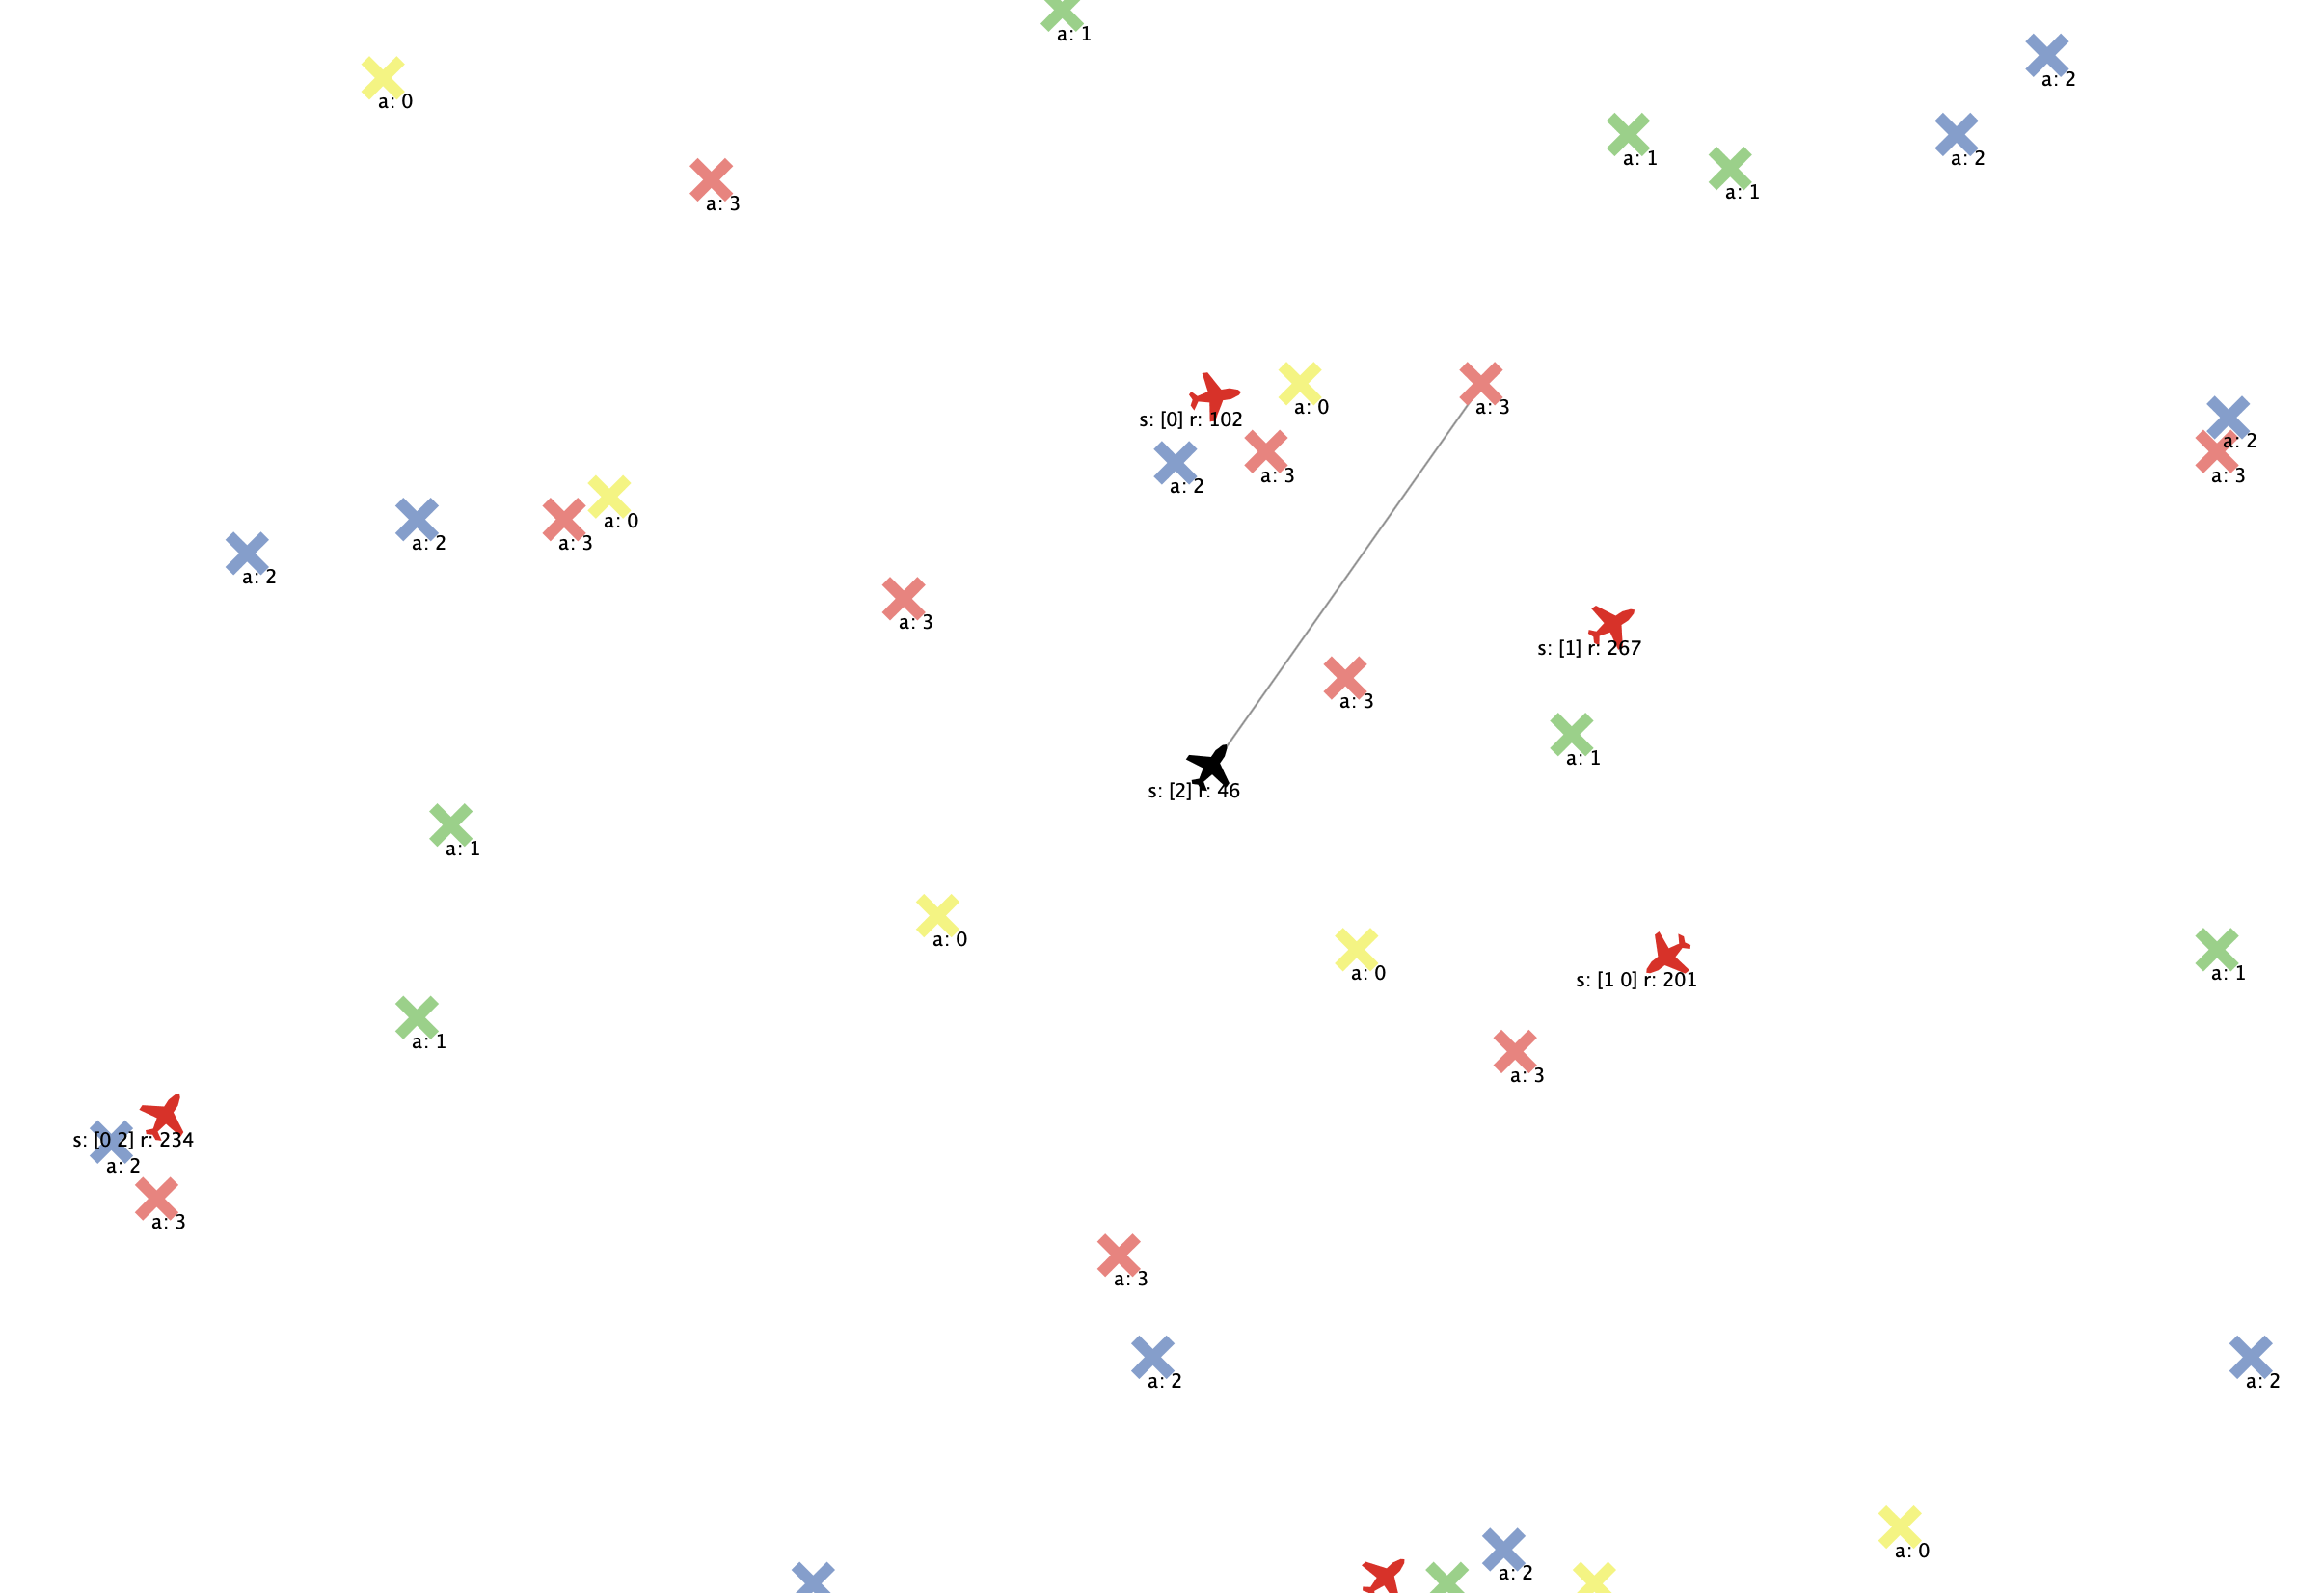
\includegraphics[scale=0.3]{fig/tela01.png}}
		\caption{NetLogo 5.3.1 screen with dropped UAVs in red, in the dynamic scenario}
		\label{fig:screen01}
	\end{center}
\end{figure}

As the quantity of agents changes during the execution, this characteristic gives dynamism to the context. It grants the capacity to analyze the agents' response and to assess the original algorithms in this new dynamic scenario. 

Furthermore, to reduce the standard deviation in the results, all experiments were executed 100 times instead of only 30, as it was done in the original study. It was noticed a decrease in the error using this increased number of runs.

\subsection{Extended Algorithms}\label{sec:changes}
%% Explain the changes made in the original algorithm and their impacts;
%% show a workflow of the main steps of execution;

To address the dynamic scenario described in Section \ref{sec:dynamic_scenario}, changes were implemented in the original algorithms aiming to optimize the tasks allocation. This optimization occurs with the best association of the sensor with the task to be executed, i.e. chose the sensor that has the best quality attribute to that type of task. 

The new procedure is represented by the Algorithm \ref{algo:change} and inserted after the line \label{line:ALini} of the Algorithm \ref{algo:swarm-gap}. Basically, it is done in two main steps: 1) Release all tasks not completed, and 2) Reset the token to reinitialize the task allocation. 

The algorithm implementation uses a communication structure based on a token protocol with a ring architecture (token ring). This solution defines the network behaviour and how the information is exchanged. With this strategy, the first agent visited by the token has more tasks available to choose, and this availability decreases on each visited element in the network.

The first step in the proposed change comes to minimize this limitation. It is represented by the block from Line \ref{line:step1_begin} to \ref{line:step1_end} in the Algorithm \ref{algo:change} and it releases all allocated tasks to guarantee another chance to reallocate the tasks not completed yet.

This procedure aims at optimizing the task reallocation among the remaining UAVs to maximize the best usage of the on-board sensors. Thus, there is a new chance of a UAV be assigned to a task more suitable to its sensors, since the token, running its ring path, is refilled with the released tasks. This provides a chance of another agent being assigned any of these newly available tasks.

%% Comentei as linhas que são comuns aos algoritmos AL, SAL e LAL, deixando apenas o que causa alteração e foi inserido no código original
\begin{algorithm}[!ht]
	\SetAlgoLined
	\DontPrintSemicolon
	\SetKwBlock{Loop}{loop}{end loop}
	\SetKwFor{ForAll}{for all}{do}{end for}
	\SetNlSty{text}{}{:}
	\SetNlSkip{0.3em}	
	
	\caption{Code inserted into the three variants proposed by \textit{Schwarzrock et al.} in \cite{MAS07} to deal better with the dynamism defined by Section \ref{sec:dynamic_scenario} }
	\label{algo:change}
%	Receive Token\; \label{line:receivetoken}
%	Compute available resources $r_i $ \; \label{line:compute_r}
%	\ForAll{ available tasks }{ \label{line:forall}
%		Compute capability $k_{ij}$\; \label{line:compute_k}
%		Compute tendency $T_{\theta_{ij}(st)}$ \;  \label{line:compute_t}
%		\If{ roulette() $< T_{\theta_{ij}(st)}$ and $r_i \geq c_j $}{ %label{line:ini_ifalgo1}
%			Allocate task $j$ to agent $i$ \; \label{line:aloca_sgap}
%			Decrease resource $r_i$ \; \label{line:decrease_r} %label{line:fim_ifalgo1}
%		}
%	}
%	Mark agent as visited in the token\; \label{line:marcavisitado}
%	\vbox{\colorbox{mygray}{\vbox{
	\If{a agent was dropped}{\label{line:step1_begin}
	    \ForAll{agent $j$ alive (not dropped)}{ 
    	    \ForAll{Task $t$ not completed in agent.(TASK\_TO\_DO) list}{ \label{line:notcompleted}
    	        add $t$ to available tasks list in the Token \;
    	        update costs estimated \; \label{line:costs}
    	        adjust stimulus $st_j$ value \; \label{line:stimulus}
            }
        }\label{line:step1_end}
	   
	   \If{$j$ in agent visited list}{\label{line:step2_begin}
	            remove agent from the list visited \;
	            add agent to the not visited list \;
	            clear control parameter of the token \;  \label{line:parameters} %Explain the parameters
	            }
        }\label{line:step2_end}
%    }}}
%	\If{there are still available tasks}{ \label{line:ifstillavatask}
%		Send the token to a not yet visited agent\; \label{line:envia}
%	}
\end{algorithm}

When the tasks are released, it is necessary to update the value of the estimated costs. The tasks not executed should not consume agent resources or leave them locked. This explains the importance of the instruction executed in line \ref{line:costs} of the Algorithm \ref{algo:change}. 

The second step of the proposed proposal, limited by the block of lines \ref{line:step2_begin} to \ref{line:step2_end}, in the Algorithm \ref{algo:change}, is responsible for clearing the history of the visited agents, ensuring the token will pass again through all UAVs that are functionally active. This step gives another chance to all agents to get another task or the same. It is done always maximizing the quality of sensors applied to the tasks. The parameter of line \ref{line:parameters} in the Algorithm \ref{algo:change} refers to the counter of visiting times used by LAL algorithm.

Each algorithm (AL, SAL or LAL) has a quantity of rounds to the token. It is defined to avoid an infinite loop in the token pass and it needs to guarantee a passage through all agents. Regardless of which algorithm is performed, the token reset permits to pass by the UAVs, at least, one more time than what was established. 

It is useful particularly in AL, which uses a greedy strategy to allocate the tasks. This way, it causes a task reallocation among the remaining UAVs. As the token has the opportunity to pass by the agents more often, the number of exchanged messages increases.

Additionally, the $stimulus$ attribute value was updated to adjust the willingness of the agent to perform each task and to analyze its impact on a dynamic context (see line \ref{line:stimulus} in the Algorithm \ref{algo:change}). The initial value used by the original study was $0.6$ as explained in Section \ref{sec:background}, giving a good balance among distance and quality of the sensors at the choose task moment, but different values were tested to measure their impact on the results. The results of these simulations are discussed in Section \ref{sec:discussion}. 

In the original algorithm, all three proposed variants (AL, SAL and LAL) share a common structure formed by some procedures implemented in NetLogo (see Section \ref{sec:background}). The proposed extension was performed in a common part and it is shared by all these variants. Besides what is displayed in Algorithm \ref{algo:change}, auxiliary structures were also created to control the number of dropped and remaining UAVs.

\section{Replications}\label{sec:replications}
Following the overall process defined by action research, and using the new dynamic scenario (Section \ref{sec:dynamic_scenario}), the original algorithms and the extended ones (Section \ref{sec:changes}) were exercised with two replications to identify possible limitations, constraints, and opportunities for improvement. The first replication (Section \ref{sec:original}) was conducted to assess how well the original algorithms work in the dynamic scenario, whereas the second replication (Section \ref{sec:replication}) assesses the extended algorithms in the same dynamic scenario.

All replications in this work use the same time limit of the original study, i.e. a total of 300 ticks. The displacement and task execution have a time consumption and the total time consumed to perform all tasks allocated has to be within this upper limit of 300 ticks.

To perform the replications, some definitions had to be done in terms of parameters applied during the execution of the algorithms. Three independent variables changed during experiments are listed in the following. All the other parameters received the same value used by \textit{Schwarzrock et al.}\cite{MAS07}.
\begin{itemize}
   \item \textit{stimulus}: parameter that defines a priority relation among the distance to the task and the quality of an on board sensors to perform the task. This value is considered during the agent capacity calculation (see Section \ref{sec:background}) and the study by \textit{Ferreira et al.} \cite{ferreira2010robocup} suggested that the best value in most situations of Swarm-GAP strategy application in static scenarios is $0.6$; However, in dynamic scenarios, there is a result impact with different values to \textit{stimulus}. Table \ref{table:stimulus} shows the intervals of difference in results using different values for the \textit{stimulus}. Since the differences are low, value of $0.6$ was fixed as standard to \textit{stimulus} for the final replications so that they have similar conditions to be compare to the results obtained by previous experiments.
   \item \textit{number of executions}: Each replication is repeated $n$ times to generate a set of results and, based on them, calculate the average and standard deviation of each attribute measured during the experiment. The number of executions was increased to 100 runs (instead of 30 used in the original study \cite{MAS07}) for each algorithm aiming at the reduction of the resulting standard deviation, thus getting a higher precision. This increase generated results closer to the normal distribution, minimizing the standard deviation (see a sample result set with 50 executions of the extended SAL algorithm in Figure \ref{fig:fig07}).
   \item \textit{number of UAVs}: Changes in the number of active agents follow what was defined in Section \ref{sec:dynamic_scenario} and force the algorithms to reconfigure the task allocation among the UAVs. This feature makes the scenario dynamic because the number of agent changes during the experiment run time. During the allocation tasks procedure, tasks not finished by the dropped UAVs are reallocated according to the strategy explained in Section \ref{sec:changes}.
\end{itemize}

The focus of the analysis was on the broadest scenario with 9 UAVs. It was chosen because, with smaller scenarios (with lower number of UAVs), the differences in preliminary results were not statistically significant due to high standard deviation. Furthermore, the independent replication was done with the three algorithm variants (AL, SAL and LAL) presented in Section \ref{sec:background}. The source code used during the experiments and the results obtained can be accessed through a link to GitHub repository\footnote{https://github.com/junieramorim/replicationMaterial}.

\begin{table}%[ht]
	\small
	\fontsize{6}{6}\selectfont
	\centering
	\caption{Impacts on the results of the experiments caused by different values of \textit{stimulus} parameter compared with the using of the standard value ($0.6$)}
	\label{table:stimulus}
	
	\begin{tabular}{|c|c|} 
	\hline
		stimulus($st$)
		& results impact\\ [1ex]
	\hline	
	$0.99 \leq st <0.6$           & [1\%,3\%] \\[1ex]
	$0.1 \leq st <0.6$           & [-3\%,-1\%] \\[1ex]
	\hline
	\end{tabular}
\end{table} 



\subsection{First Replication}\label{sec:original}
%%Talk about the replication of the original experiment in a dynamic scenario

The first independent replication to collect empirical results was done with the algorithms proposed in the original work by \textit{Schwarzrock et al.}\cite{MAS07} using the dynamic scenario presented in Section \ref{sec:dynamic_scenario}. It aims to find evidence to either support or refute the conjecture made in the referenced study that it would be fully functional in dynamic scenarios. 

Table \ref{table:table01} shows the results from all algorithms proposed by the original study \cite{MAS07} applied to dynamic context. These results show the total reward obtained with the completed tasks, the total tasks that were finished, the portion of total time ($[0\%,1\%]$) used to perform the maximum possible tasks, the total quality that relates the sensors and the performed tasks, and the number of tokens sent during the execution of the experiments. Some results are normalized to make the comparisons easier. 

\begin{table}%[ht]
	\small
	\fontsize{6}{6}\selectfont
	\centering
	\caption{Total reward, elapsed time, quantity and quality of the completed tasks and number of exchanged messages(tokens sent) for 100 runs of each algorithm with the following attributes: 9 UAVs and 96 tasks in area of 300x240 pixels with deadline of 300 ticks.}
	\label{table:table01}
	
	\begin{tabular}{rrrrr} \hline
		& AL
		& SAL
		& LAL \\ \hline 
		
		& Mean (St.Dev.)  & Mean (St.Dev.)  & Mean (St.Dev.)  \\ [1ex]
		
		\multicolumn{5}{l}{\textbf{Results of the reference study in the same original static context}} \\
	Total reward           & 16.724   ($\pm$2.1908)  & 37.9608  ($\pm$1.1119) & 44.733  ($\pm$1.5961)   \\
	Elapsed time (norm)    & 0.9894   ($\pm$0.0064)  &  0.9763  ($\pm$0.0092) & 0.9693  ($\pm$0.0124)    \\ 
	Comp. tasks (norm)     & 0.2774   ($\pm$0.0276)  &  0.4674  ($\pm$0.0170) & 0.5226  ($\pm$0.0162)    \\ 
	Quality (norm)         & 0.7865   ($\pm$0.0641)  &  0.9680  ($\pm$0.0202) & 0.9752  ($\pm$0.0159)   \\ 
	Sending token          &  9.8667  ($\pm$1.1958)  &  9.7000  ($\pm$1.2360) & 51.500 ($\pm$1.4797)   \\ [1ex]
		
		\multicolumn{5}{l}{\textbf{Independent replication using the dynamic context (number of UAVs changes)}} \\
	Total reward           & 8.6995  ($\pm$1.9489)  & 23.6496 ($\pm$2.6004) &  28.348  ($\pm$2.8464)  \\
	Elapsed time (norm)    & 0.9767  ($\pm$0.0135)  & 0.9652  ($\pm$0.0220) &  0.9513  ($\pm$0.0281)  \\ 
	Comp. tasks (norm)     & 0.1418  ($\pm$0.0281)  & 0.2852  ($\pm$0.0315) &  0.3278  ($\pm$0.0328)  \\ 
	Quality (norm)         & 0.5753  ($\pm$0.1421)  & 0.5751  ($\pm$0.1358) &  0.5858  ($\pm$0.1424)  \\ 
	Sending token          & 10.0900 ($\pm$1.3416)  & 9.9800  ($\pm$1.1805) &  49.4600 ($\pm$1.9562)  \\ [1ex]

		\hline
	\end{tabular}
\end{table} 






The analysis concentrates in all results of the experiments that used more agents (9 UAVs) and tasks (96) since they represent the highest value difference between the dependent variables of the original study and those obtained in the dynamic scenario. All other results are available in the repository\footnote{https://github.com/junieramorim/replicationMaterial}. Overall, these results suggest that the original algorithms work in a dynamic scenario due to the average level obtained with no inconsistent value to all variables, e.g., zero or negative values. Nevertheless, those results were significantly different from the values obtained by the original work.

Graphs comparing the results obtained with this first replication in the dynamic scenario (Section \ref{sec:dynamic_scenario}) and the reproduction of original study in the static context are presented in the following, along with a related discussion.

The metric concerning the number of finished tasks (Figure \ref{fig:fig04}) presented a reduction greater than $40\%$ due to the fact that there are fewer agents performing the mission. Indeed, as the dynamic scenario makes the number of agents decreases at runtime, not all tasks allocated are completed, which explains this difference. 

Another metric that suffered a significant degradation (greater than $30\%$) was the quality, as seen in Figure \ref{fig:fig03}. This quality is calculated as a sum of the sensors compatibility with the tasks, i.e., each sensor has a number between 0 and 1 that defines how suitable this sensor is to be used in a specific task, correlating the sensors characteristics and the type of task. This number ($Q_{ij}$) defines the agent $i$ quality to perform the task $j$ and it is used to calculate the agent capability ($k_{ij}$) (Equation \ref{eq:capability}).

The reduction in this attribute was in consequence of the algorithms characteristics that simply discard the allocated tasks, from the available tasks list, when the agent is shut down. These tasks are not reallocated among the remaining UAVs, thus reducing the quality of the sensors related to the finished tasks.

\begin{figure}[h!]
	\begin{center}
		%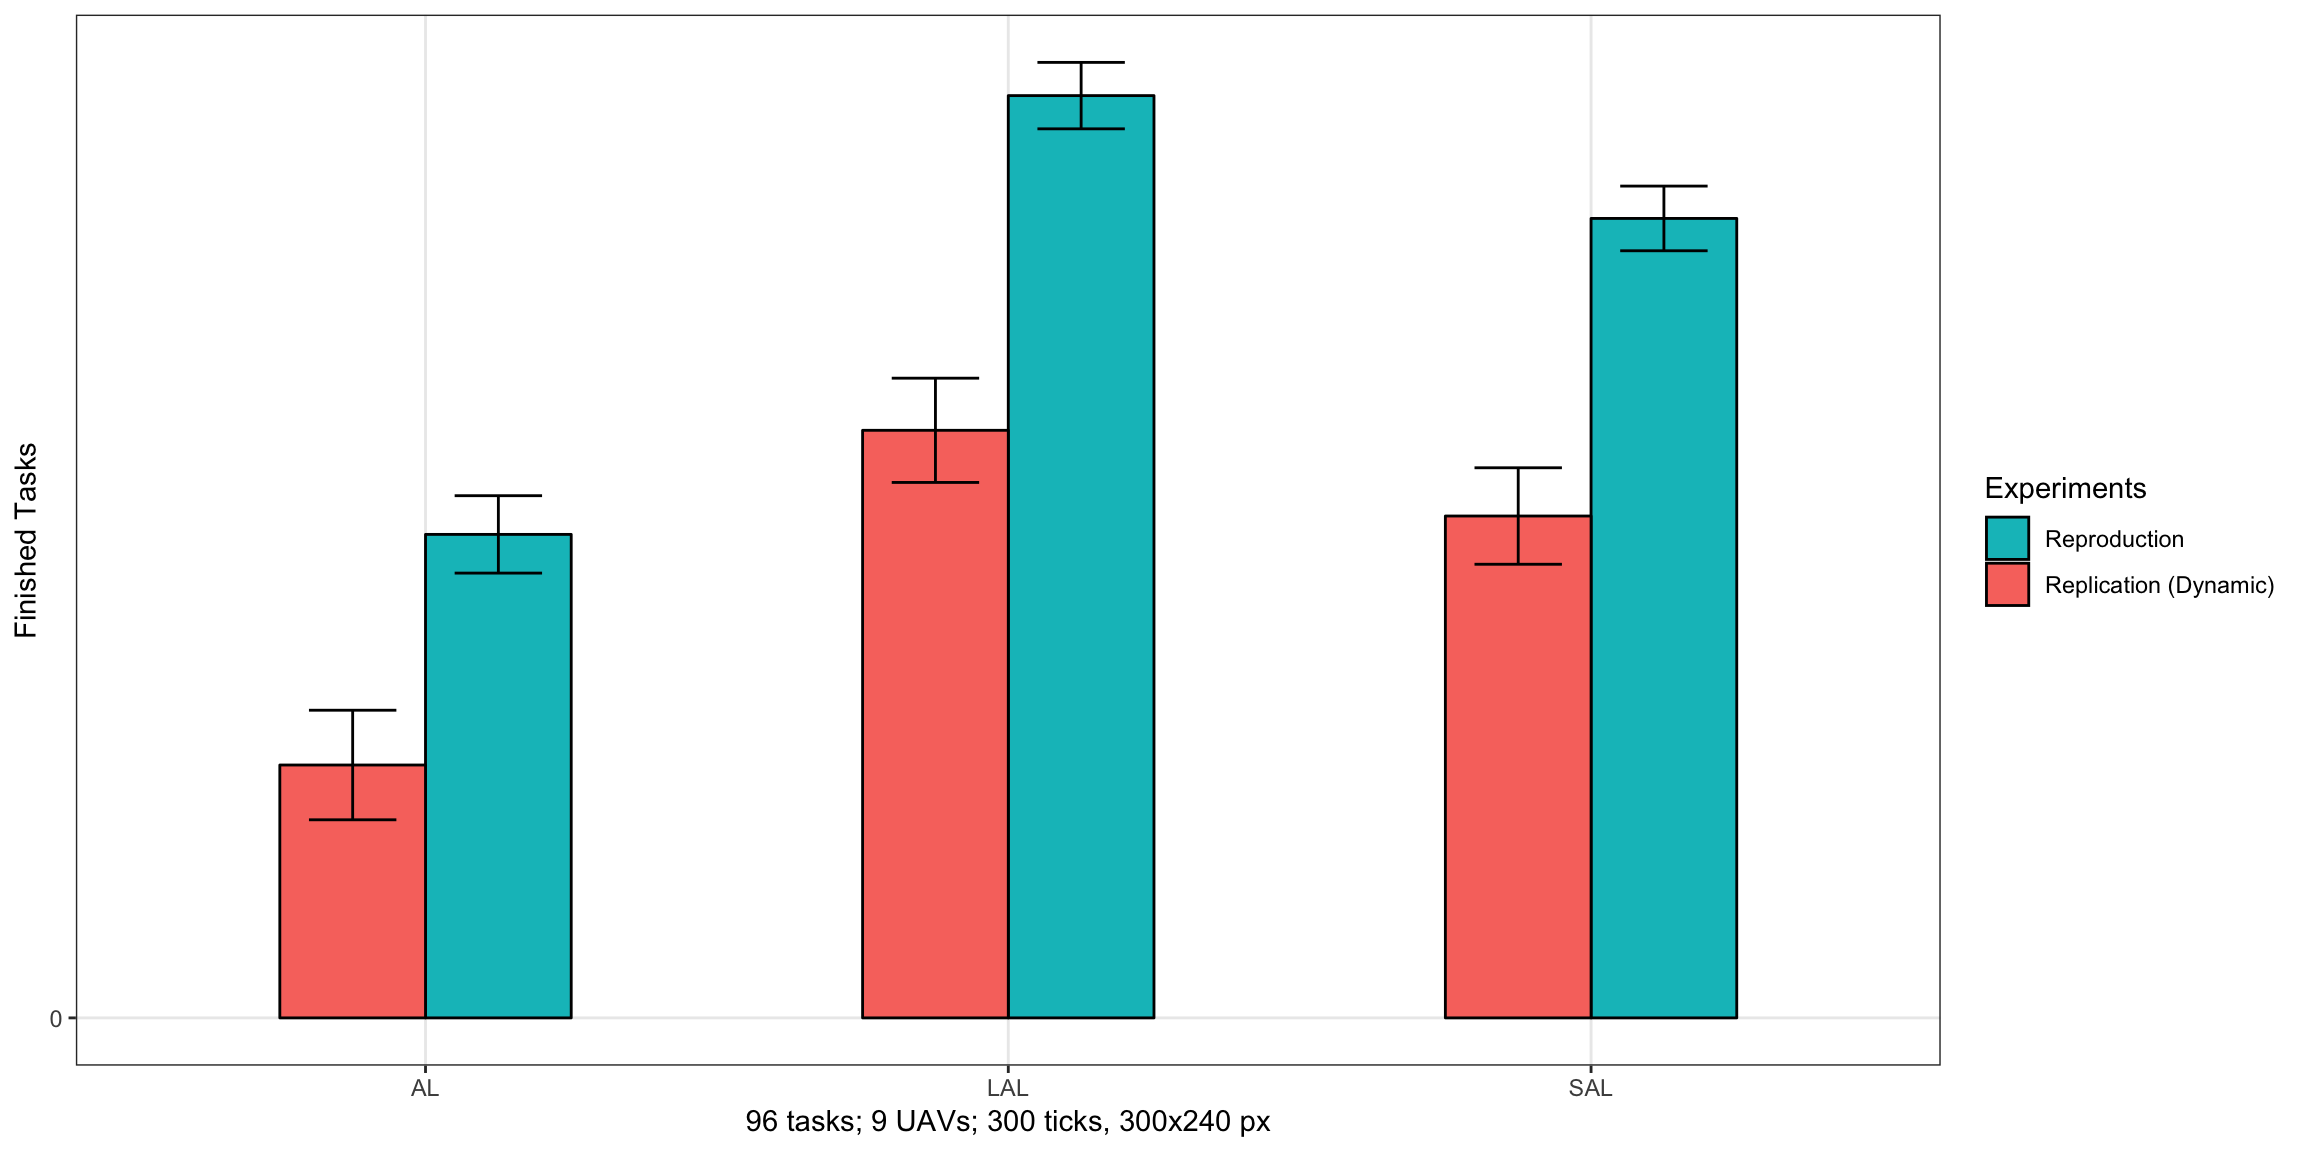
\includegraphics[scale=0.15]{fig/finished_orig.png}
		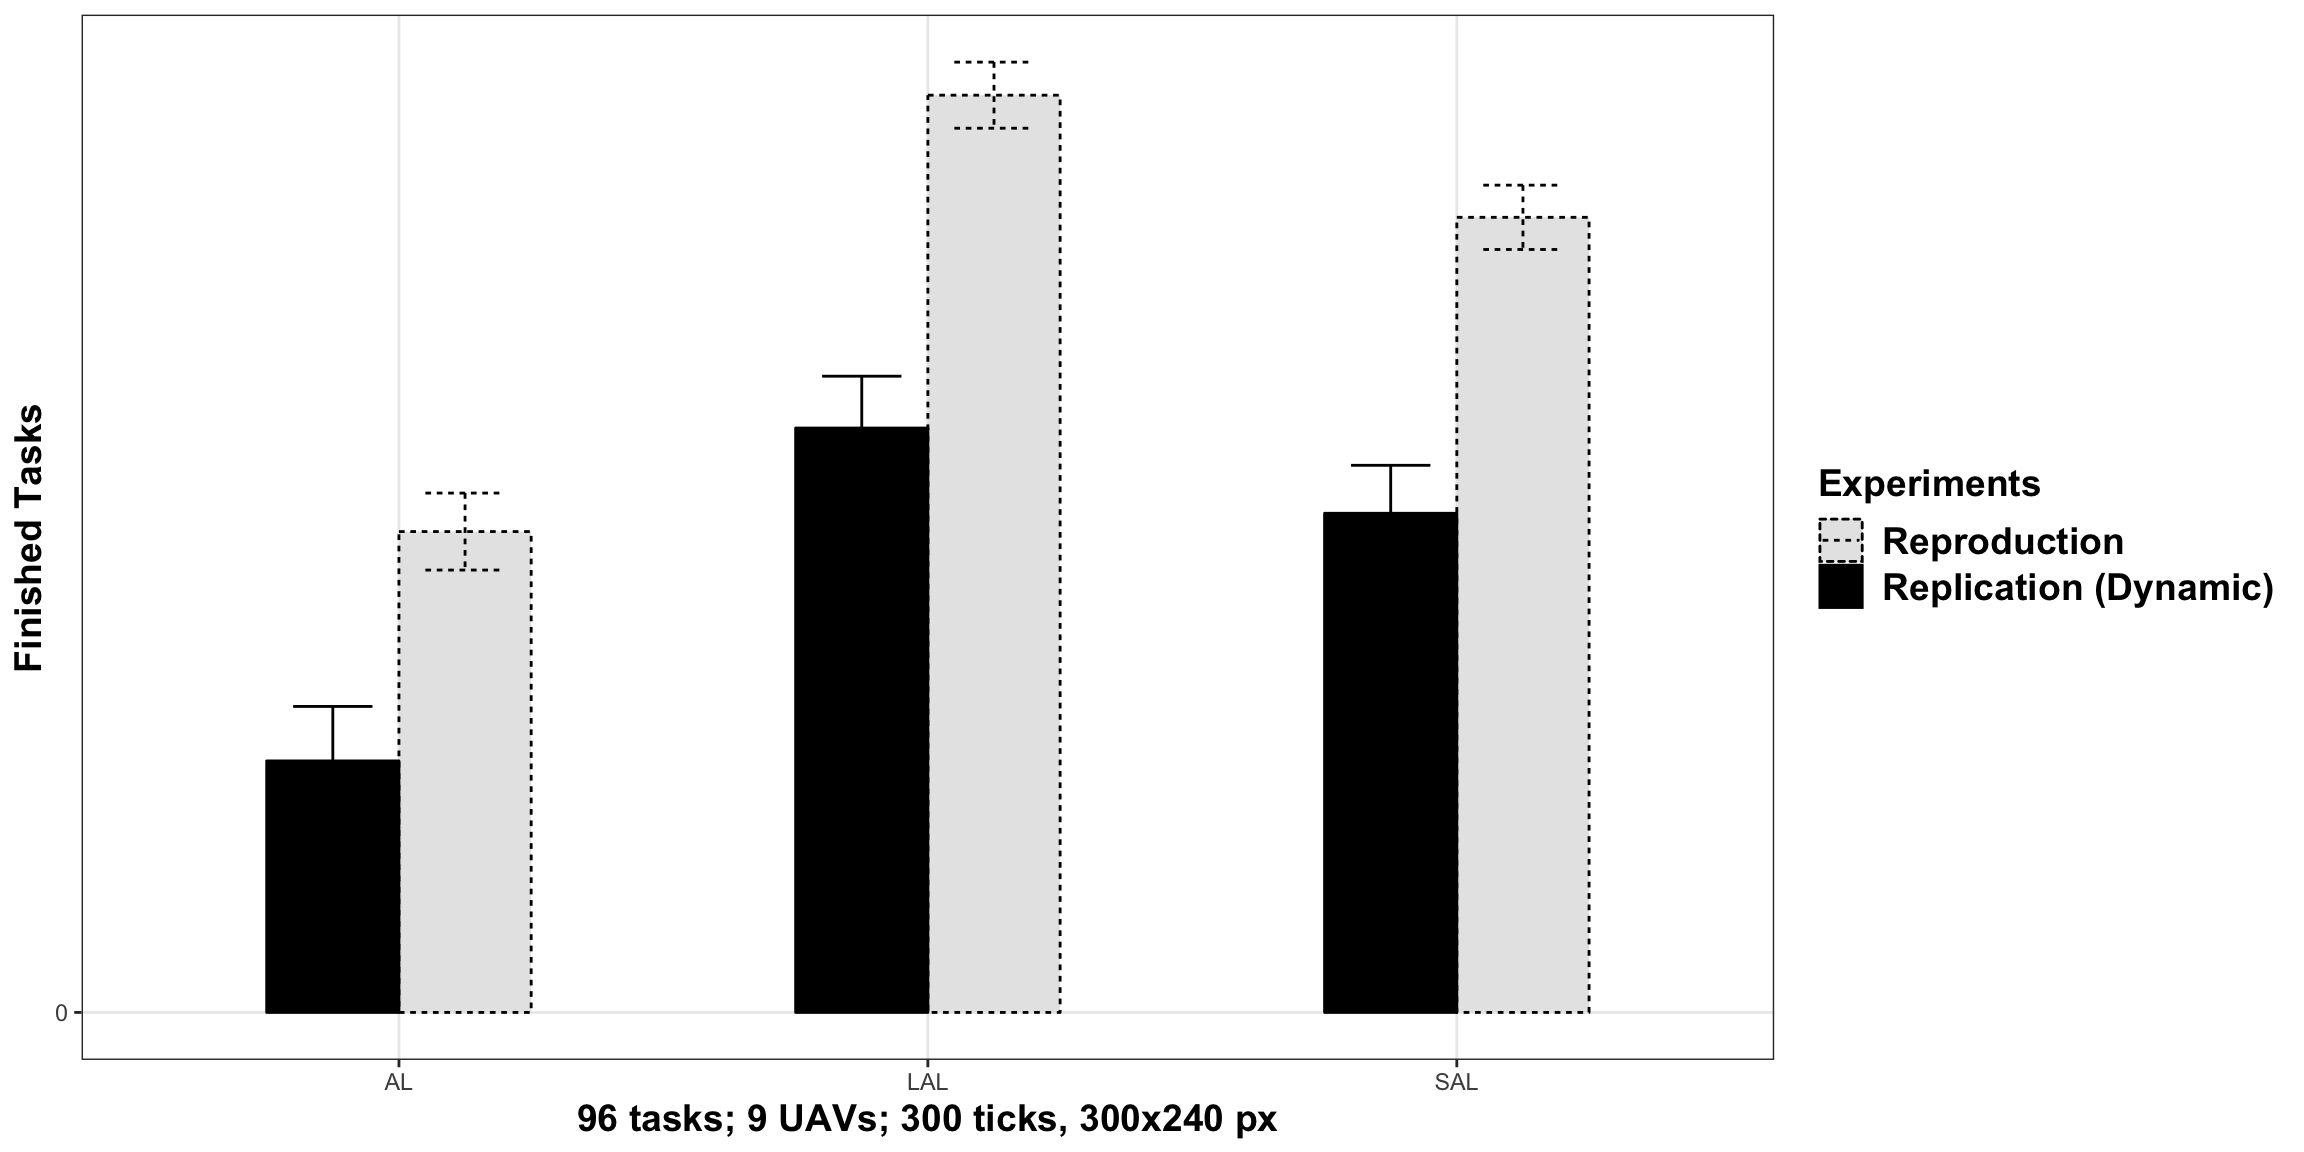
\includegraphics[scale=0.15]{fig/GRAPH01.png}
		\caption{Finished Tasks (96 tasks; 9 UAVs; 300 x 240; 300 ticks)}
		\label{fig:fig04}
	\end{center}
\end{figure}

\begin{figure}[h!]
	\begin{center}
		%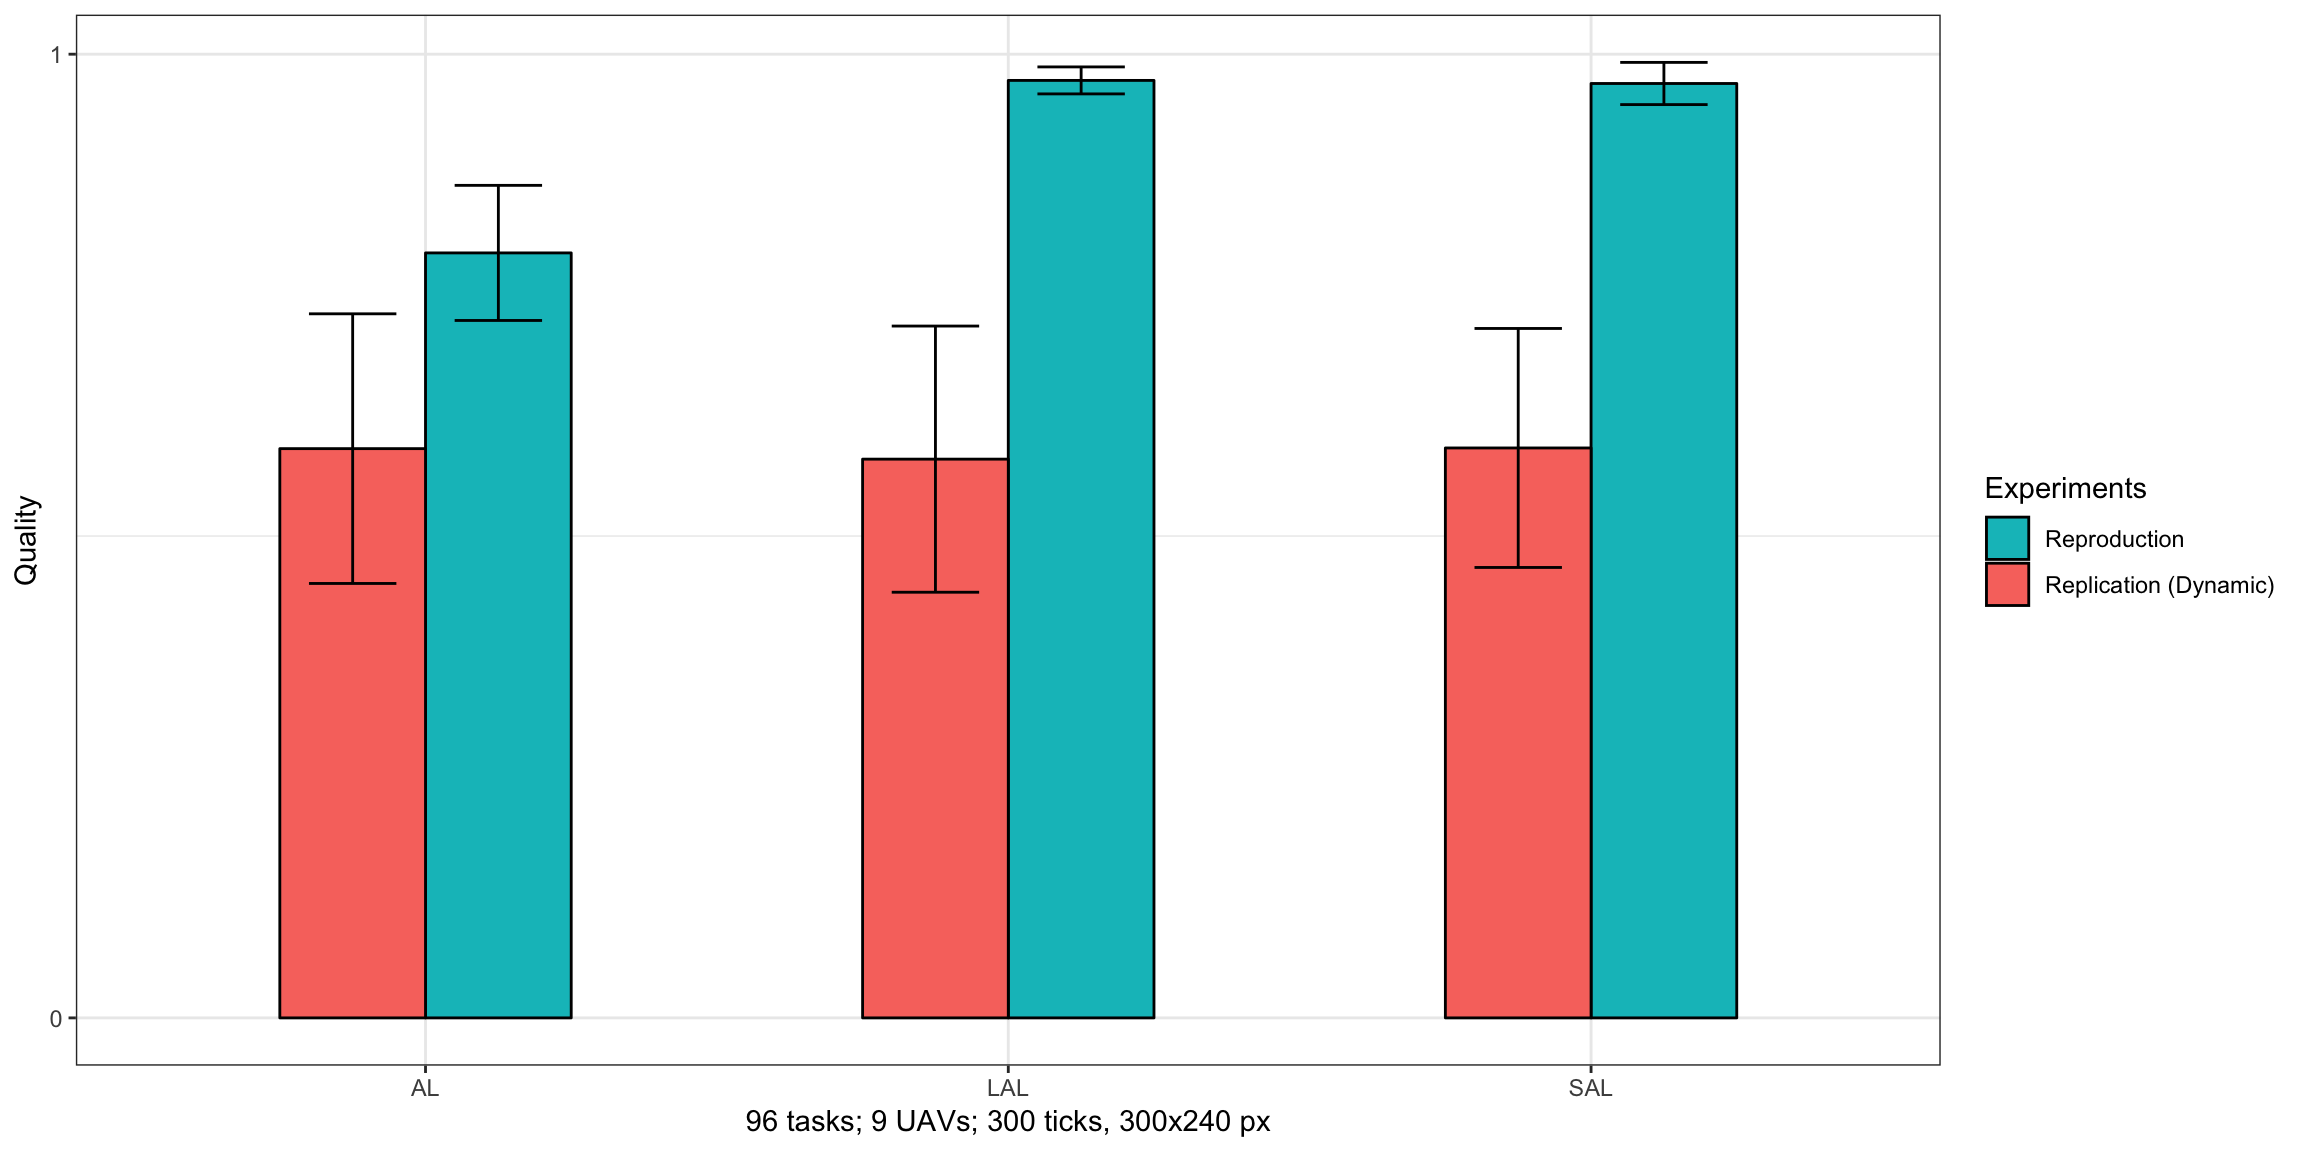
\includegraphics[scale=0.15]{fig/quality_orig.png}
		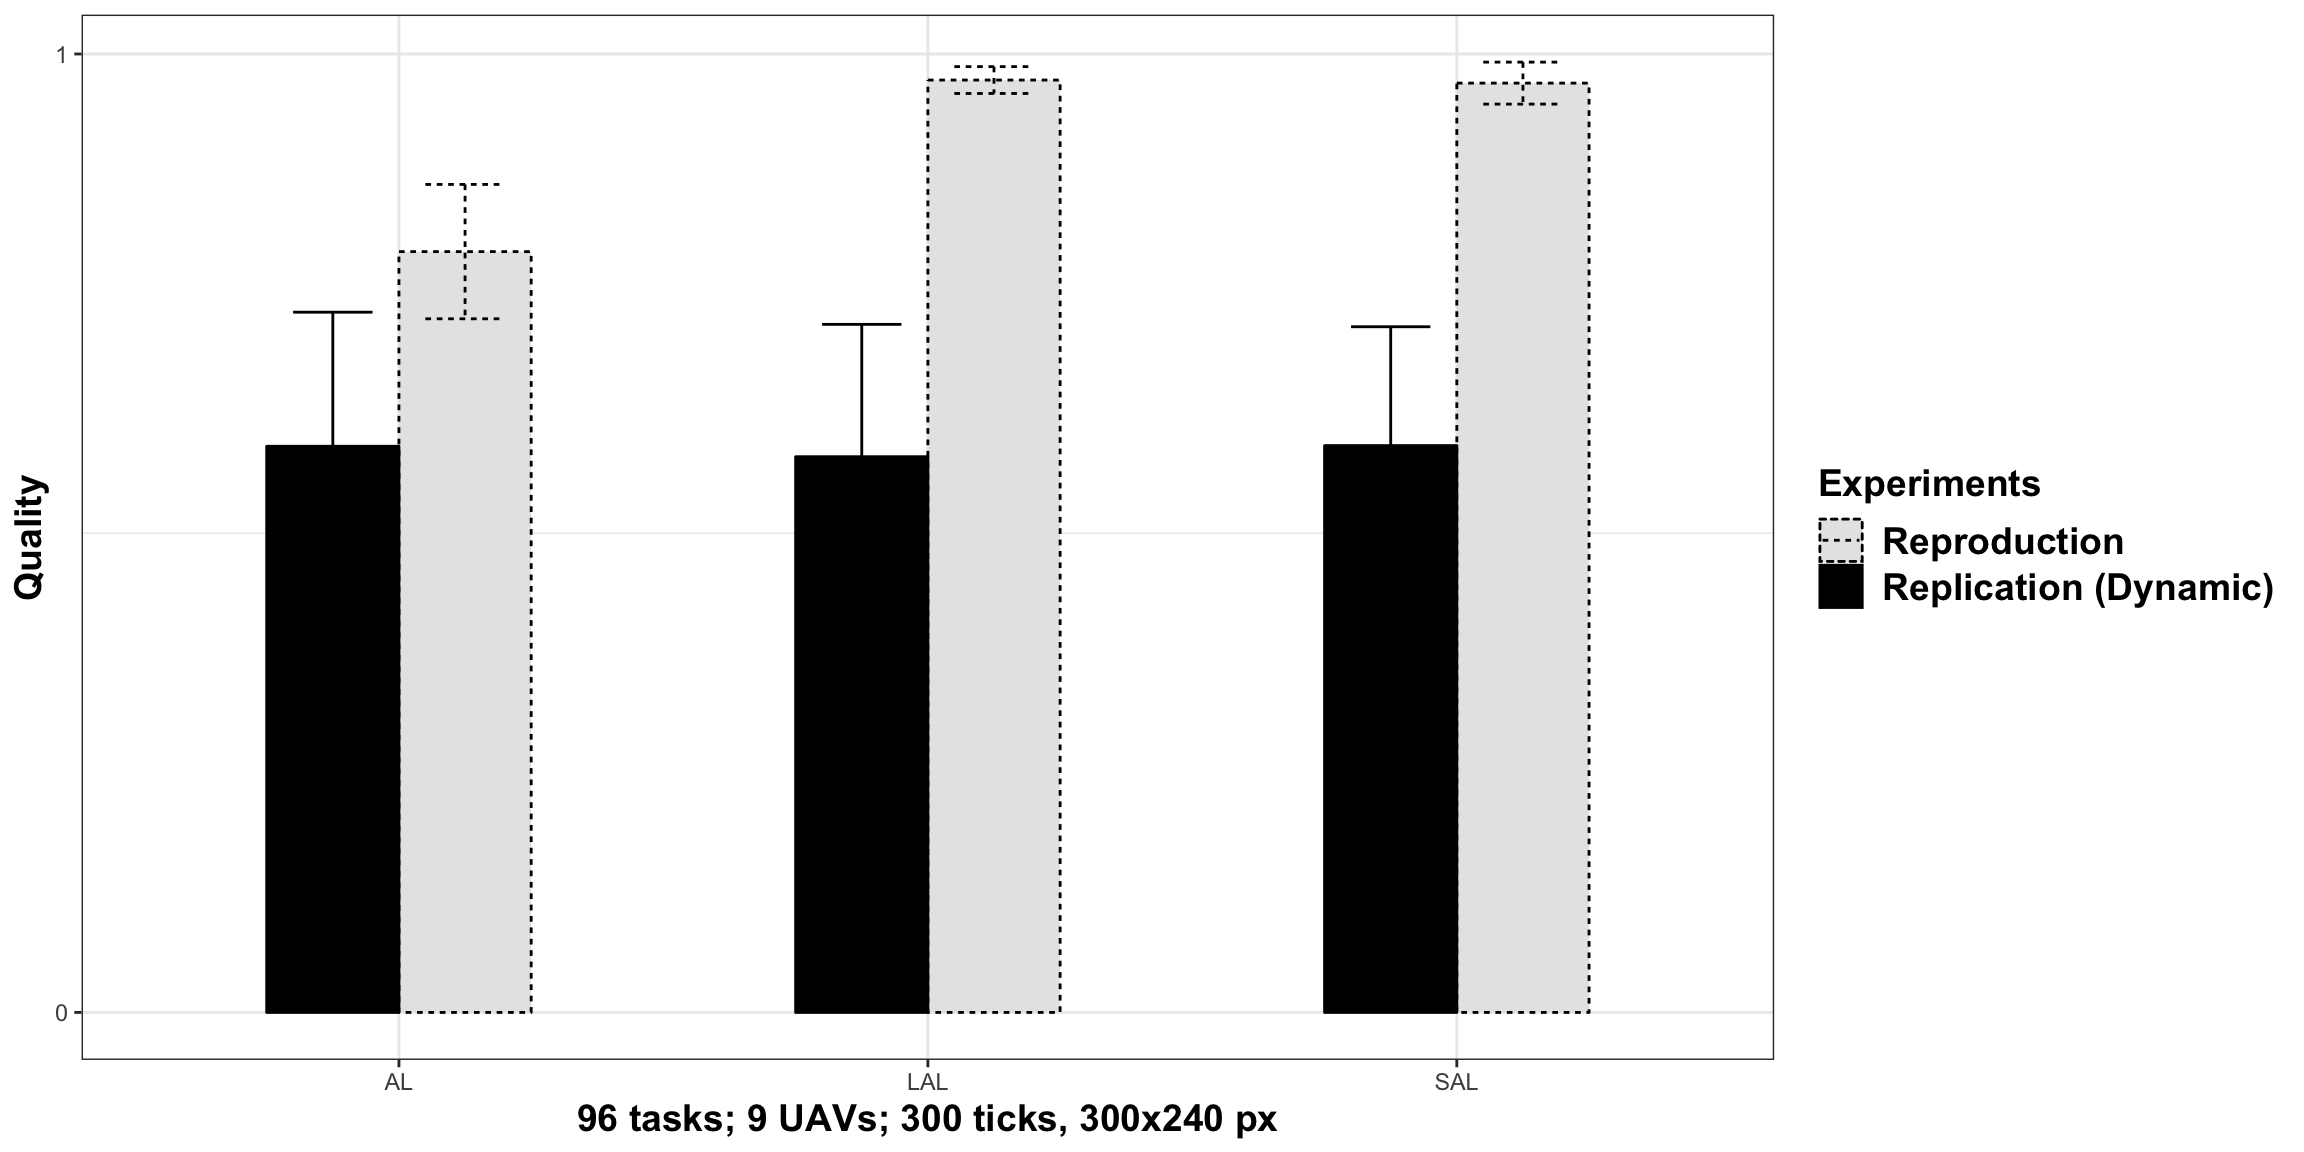
\includegraphics[scale=0.15]{fig/GRAPH02.png}
		\caption{Quality (96 tasks; 9 UAVs; 300 x 240; 300 ticks)}
		\label{fig:fig03}
	\end{center}
\end{figure}

On another hand, other metrics presented very similar results to the original experiment, as the number of messages exchanged, and the total reward and execution time.

The ring network relies on passing a token to each element. Even reducing the number of elements, the number of messages did not decrease because the token runs while it has tasks available or there is a UAV not visited by the token.

As the total reward is the sum of the UAV capability $k_{ij}$ related to the finished tasks, and the capability, defined in \cite{MAS07}, is a function of distance to the task and sensor quality, the reduction of quality causes a proportional decrease in the capability, as confirmed by Figure \ref{fig:fig02}.

\begin{figure}[h!]
	\begin{center}
		%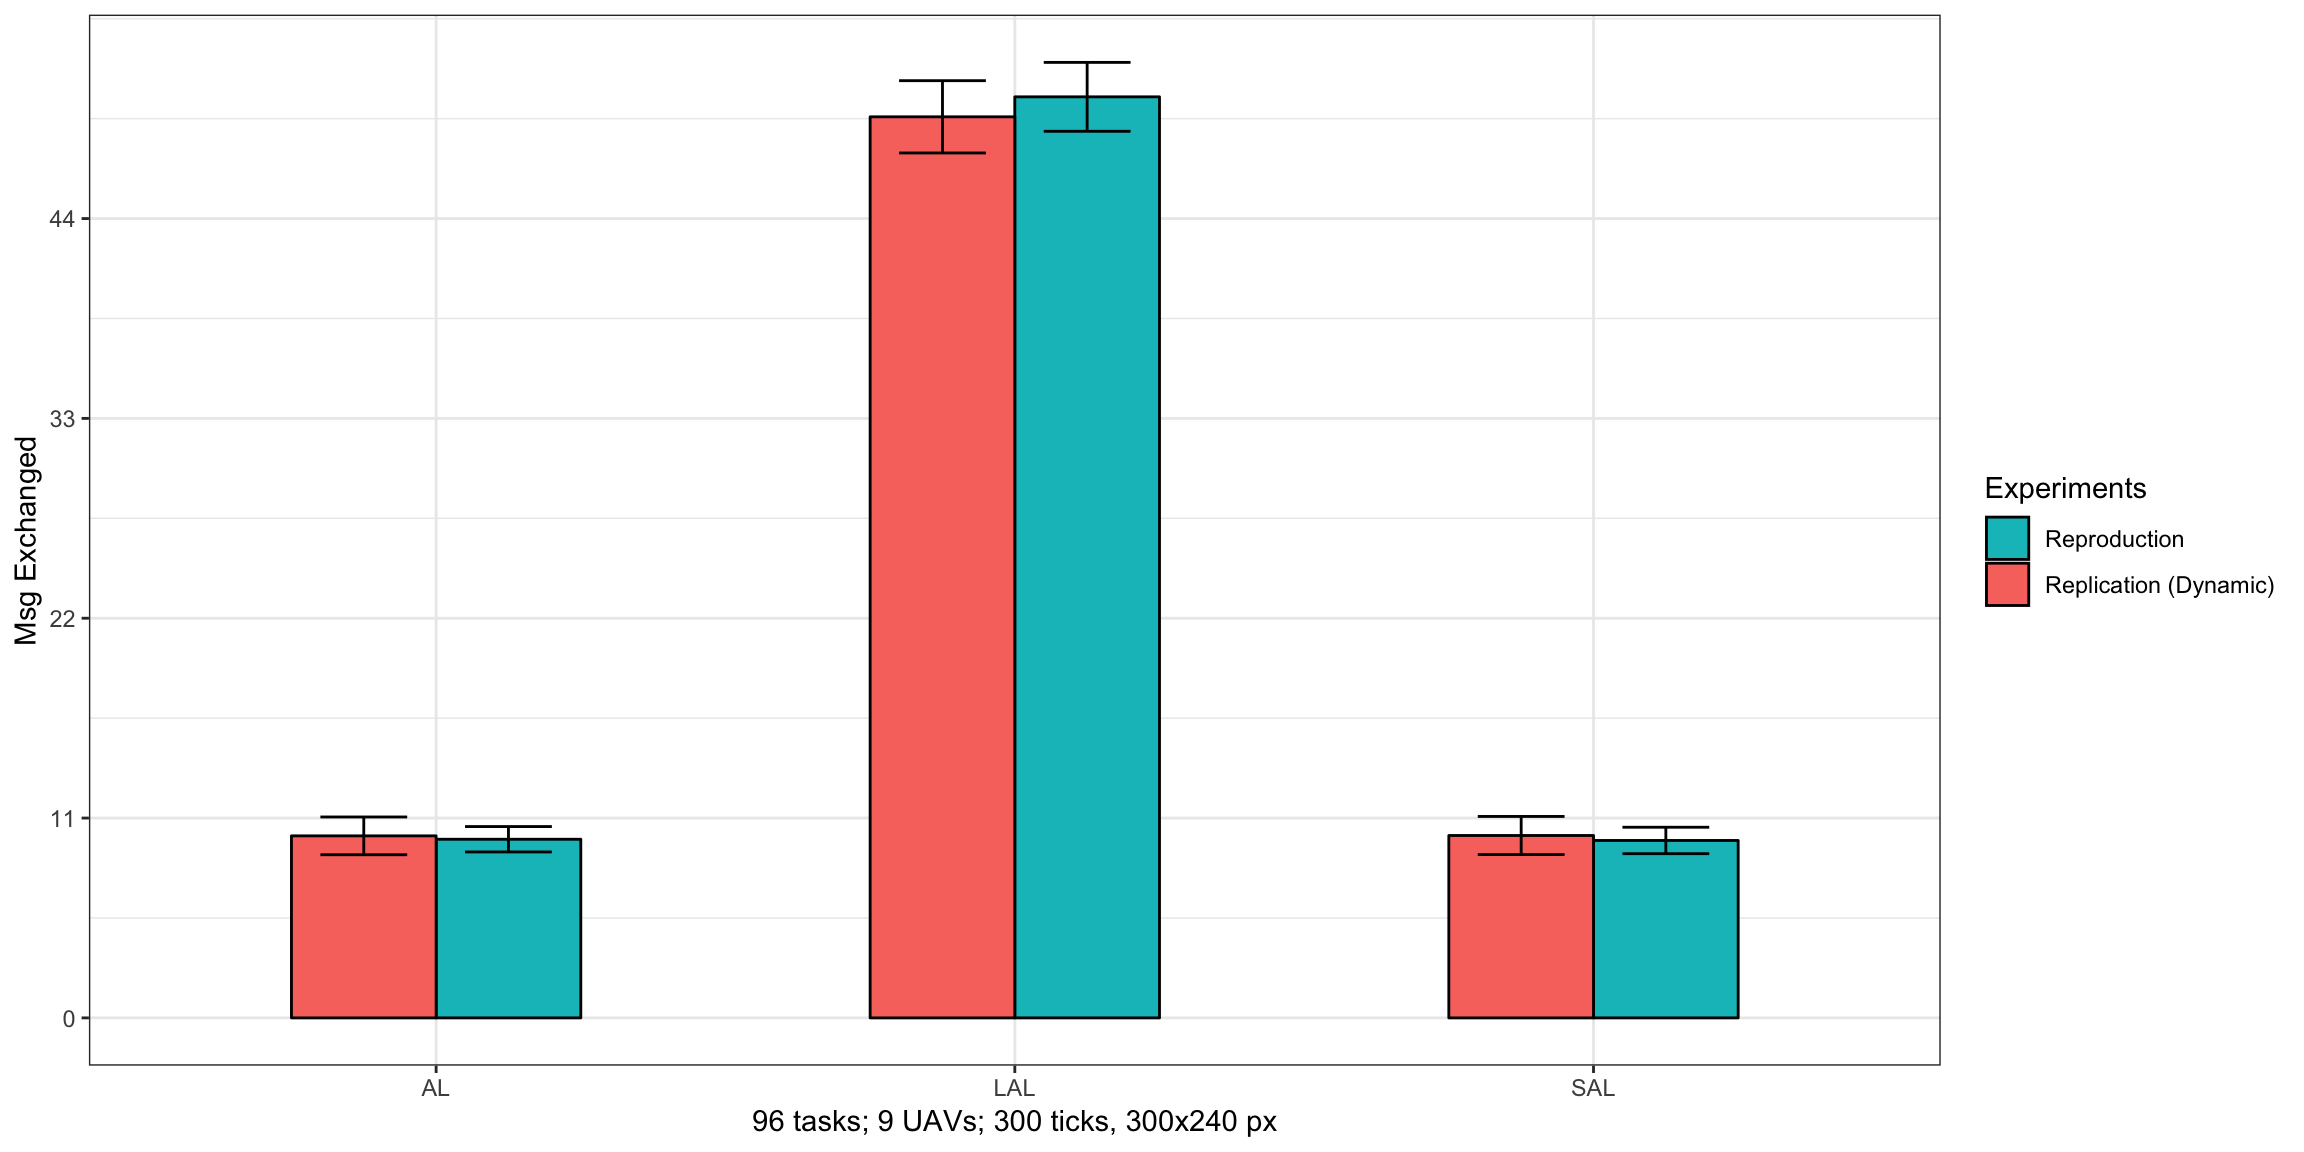
\includegraphics[scale=0.15]{fig/msg_orig.png}
		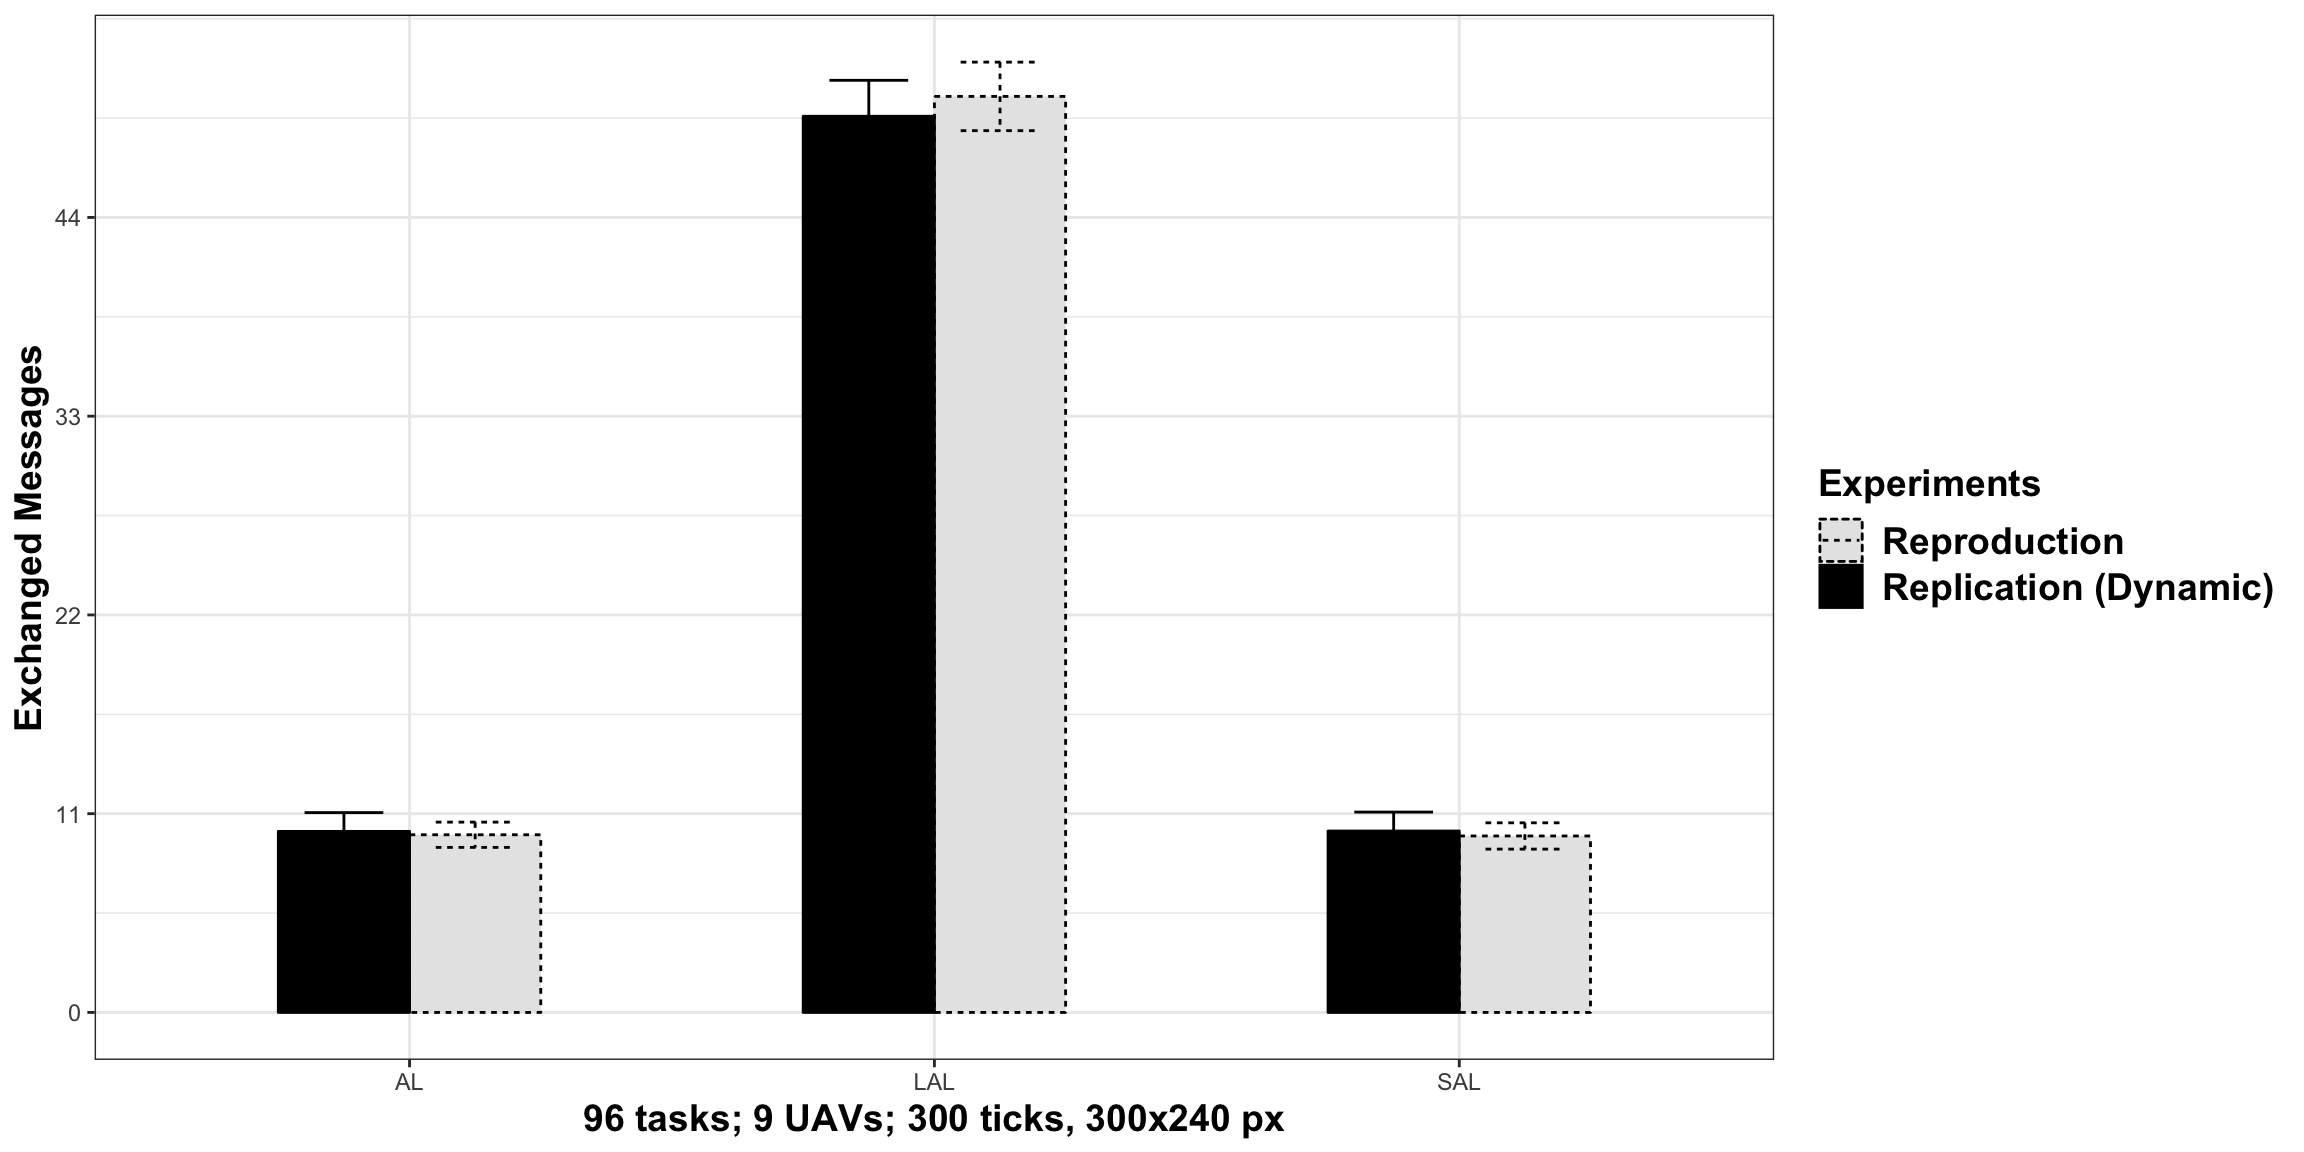
\includegraphics[scale=0.15]{fig/GRAPH03.png}
		\caption{Exchanged Messages  (96 tasks; 9 UAVs; 300 x 240; 300 ticks)}
		\label{fig:fig01}
	\end{center}
\end{figure}

\begin{figure}[h!]
	\begin{center}
		%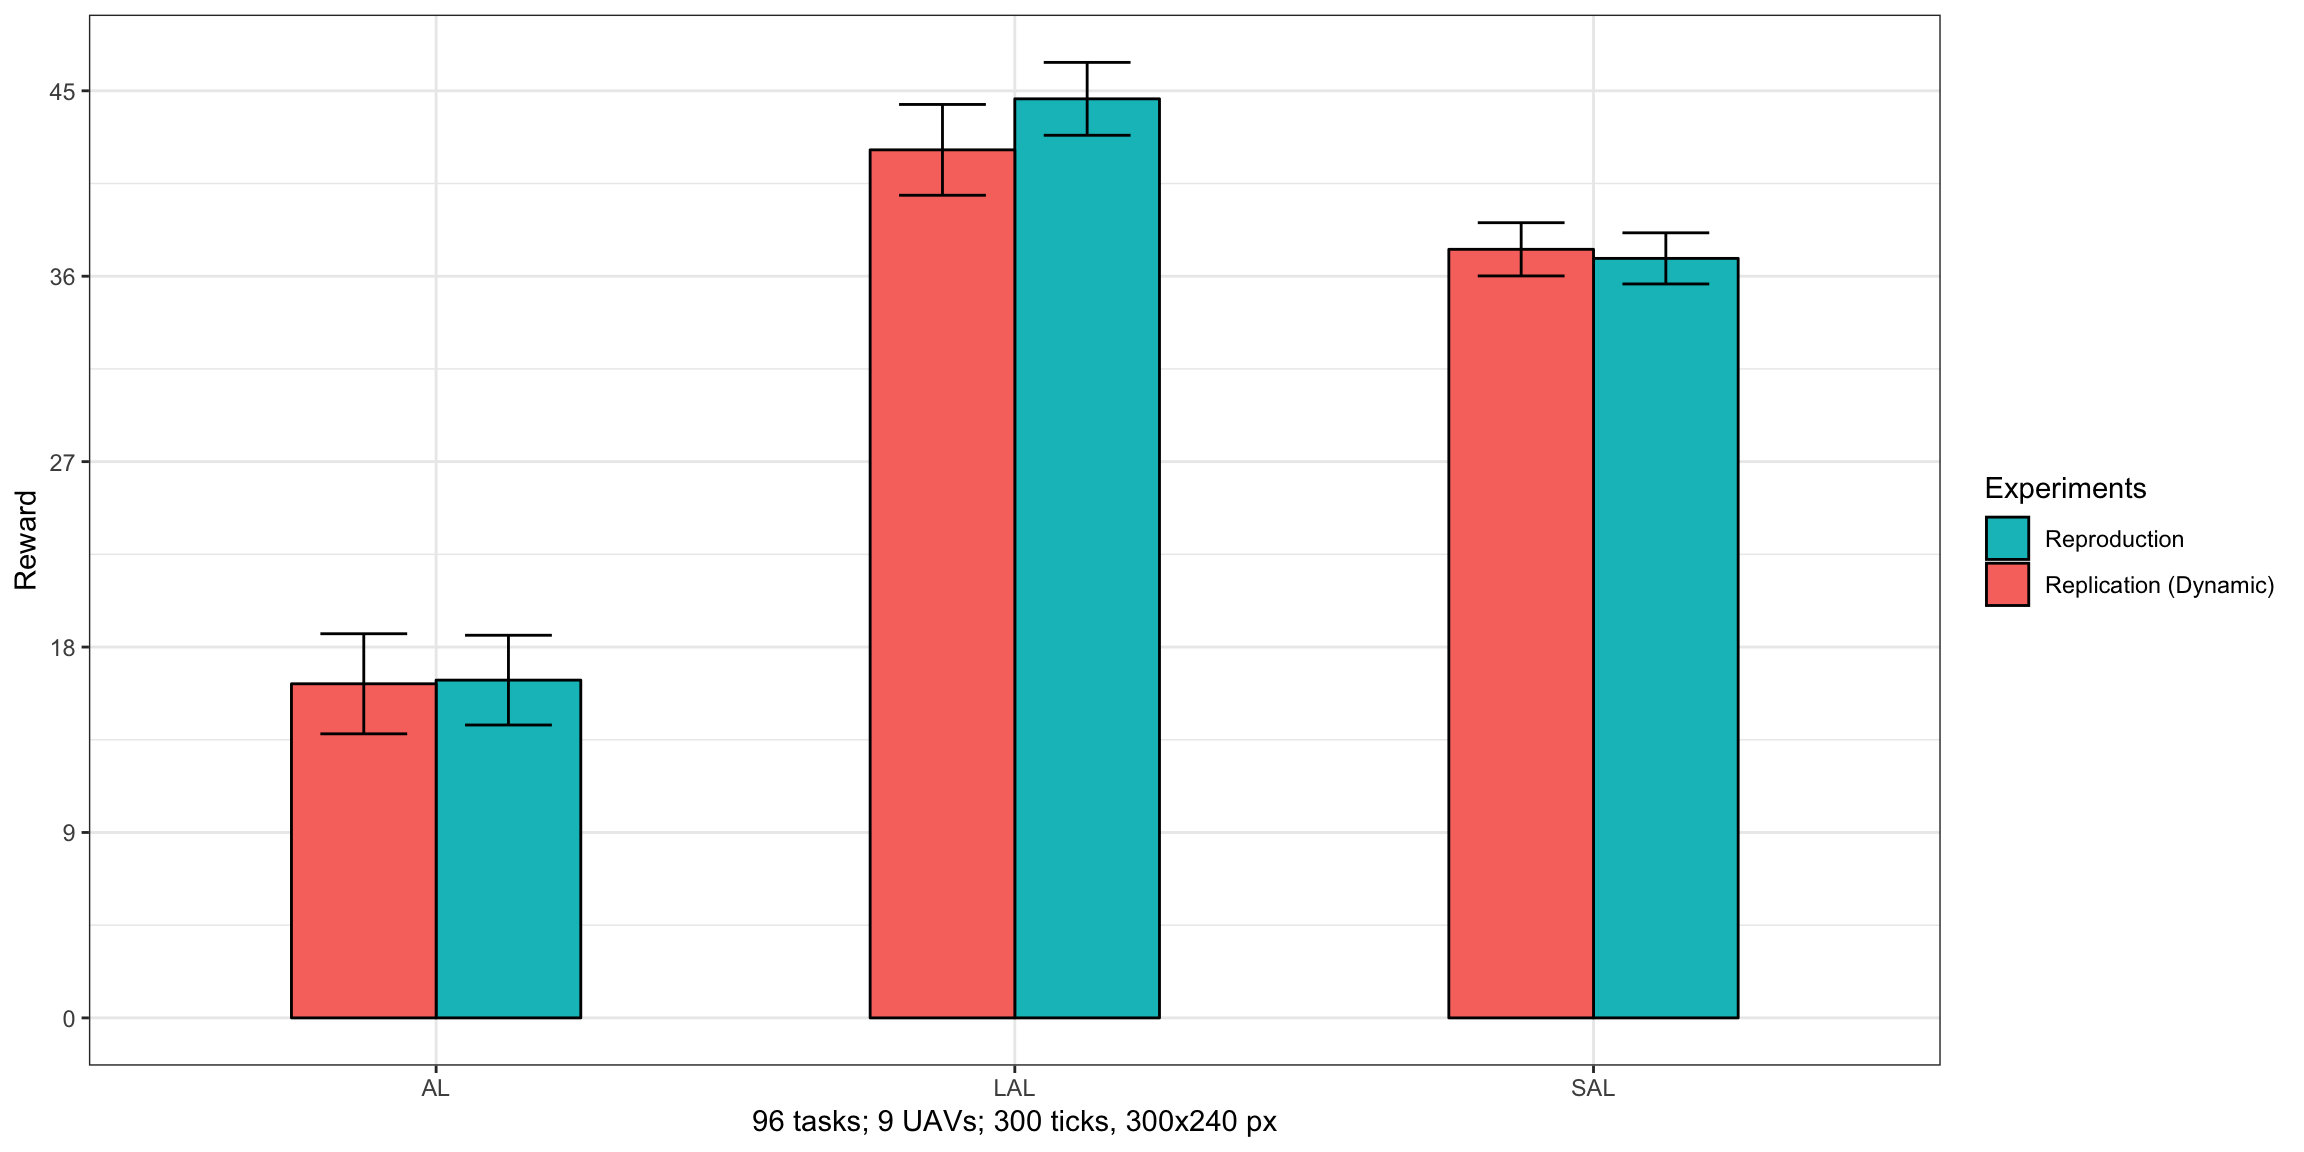
\includegraphics[scale=0.15]{fig/reward_orig.png}
		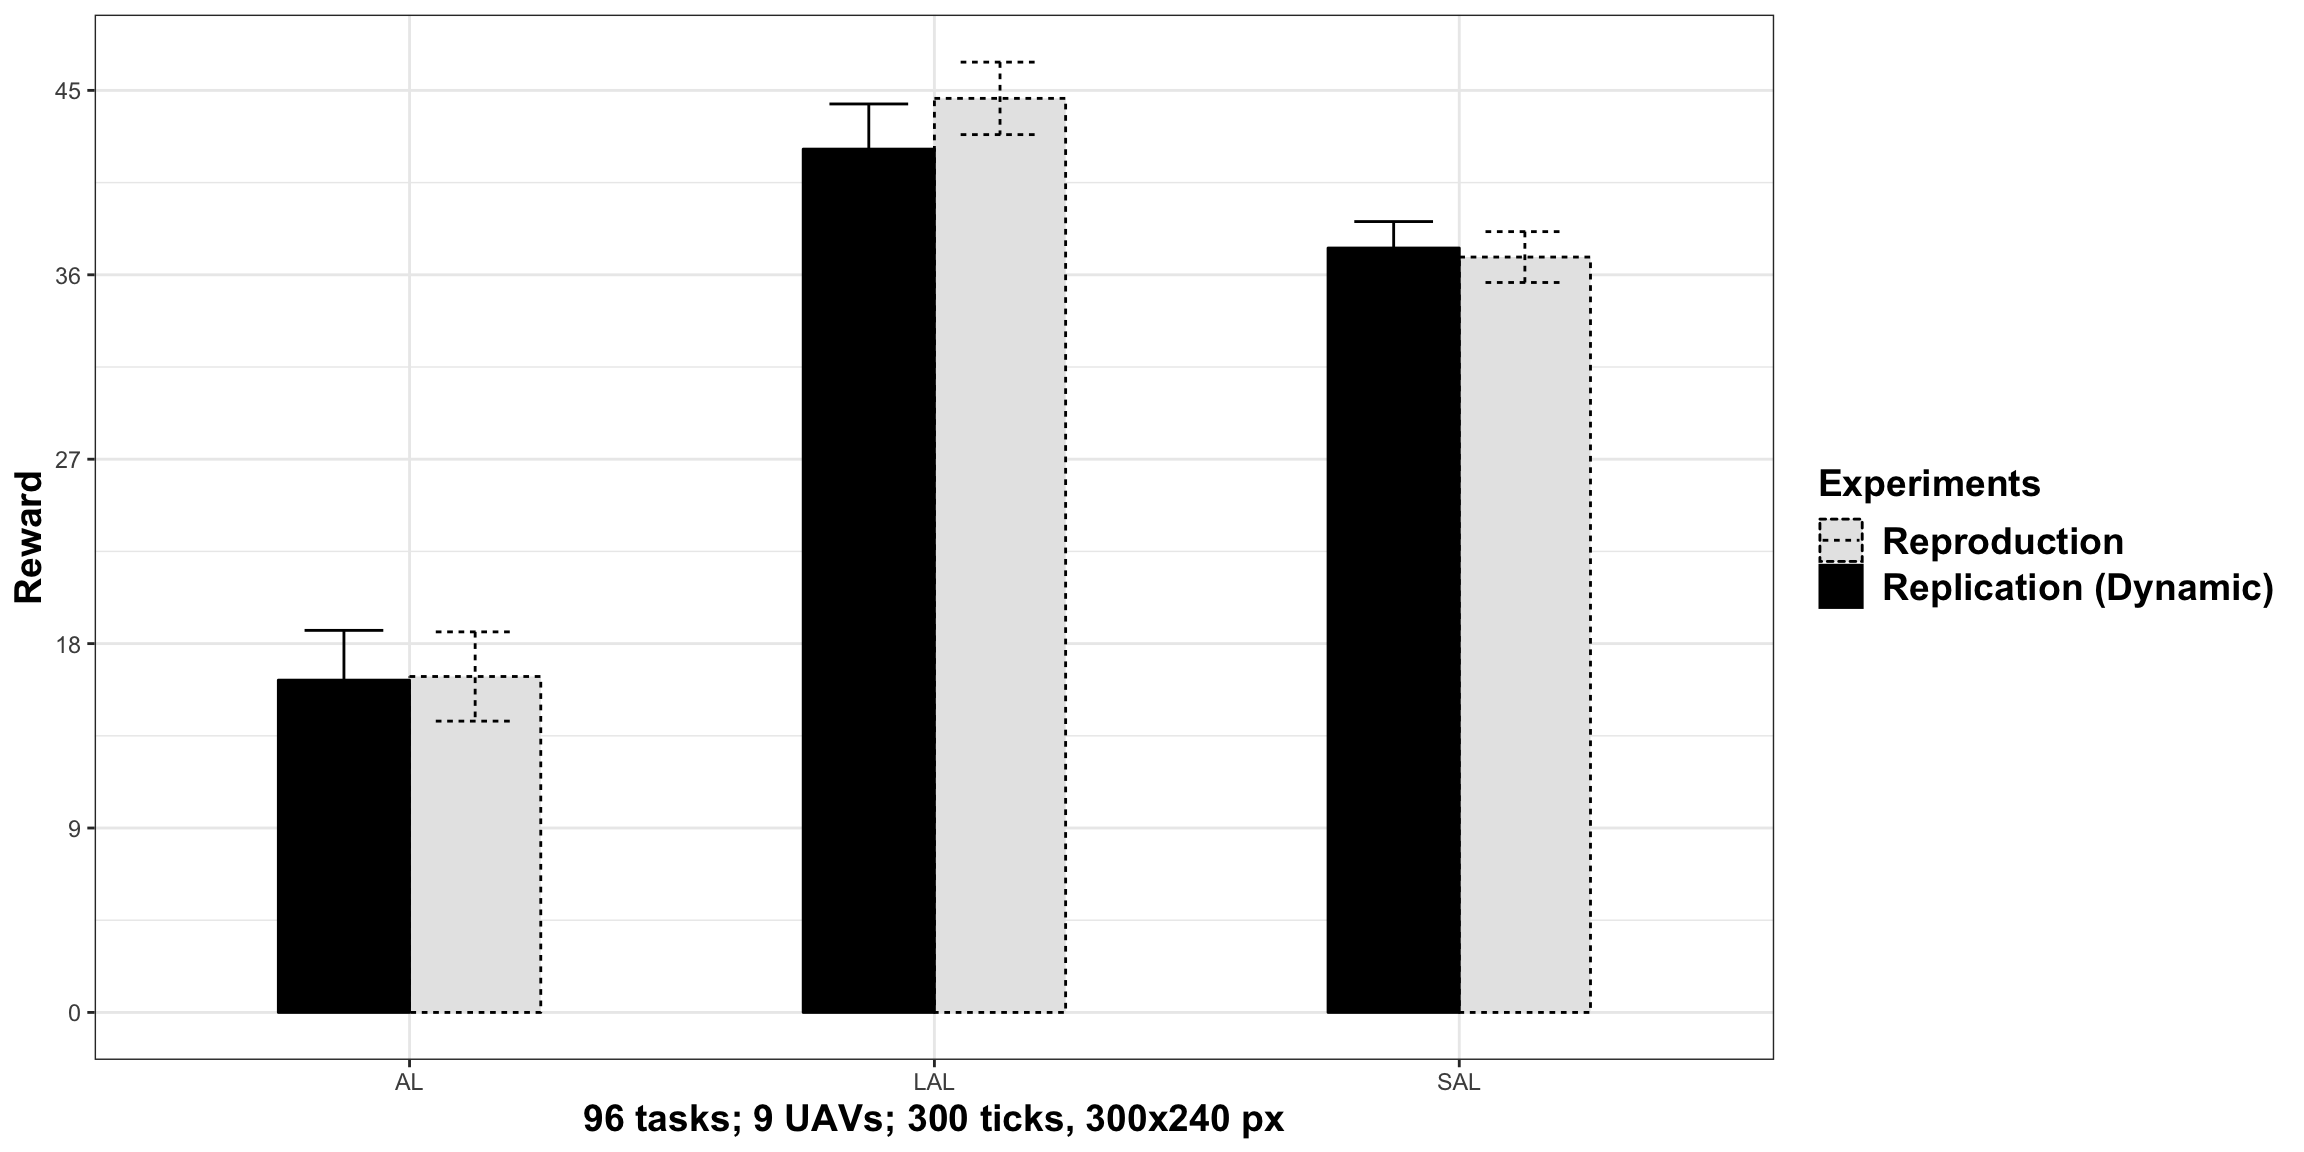
\includegraphics[scale=0.15]{fig/GRAPH04.png}
		\caption{Total Reward (96 tasks; 9 UAVs; 300 x 240; 300 ticks)}
		\label{fig:fig02}
	\end{center}
\end{figure}

\begin{figure}[h!]
	\begin{center}
		%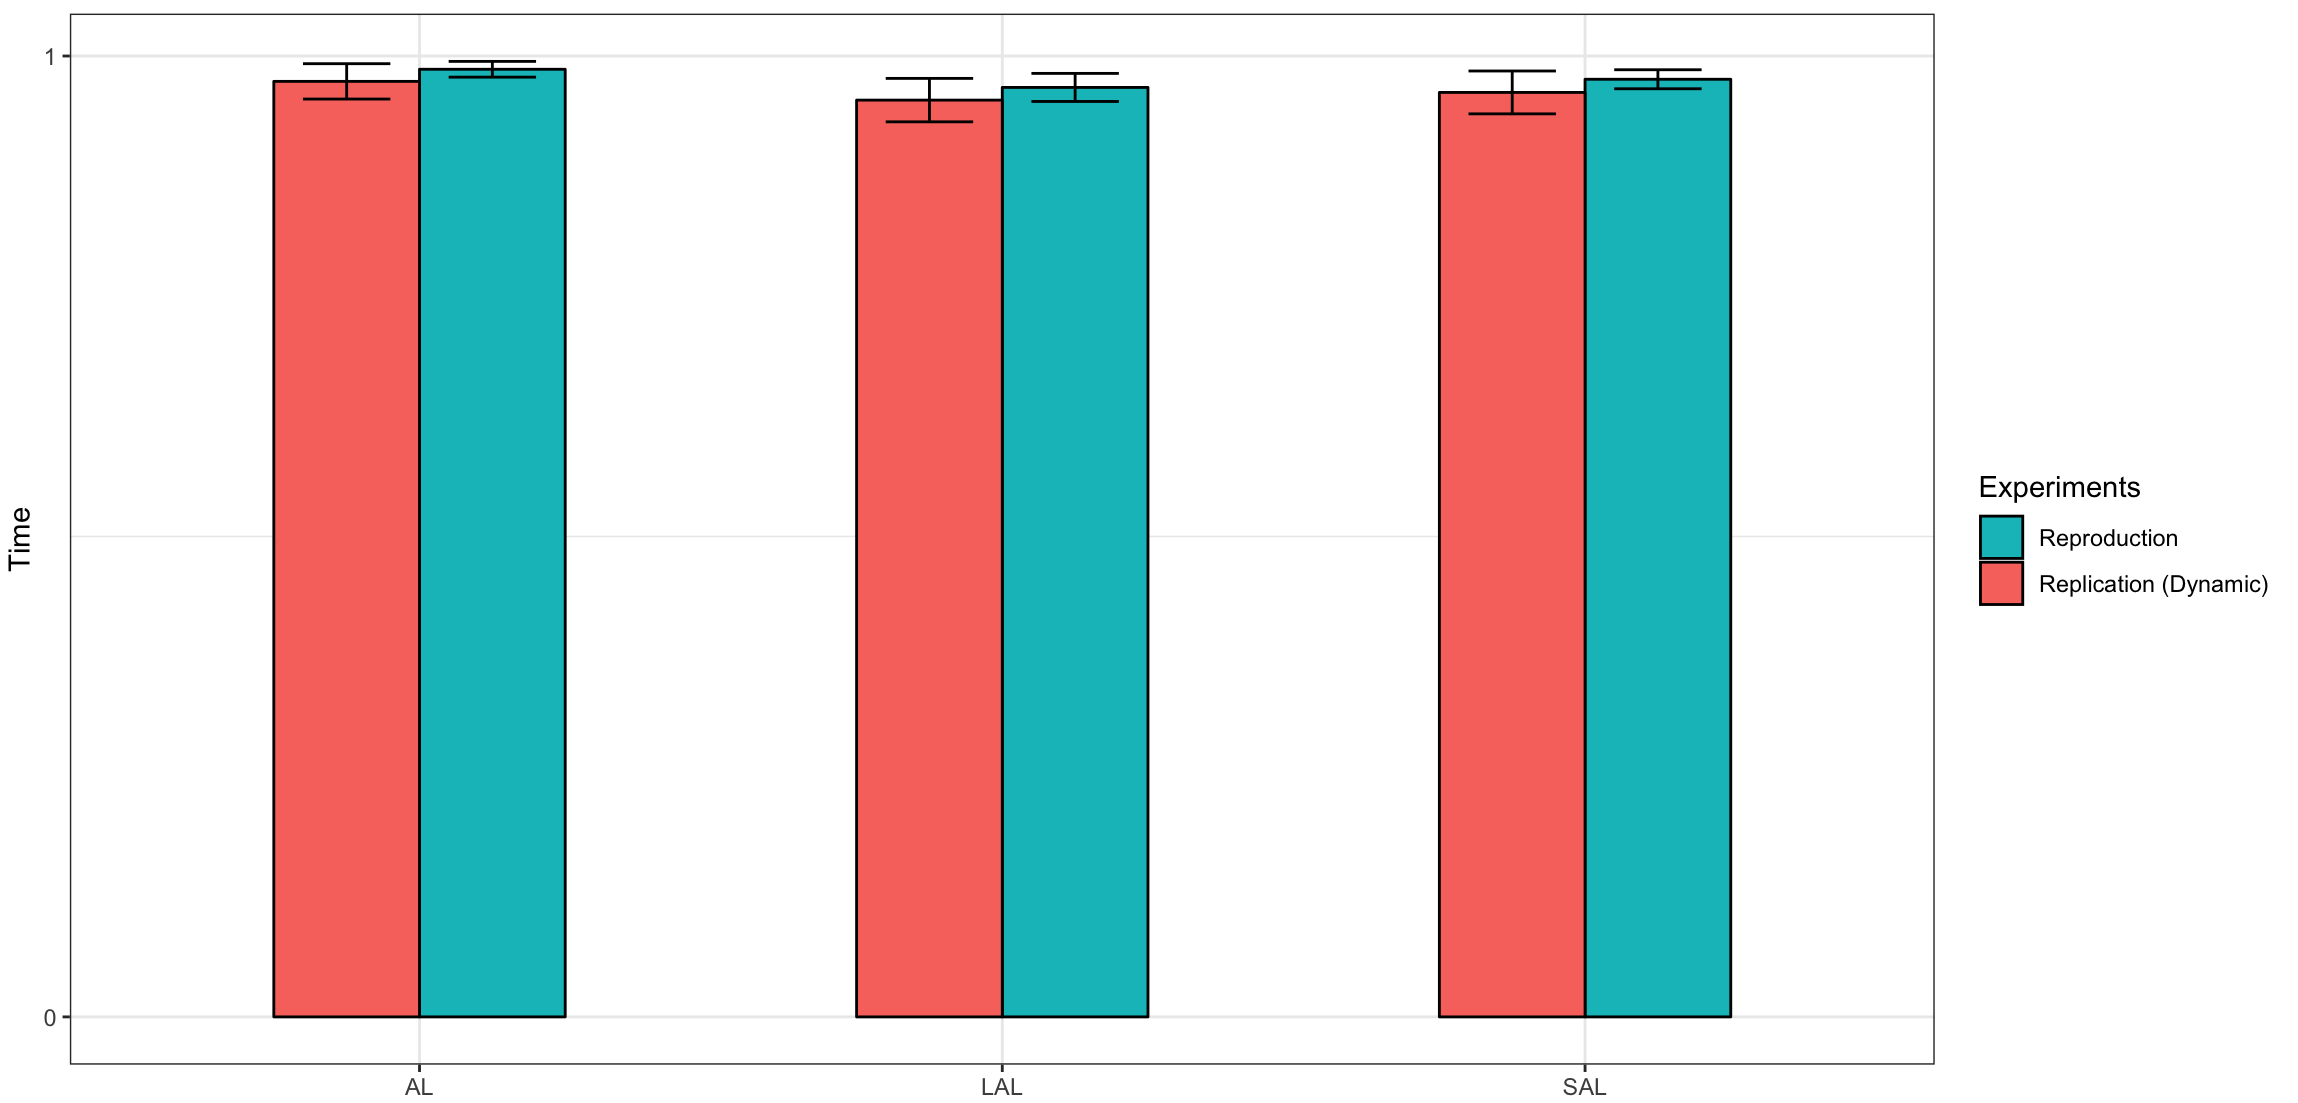
\includegraphics[scale=0.15]{fig/time_orig.png}
		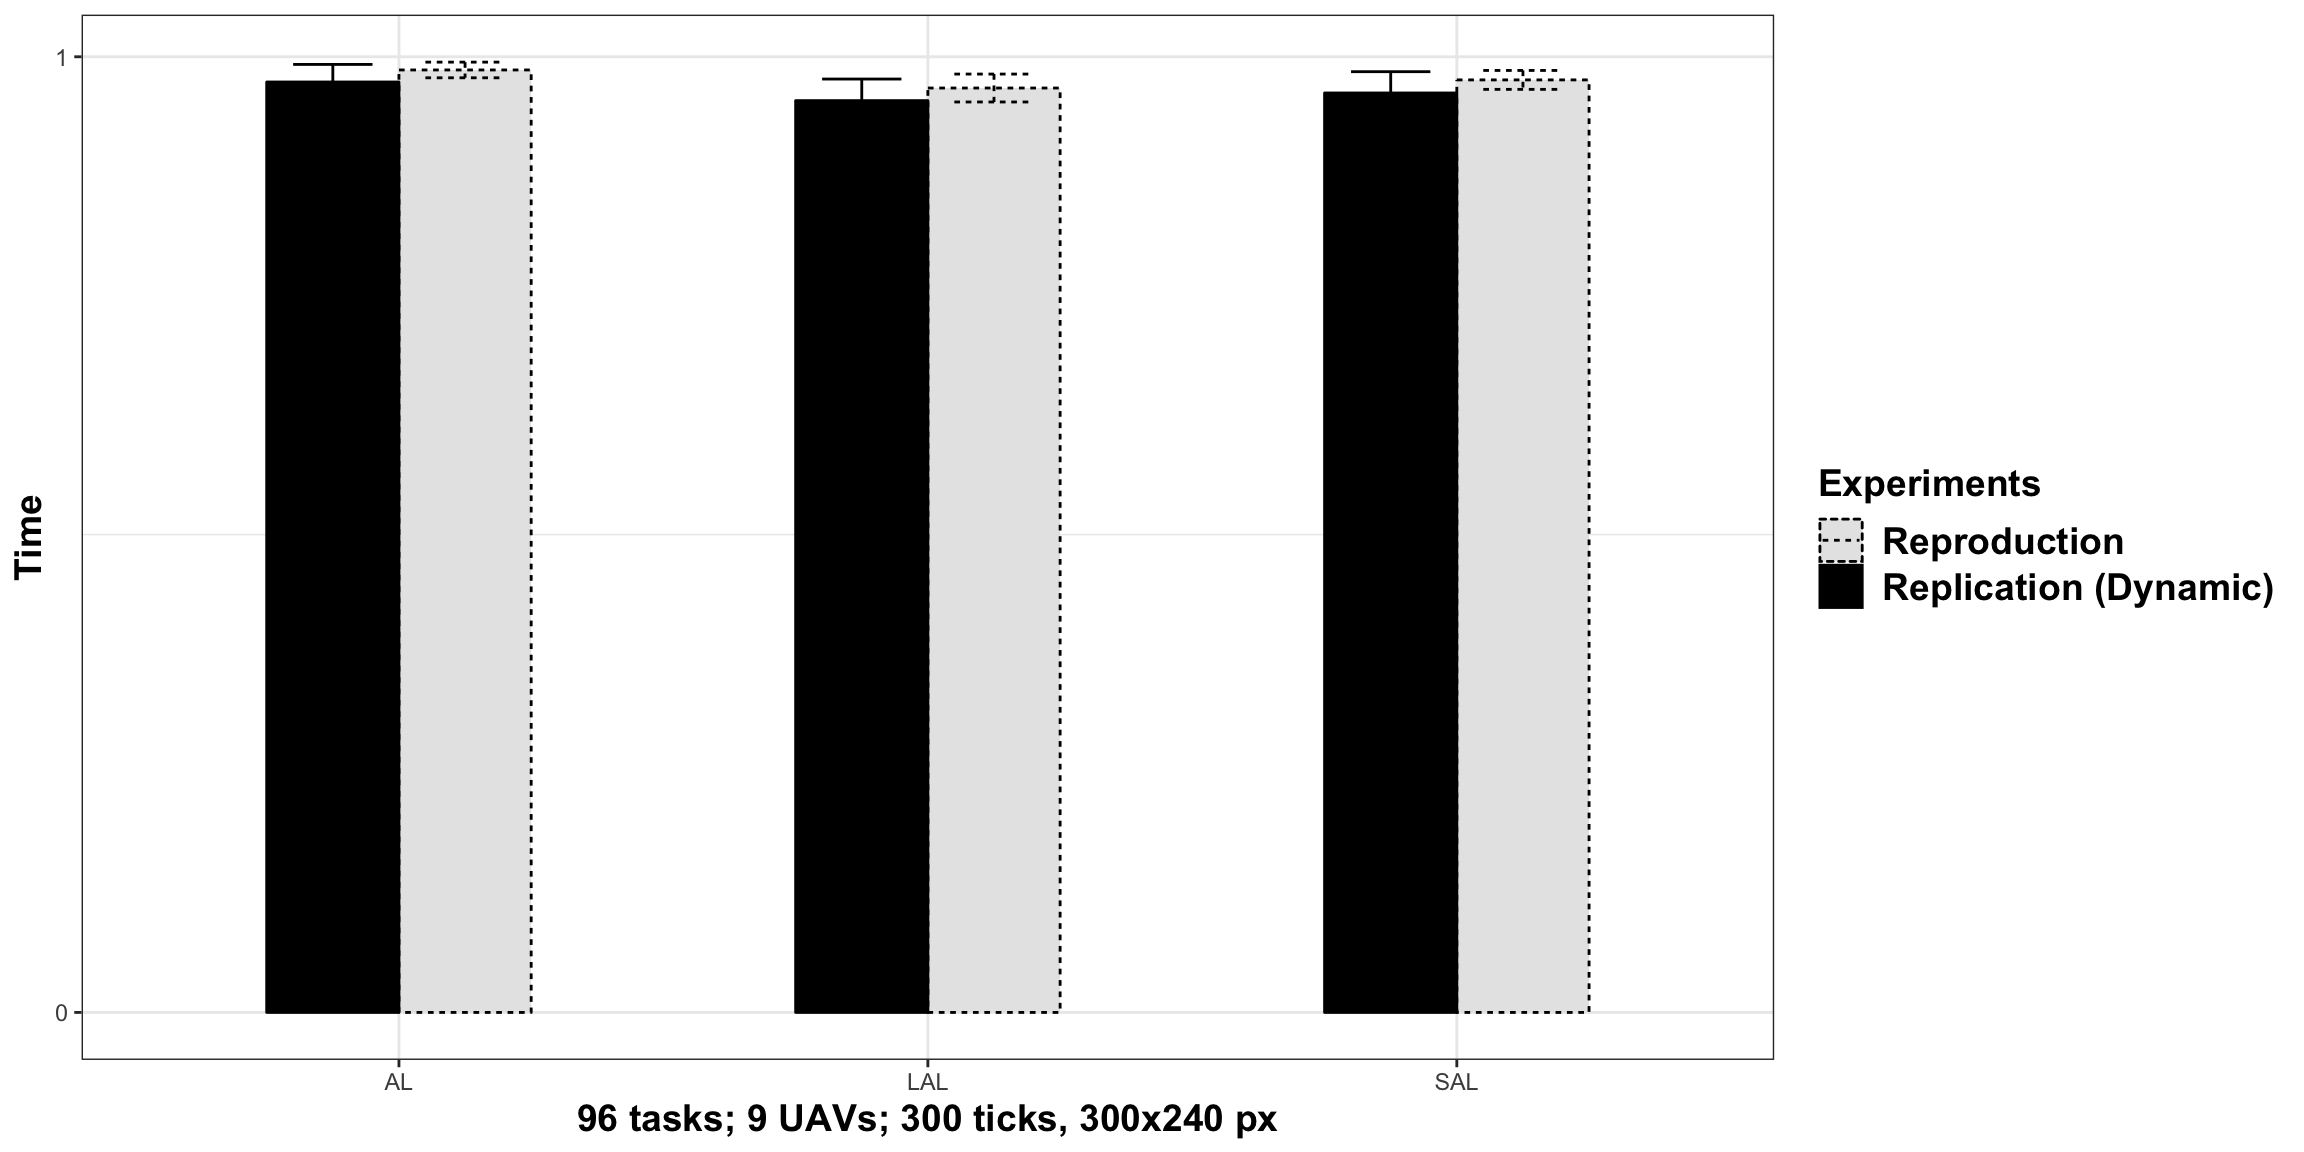
\includegraphics[scale=0.15]{fig/GRAPH05.png}
		\caption{Elapsed Time (96 tasks; 9 UAVs; 300 x 240; 300 ticks)}
		\label{fig:time}
	\end{center}
\end{figure}

The time measurement was done in percentage of total mission time (in ticks) utilization. The result obtained was equivalent to the original study experiments, considering the standard deviation (see Figure \ref{fig:time}). It is explained because the dynamic scenario ensures at least one UAV and this agent spends the most of the available time (in ticks) to execute the tasks allocated to it.

According to what was presented in \cite{MAS07} and \cite{ferreira2007swarm}, the more suitable value for $stimulus$ parameter is $0.6$. However, during the replications, different values were investigated. The resulting differences were not significant compared to those using the original $stimulus$ value in a static context reproduction. Therefore, all final results obtained in this section were based on the $stimulus = 0.6$

\subsection{Second Replication}\label{sec:replication}
The second independent replication was done with the extended algorithms (AL, SAL and LAL) previously presented in Section \ref{sec:changes}. The assessment was done in the same dynamic context used by the first replication (Section \ref{sec:original}), following similar original algorithms conditions and variables values.

Table \ref{table:table06} shows the total reward obtained with the completed tasks, the elapsed time to perform the tasks, then number of completed tasks, the quality obtained with the completed tasks, and the total number of tokens sent with 100 executions and the same \textit{stimulus} and sensors quality used by the original experiments in all scenarios listed in Section \ref{sec:reproducibility}. 

\begin{table}%[ht]
	\small
	\fontsize{6}{6}\selectfont
	\centering
	\caption{Total reward, elapsed time, quantity and quality of the completed tasks and number of exchanged messages for 100 runs of each algorithm after modification, described in Section \ref{sec:changes}}
	\label{table:table06}
	
	\begin{tabular}{rrrrr} \hline
		& AL
		& SAL
		& LAL \\ \hline 
		
		& Mean (St.Dev.)  & Mean (St.Dev.)  & Mean (St.Dev.)  \\ [1ex]
		
		\multicolumn{5}{l}{\textbf{$\longrightarrow$ 3 UAVs and 4 tasks in the area of 100x80 pixels with deadline of 300 ticks }} \\
	Total reward           & 2.0608   ($\pm$0.4417)  &  2.1512  ($\pm$0.3328) & 2.2684  ($\pm$0.2372)   \\
	Elapsed time (norm)    & 0.4147   ($\pm$0.1358)  &  0.4085  ($\pm$0.1422) & 0.3506  ($\pm$0.1159)    \\ 
	Comp. tasks (norm)     & 0.9875   ($\pm$0.0548)  &  0.9975  ($\pm$0.0250) & 0.9975  ($\pm$0.0250)    \\ 
	Quality (norm)         & 0.8218   ($\pm$0.1747)  &  0.8437  ($\pm$0.1434) & 0.9215  ($\pm$0.1115)   \\ 
	Sending token          &  5.0800  ($\pm$2.3471)  &  5.3000  ($\pm$2.8972) & 7.0300  ($\pm$2.3632)   \\ [1ex]
		
		\multicolumn{5}{l}{\textbf{$\longrightarrow$ 3 UAVs and 8 tasks in the area of 100x80 pixels with deadline of 300 ticks}} \\
	Total reward           & 3.2771   ($\pm$0.5984)  &  3.4573  ($\pm$0.5436) & 3.7628  ($\pm$0.4796)   \\
	Elapsed time (norm)    & 0.6927   ($\pm$0.0762)  &  0.7016  ($\pm$0.0895) & 0.6714  ($\pm$0.0642)    \\ 
	Comp. tasks (norm)     & 0.8538   ($\pm$0.1006)  &  0.8475  ($\pm$0.1060) & 0.8888  ($\pm$0.0886)    \\ 
	Quality (norm)         & 0.7151  ($\pm$0.1218)   &  0.7494  ($\pm$0.1399) & 0.8047  ($\pm$0.0978)  \\ 
	Sending token          & 10.6100 ($\pm$2.5222)   & 10.1900  ($\pm$2.9566) & 14.7600 ($\pm$2.8467)  \\ [1ex]
	
	    \multicolumn{5}{l}{\textbf{$\longrightarrow$ 3 UAVs and 16 tasks in the area of 100x80 pixels with deadline of 300 ticks}} \\
	Total reward           & 4.6678   ($\pm$0.9381)  &  6.8921  ($\pm$0.9166) & 7.8121  ($\pm$0.7524)   \\
	Elapsed time (norm)    & 0.7393   ($\pm$0.0720)  &  0.7575  ($\pm$0.0658) & 0.7510  ($\pm$0.0720)    \\ 
	Comp. tasks (norm)     & 0.5131   ($\pm$0.0723)  &  0.6113  ($\pm$0.0600) & 0.6500  ($\pm$0.0526)    \\ 
	Quality (norm)         & 0.7505  ($\pm$0.1290)   &  0.8813  ($\pm$0.0902) & 0.9532  ($\pm$0.0505)  \\ 
	Sending token          & 9.7600  ($\pm$2.4000)   & 10.1700  ($\pm$2.2699) & 25.7400 ($\pm$3.4160)  \\ [1ex]
	
	    \multicolumn{5}{l}{\textbf{$\longrightarrow$  3 UAVs and 32 tasks in the area of 100x80 pixels with deadline of 300 ticks}} \\
	Total reward           & 4.7568   ($\pm$1.1019)  & 10.0601  ($\pm$0.9066) & 11.0194 ($\pm$0.7653)   \\
	Elapsed time (norm)    & 0.7512   ($\pm$0.0692)  &  0.7343  ($\pm$0.0558) & 0.7271  ($\pm$0.0538)    \\ 
	Comp. tasks (norm)     & 0.2563   ($\pm$0.0433)  &  0.3906  ($\pm$0.0340) & 0.4063  ($\pm$0.0291)    \\ 
	Quality (norm)         & 0.7134  ($\pm$0.1094)   &  0.9502  ($\pm$0.0479) & 0.9742  ($\pm$0.0269)  \\ 
	Sending token          & 6.8900  ($\pm$1.1712)   &  7.0600  ($\pm$1.2045) & 32.1500 ($\pm$1.8607)  \\ [1ex]
	
	    \multicolumn{5}{l}{\textbf{$\longrightarrow$ 6 UAVs and 64 tasks in the area of 200x160 pixels with deadline of 300 ticks}} \\
	Total reward           & 5.1439   ($\pm$1.2455)  & 16.3631  ($\pm$1.2697) & 13.5601 ($\pm$0.9898)   \\
	Elapsed time (norm)    & 0.8836   ($\pm$0.0836)  &  0.8331  ($\pm$0.0669) & 0.8100  ($\pm$0.0733)    \\ 
	Comp. tasks (norm)     & 0.1231   ($\pm$0.0245)  &  0.2763  ($\pm$0.0202) & 0.2993  ($\pm$0.0213)    \\ 
	Quality (norm)         & 0.7834  ($\pm$0.1374)   &  0.9919  ($\pm$0.0185) & 0.9968  ($\pm$0.0127)  \\ 
	Sending token          & 22.4000 ($\pm$1.3559)   & 22.1300  ($\pm$1.3154) & 95.2100 ($\pm$3.5142)  \\ [1ex]

        \multicolumn{5}{l}{\textbf{$\longrightarrow$ 9 UAVs and 96 tasks in the area of 300x240 pixels with deadline of 300 ticks}} \\
	Total reward           & 4.9713   ($\pm$1.4175)  & 15.6611  ($\pm$1.7195) & 18.2397 ($\pm$1.8068)   \\
	Elapsed time (norm)    & 0.9355   ($\pm$0.0683)  &  0.9143  ($\pm$0.0534) & 0.9067  ($\pm$0.0643)    \\ 
	Comp. tasks (norm)     & 0.0773   ($\pm$0.0175)  &  0.1741  ($\pm$0.0182) & 0.1993  ($\pm$0.0193)    \\ 
	Quality (norm)         & 0.7932   ($\pm$0.1053)  &  0.9980  ($\pm$0.0083) & 0.9993  ($\pm$0.0040)   \\ 
	Sending token          & 47.9600  ($\pm$1.9012)  &  48.0200 ($\pm$2.0100) & 148.6200($\pm$4.8550)   \\ [1ex]

		\hline
	\end{tabular}
\end{table} 






The results obtained by these modified algorithms, with small number of UAVs(3) and tasks (4, 8 and 16), presented less difference from the original algorithms in the dynamic scenario (Section \ref{sec:original}). As the number of elements is low, the differences are within the standard deviation. Therefore, in the following, the largest group (9 UAVs and 96 tasks) was used to explore the differences in the results. 

Overall, the data from Table \ref{table:table06} show that after the modifications described in Section \ref{sec:changes}, resulting in extended algorithms, different results were obtained  compared with the original ones in the dynamic scenario. From all assessed metrics, quality and number of exchanged messages were those with more significant variation.

In particular, the number of messages increases over 100\% with the modified algorithms, indicating a communication overhead. The exchanged messages in the original and the modified algorithms are depicted in Figure \ref{fig:fig06}. This overhead can be explained by the token reset made in the modified algorithms (see Line~\ref{line:step2_begin} in Algorithm \ref{algo:change}). Resetting the token allows it to run more often among the UAVs, generating more messages exchanged among these elements.

\begin{figure}[h!]
	\begin{center}
		%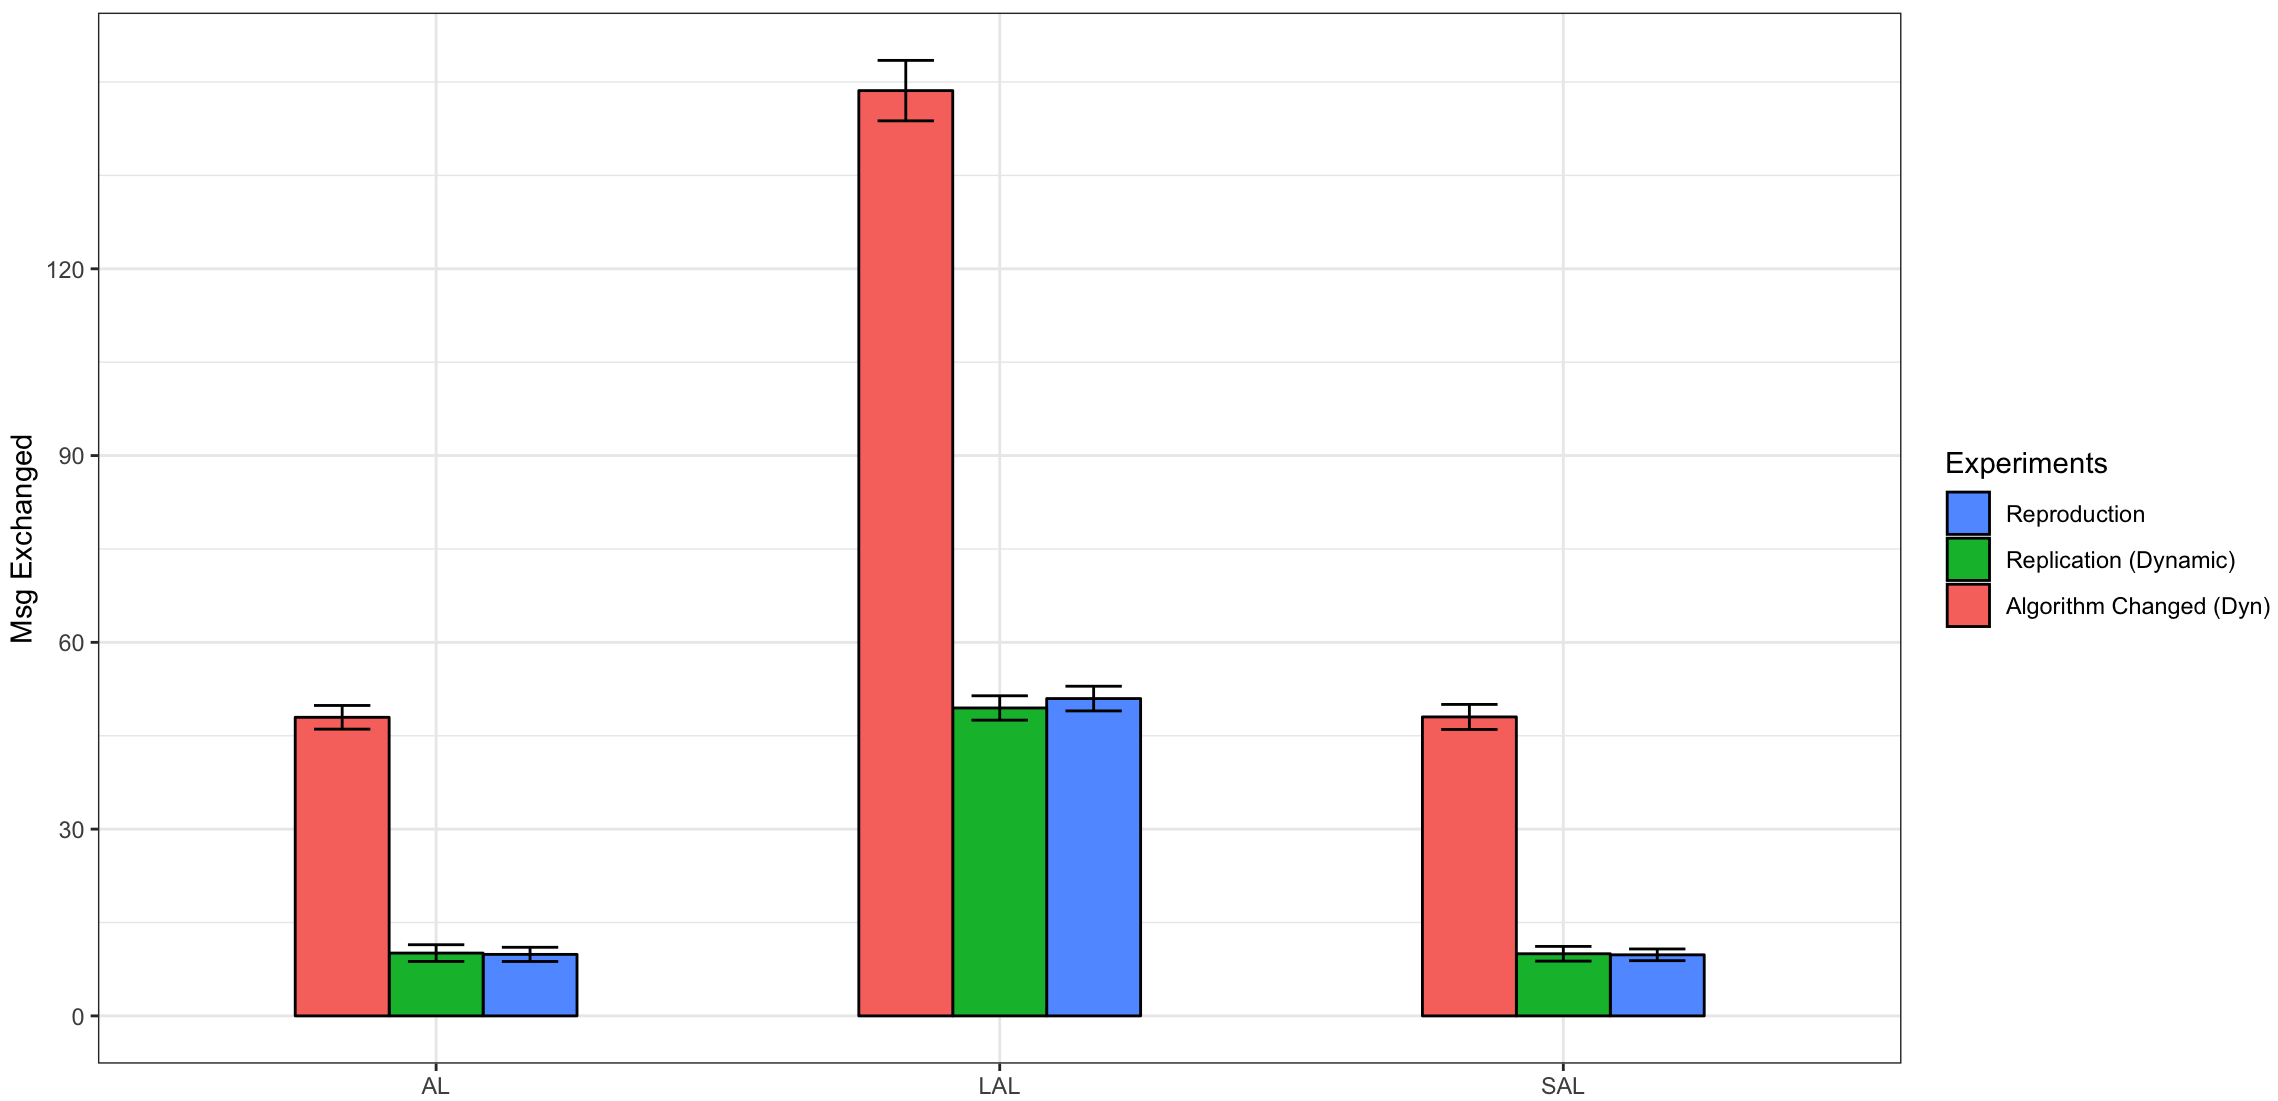
\includegraphics[scale=0.15]{fig/fig06.png}
		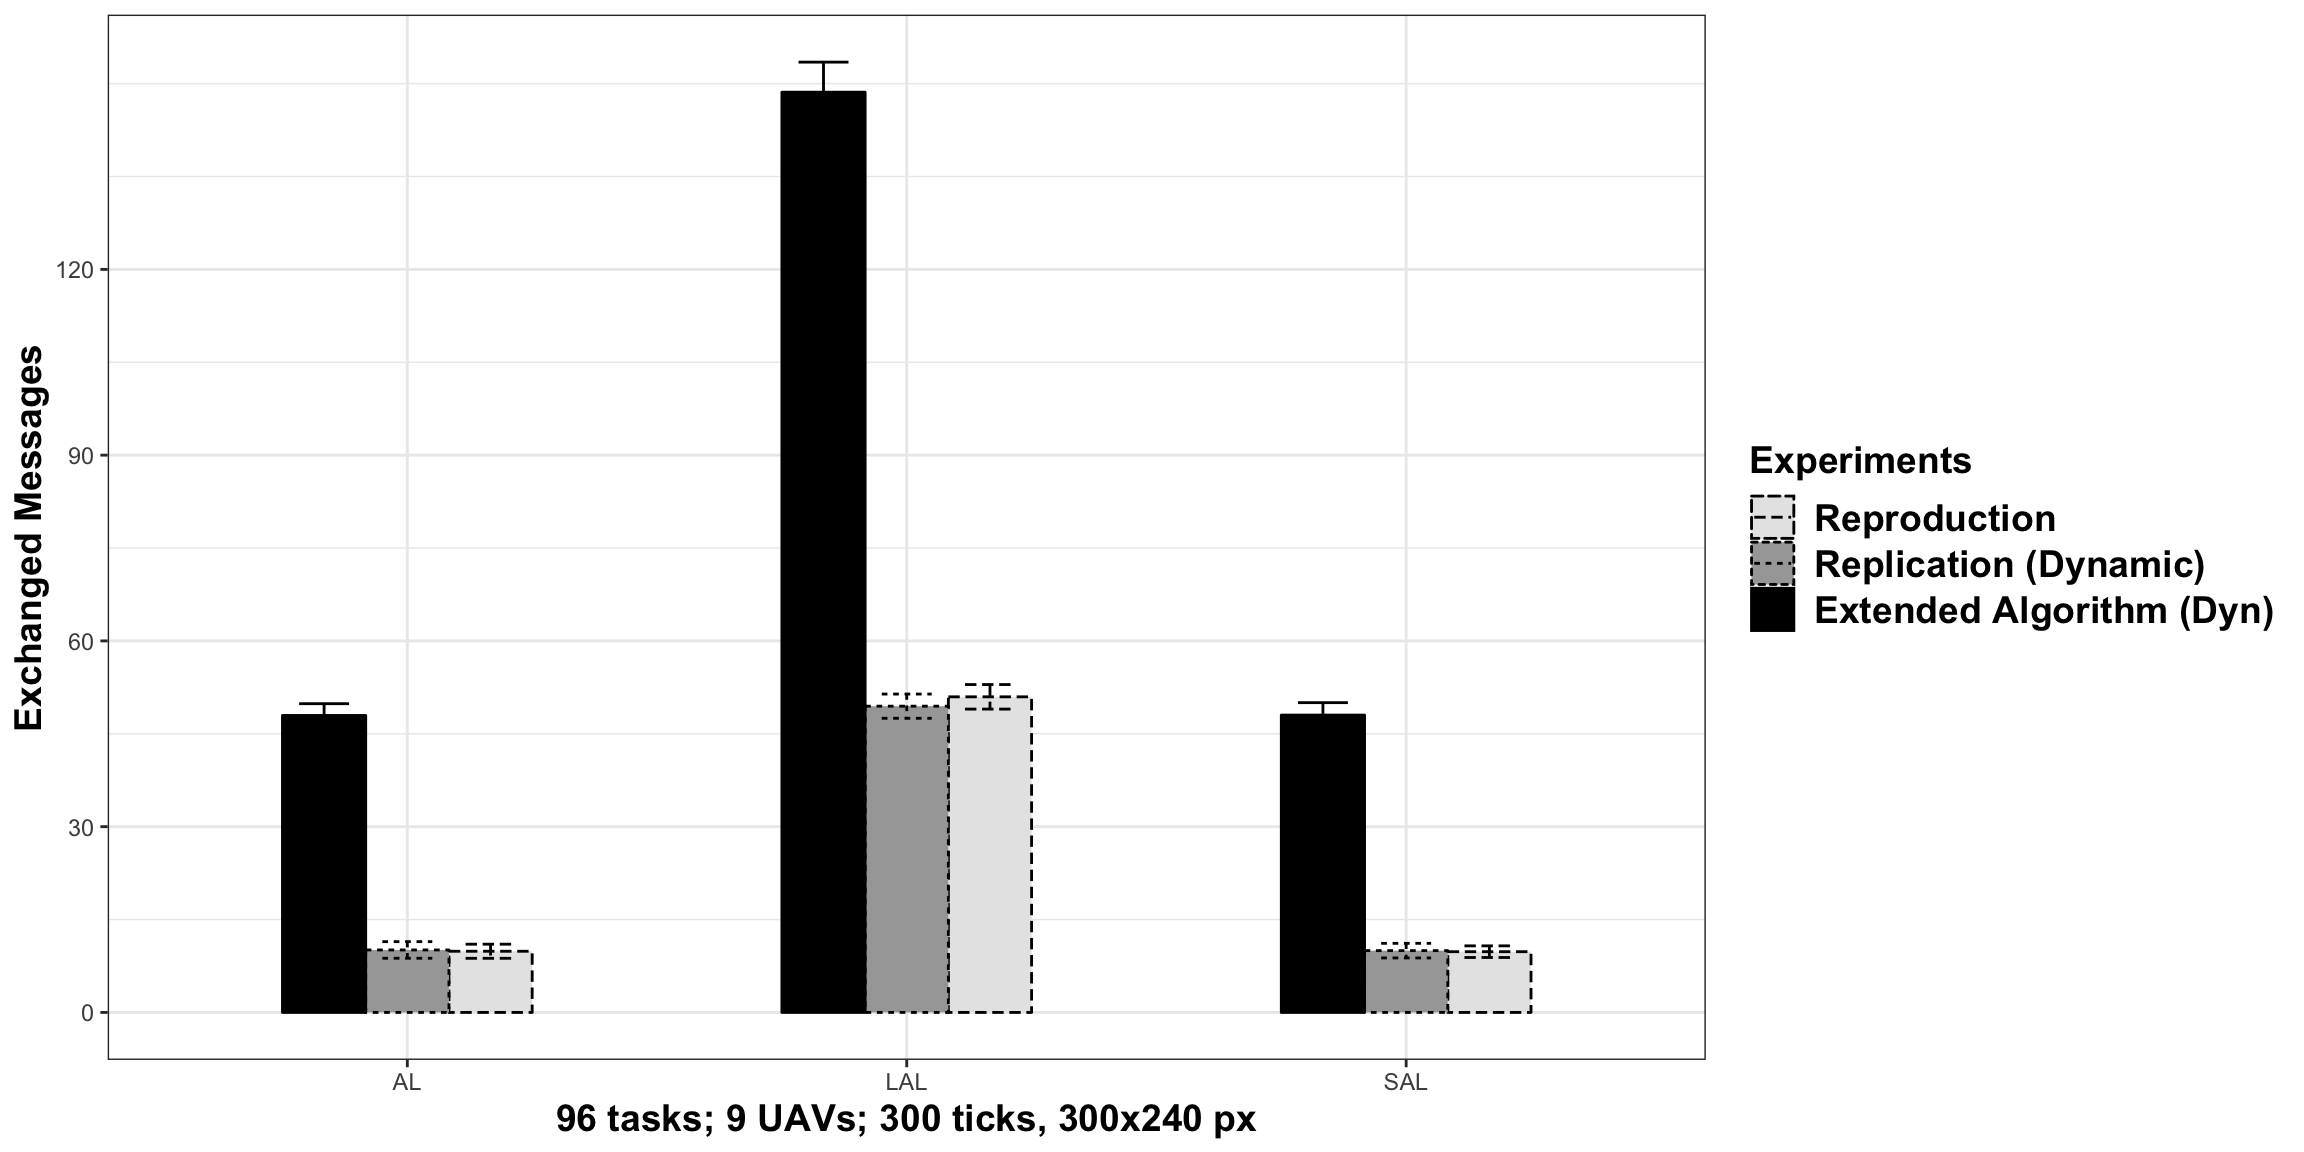
\includegraphics[scale=0.15]{fig/GRAPH06.png}
		\caption{Exchanged messages  of the original algorithm in the static scenario (reproduction), in the dynamic scenario (replication) and the modified algorithms in dynamic scenario (96 tasks; 9 UAVs; 300 x 240; 300 ticks)}
		\label{fig:fig06}
	\end{center}
\end{figure}



Figure \ref{fig:fig05} shows that the extended algorithms presented an increase of around 40\% in the quality attribute compared with what was obtained in the first replication (Section \ref{sec:original}). This recovering was due to the task redistribution with the token reset after a context change with a UAV removed from the team. The new token round through the UAVs ensures reallocating tasks to maximize the quality results, relating the task with the agent that has the best sensor to perform it.

\begin{figure}[h!]
	\begin{center}
		%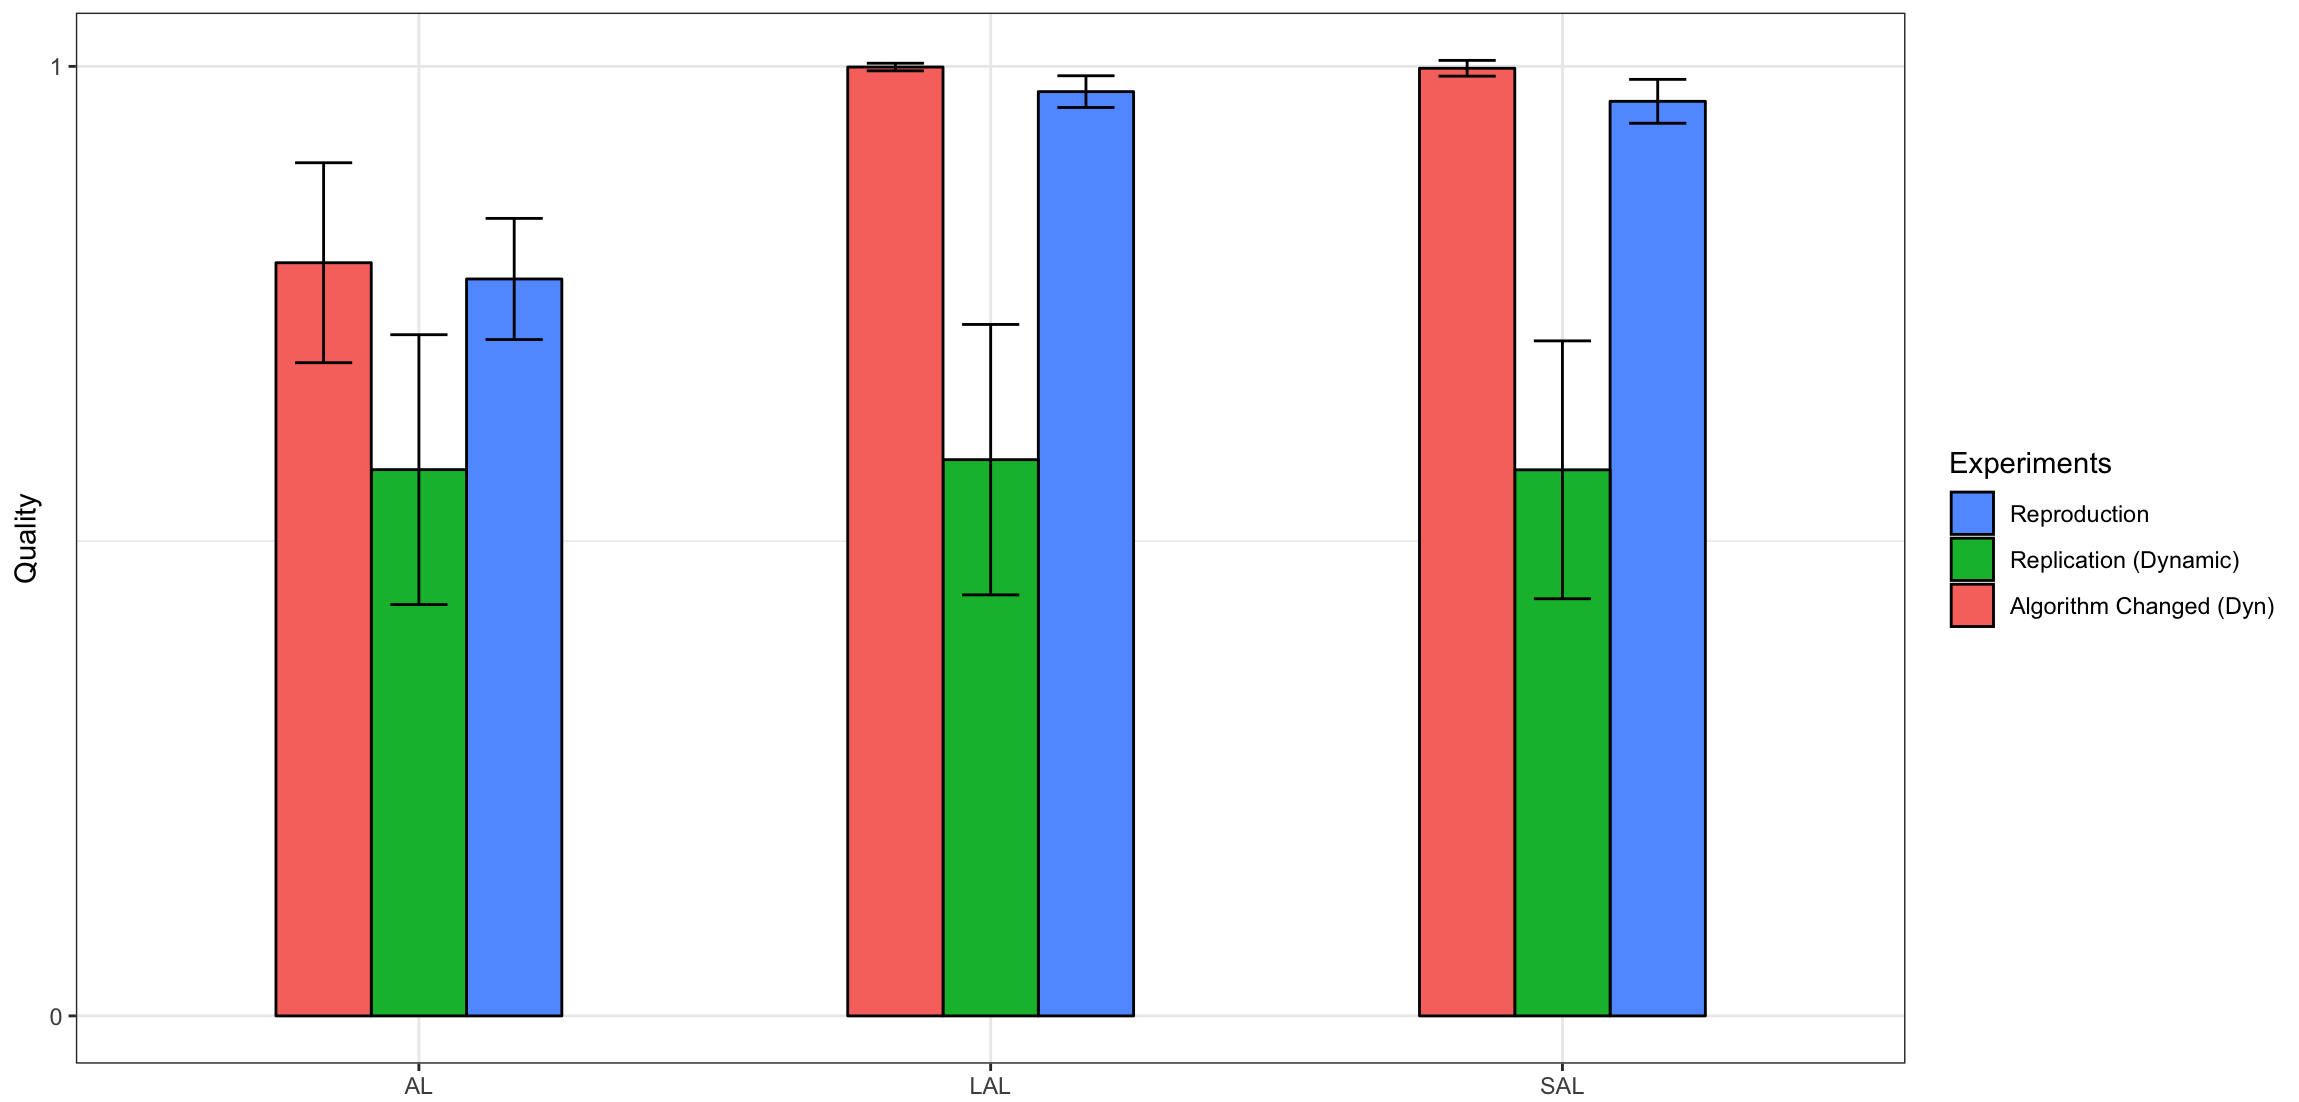
\includegraphics[scale=0.15]{fig/fig05.png}
		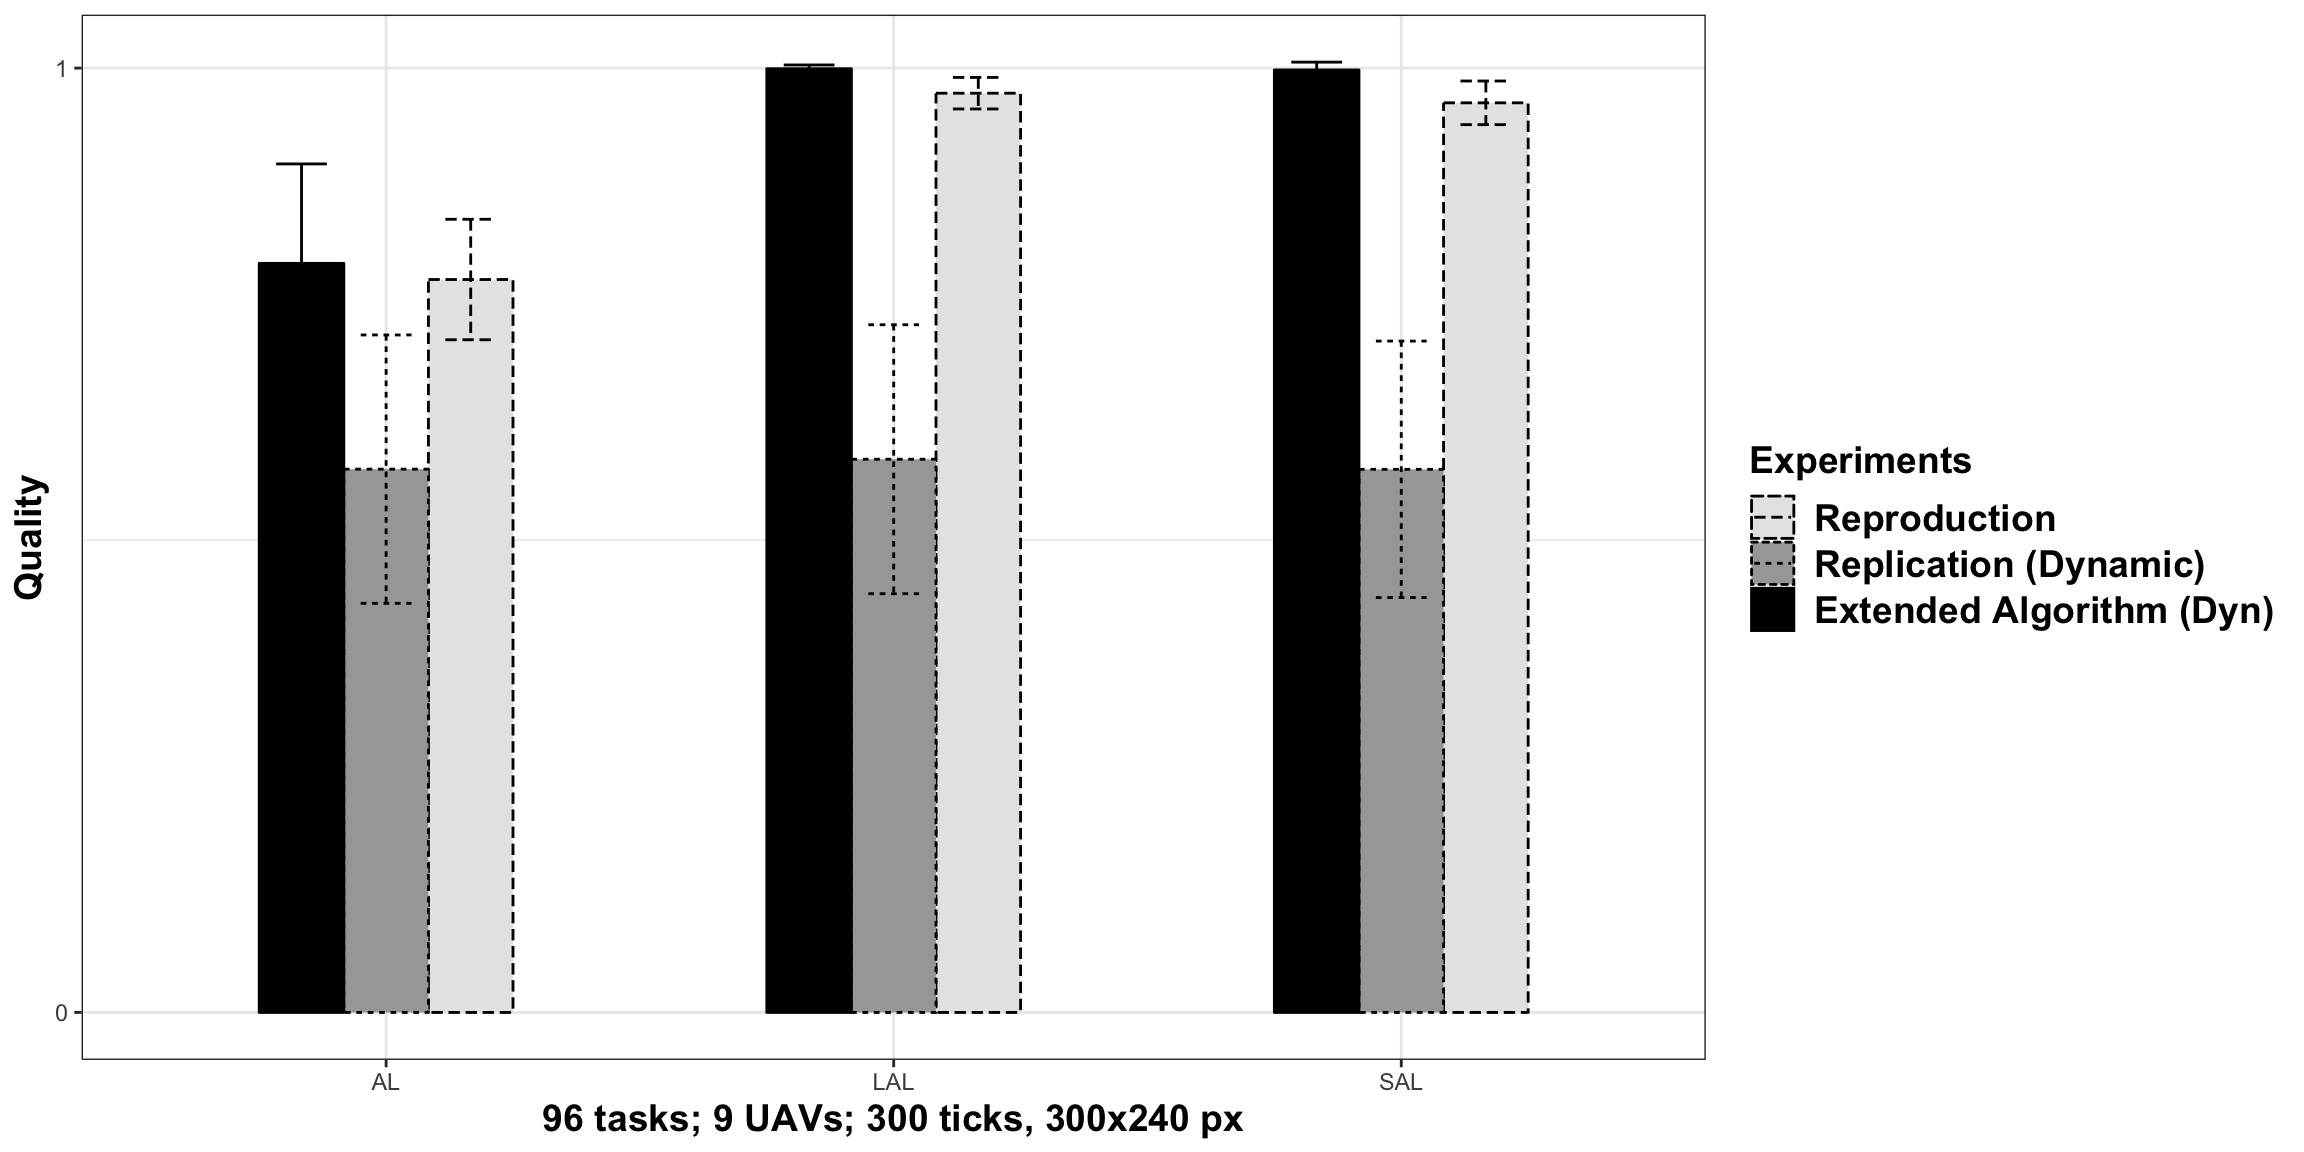
\includegraphics[scale=0.15]{fig/GRAPH07.png}
		\caption{Quality of the original algorithm in the static scenario (reproduction), in the dynamic scenario (replication) and the modified algorithms in dynamic scenario (96 tasks; 9 UAVs; 300 x 240; 300 ticks)}
		\label{fig:fig05}
	\end{center}
\end{figure}

 Figure \ref{fig:din02} shows the elapsed time to perform all tasks allocated to the UAVs. It presented a slight decrease of around 5\% because the agents spend more time communicating and adjusting the tasks allocation in order to optimize the quality. It results in less time available to execute the tasks due to the reallocation. However, the difference among the three algorithms (AL, SAL and LAL) in the dynamic context is within the standard deviation as seen in Figure \ref{fig:din02}.
 
\begin{figure}[h!]
	\begin{center}
		%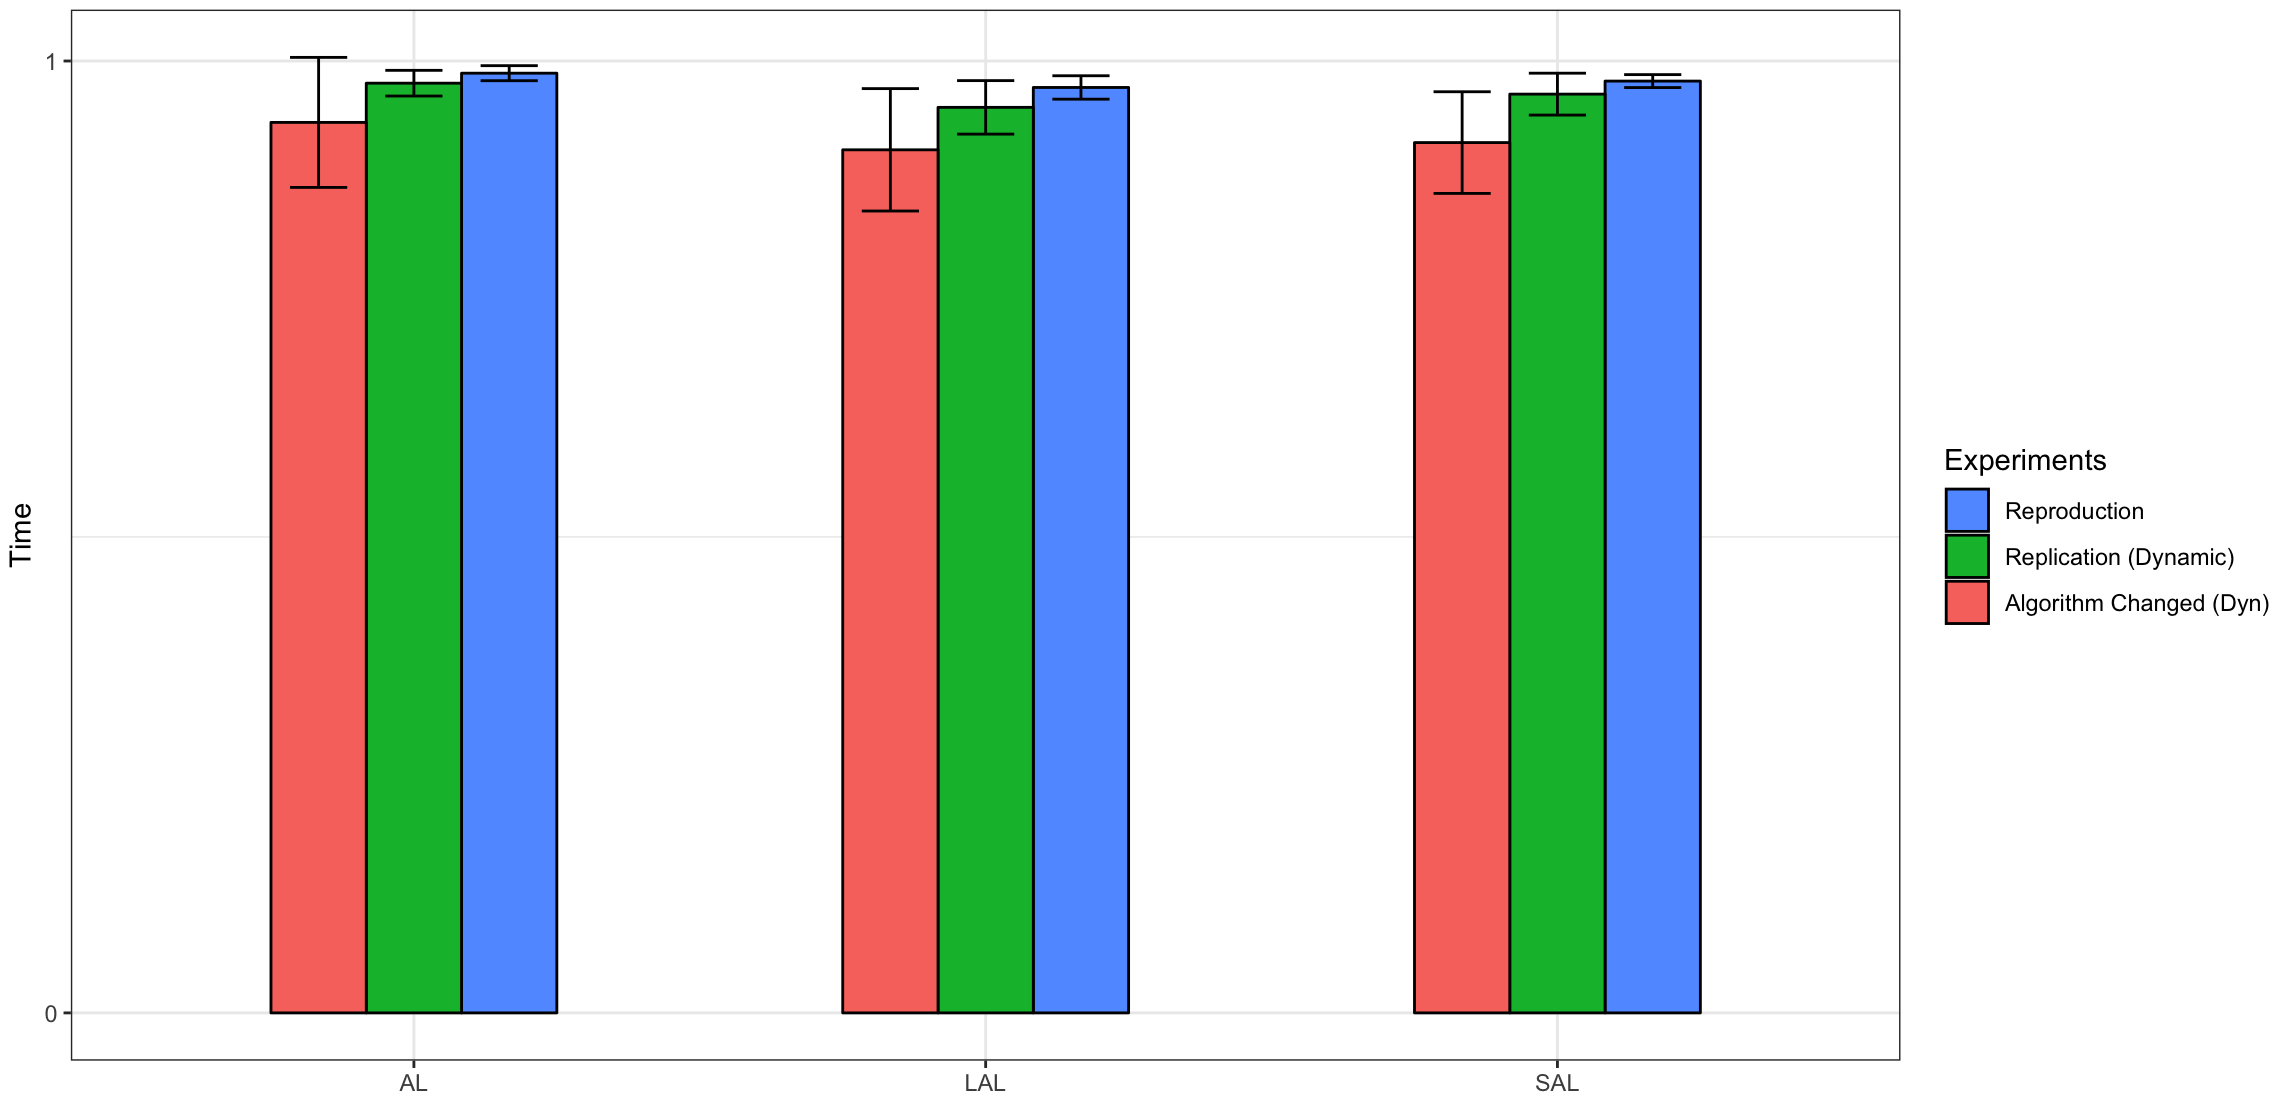
\includegraphics[scale=0.15]{fig/din3.png}
		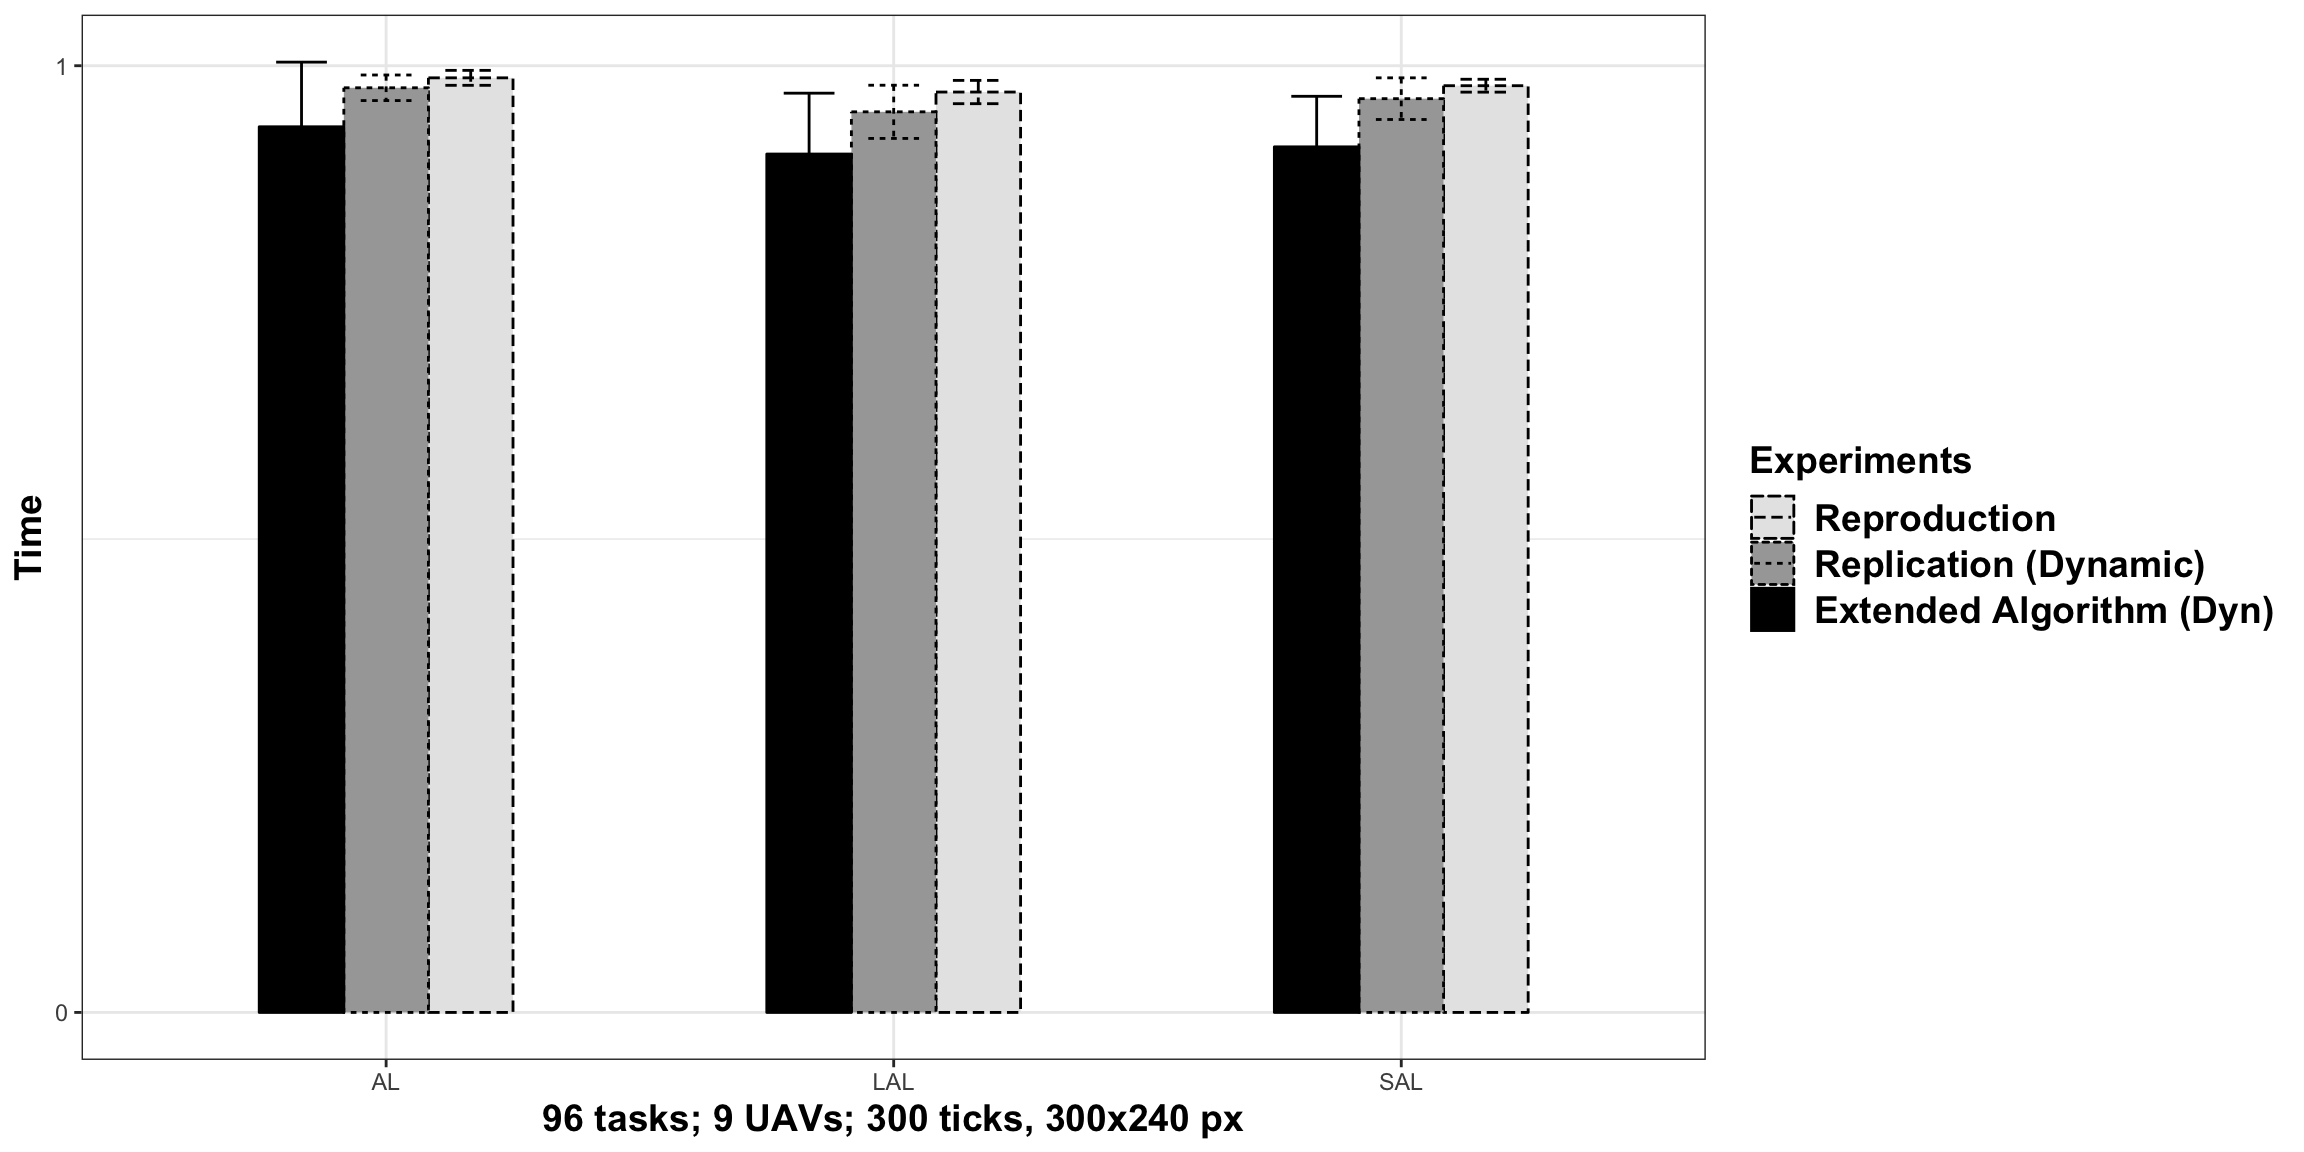
\includegraphics[scale=0.15]{fig/GRAPH08.png}
		\caption{Elapsed Time  in the dynamic scenario (replication) to the original algorithm in static scenario (reproduction), in the dynamic scenario (replication) and the modified ones (96 tasks; 9 UAVs; 300 x 240; 300 ticks)}
		\label{fig:din02}
	\end{center}
\end{figure}

Analyzing the number of finished tasks, depicted in Figure \ref{fig:box01}, it is visible a decrease comparing the algorithms. The lowest one is for the extended algorithms and it occurs because the team spends more time communicating and adjusting the tasks allocation in order to optimize quality thus with less available time for task execution. However, the difference runs into the standard deviation as seen in Figure \ref{fig:box01}.

\begin{figure}[!htb]
\centering
\subfloat{
%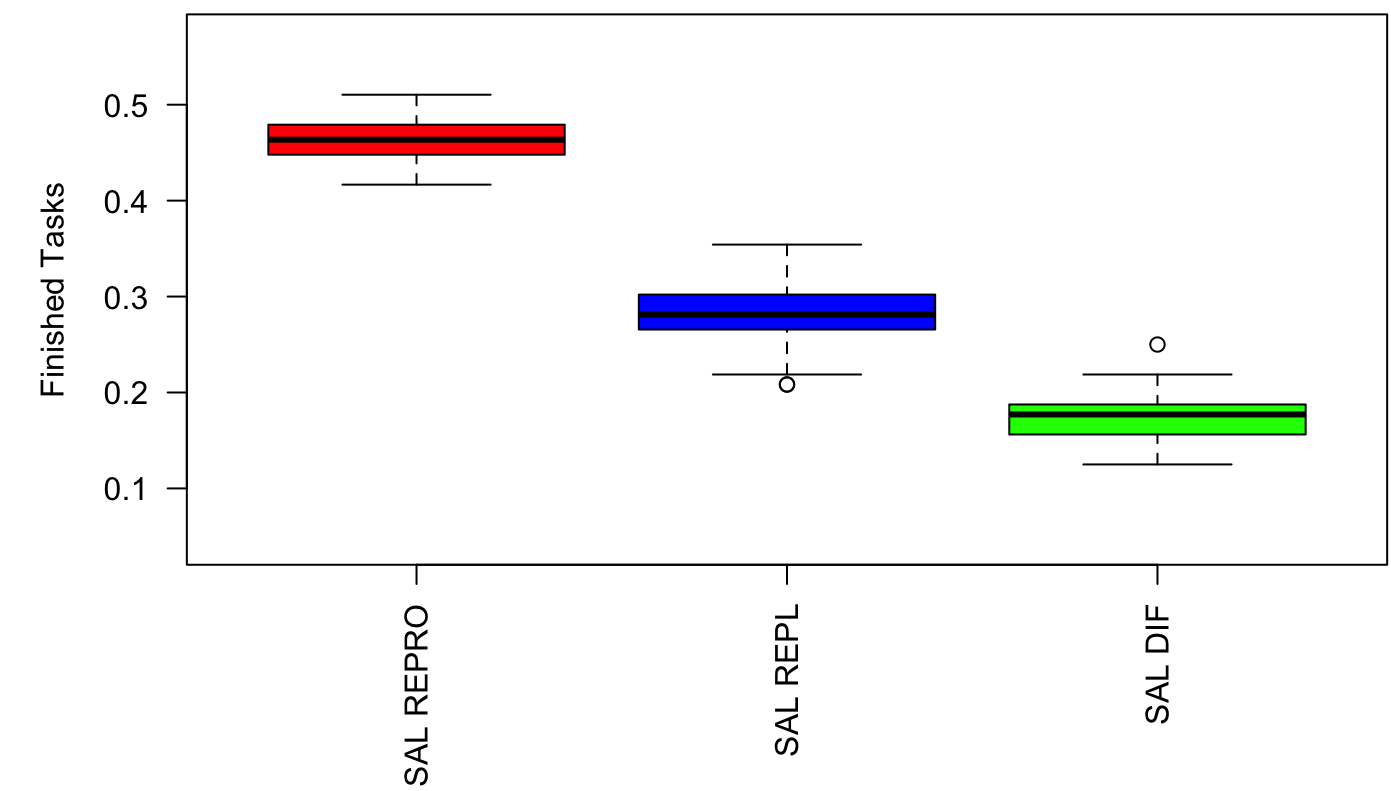
\includegraphics[scale=0.1]{fig/box1.png}
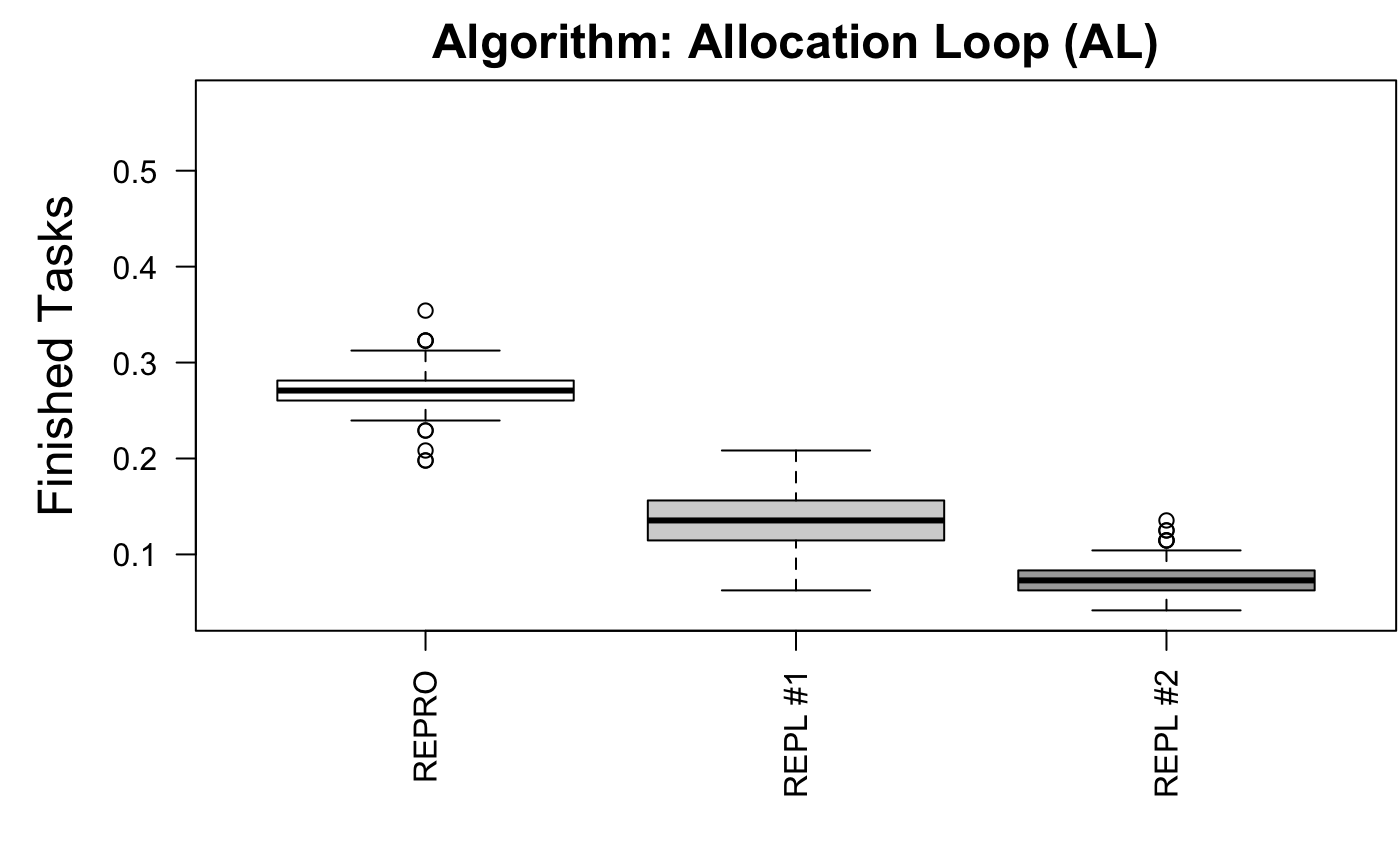
\includegraphics[scale=0.1]{fig/BOX01.png}
}
\quad
\subfloat{
%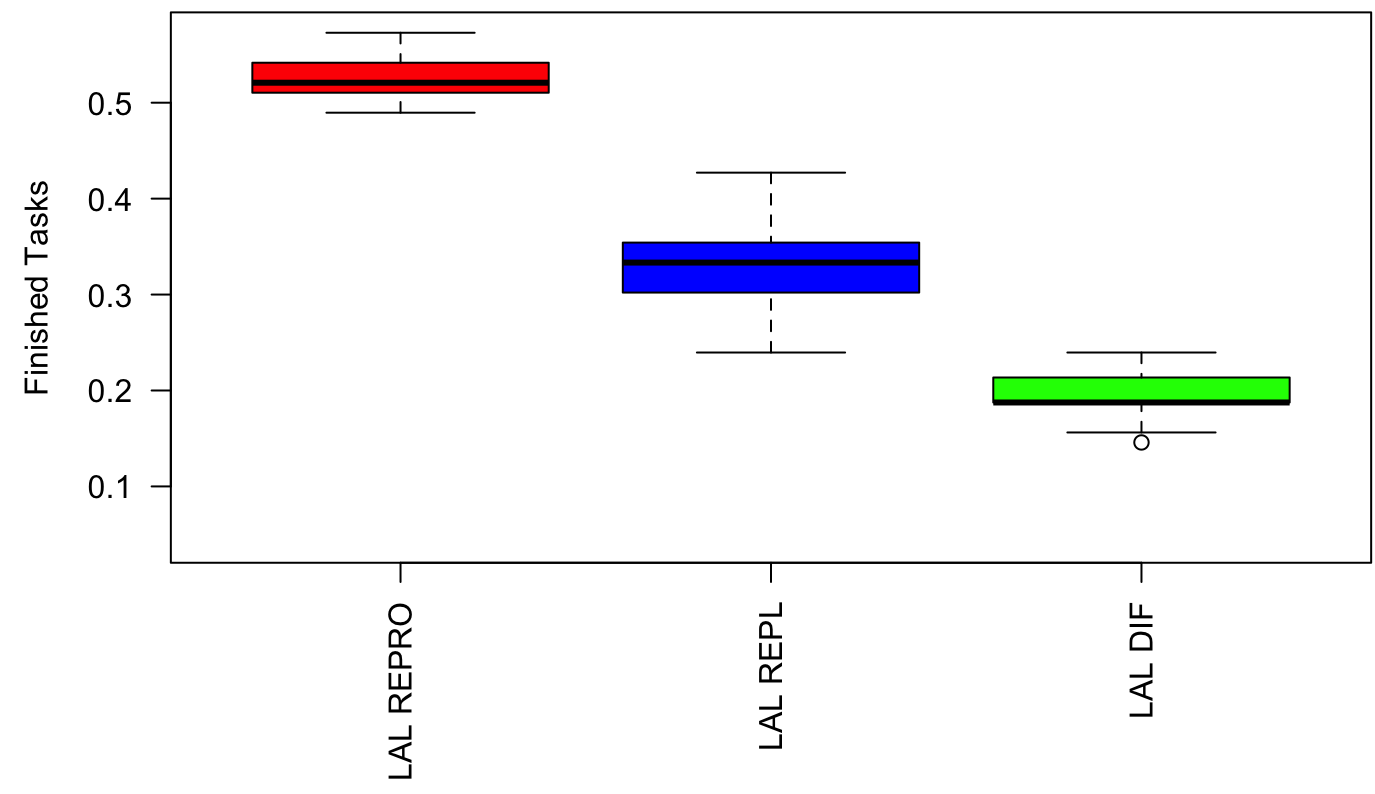
\includegraphics[scale=0.1]{fig/box2.png}
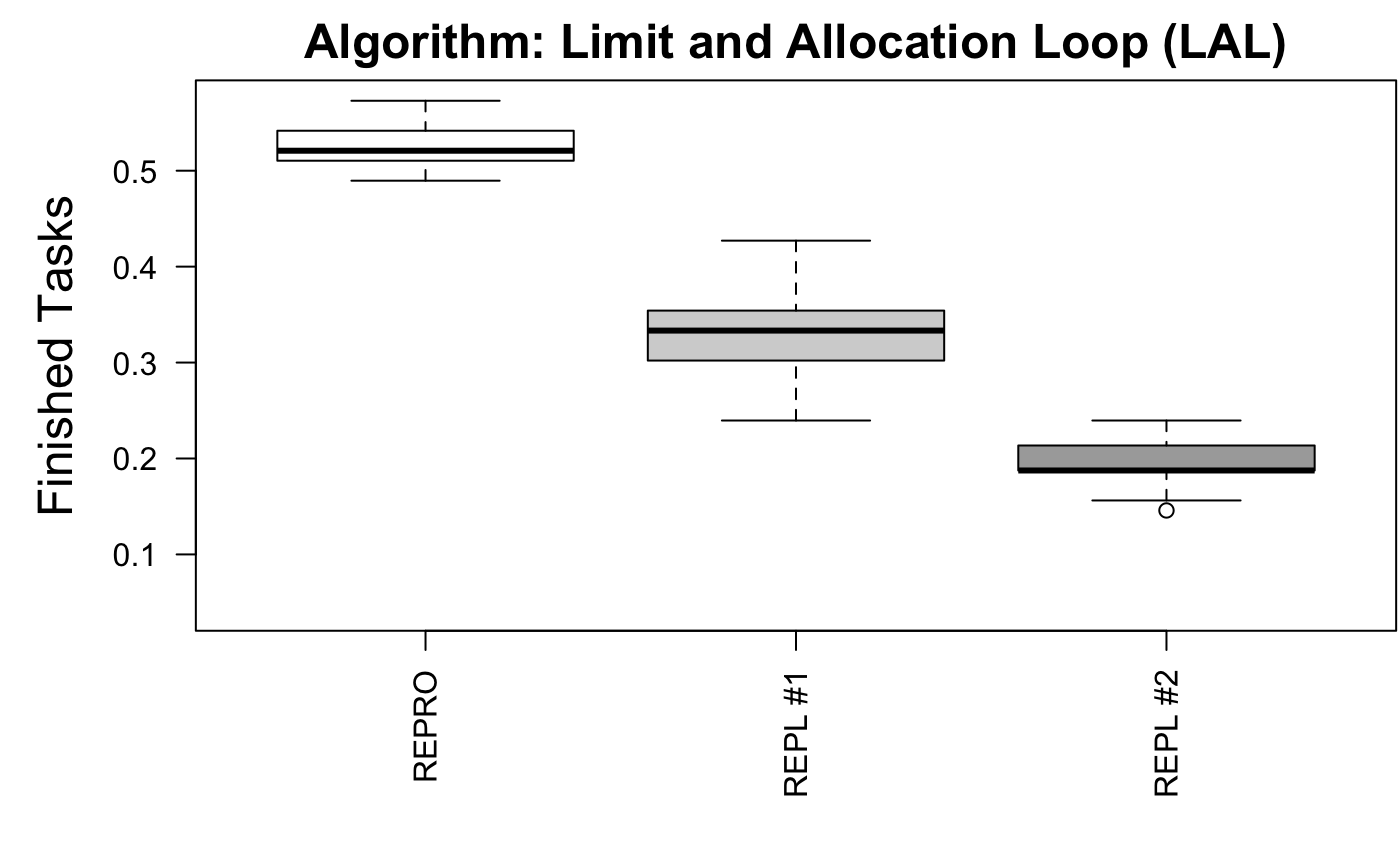
\includegraphics[scale=0.1]{fig/BOX02.png}
}
\quad
\subfloat{
%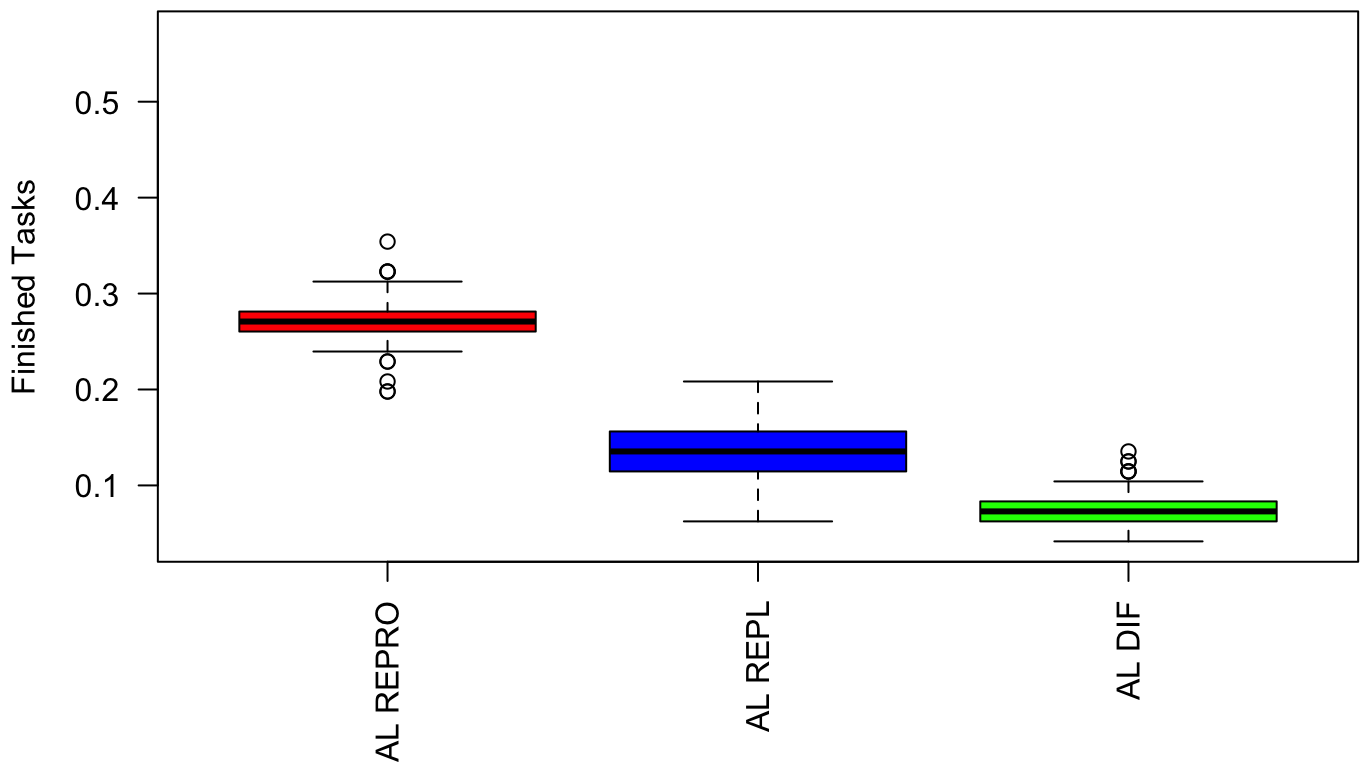
\includegraphics[scale=0.1]{fig/box3.png}
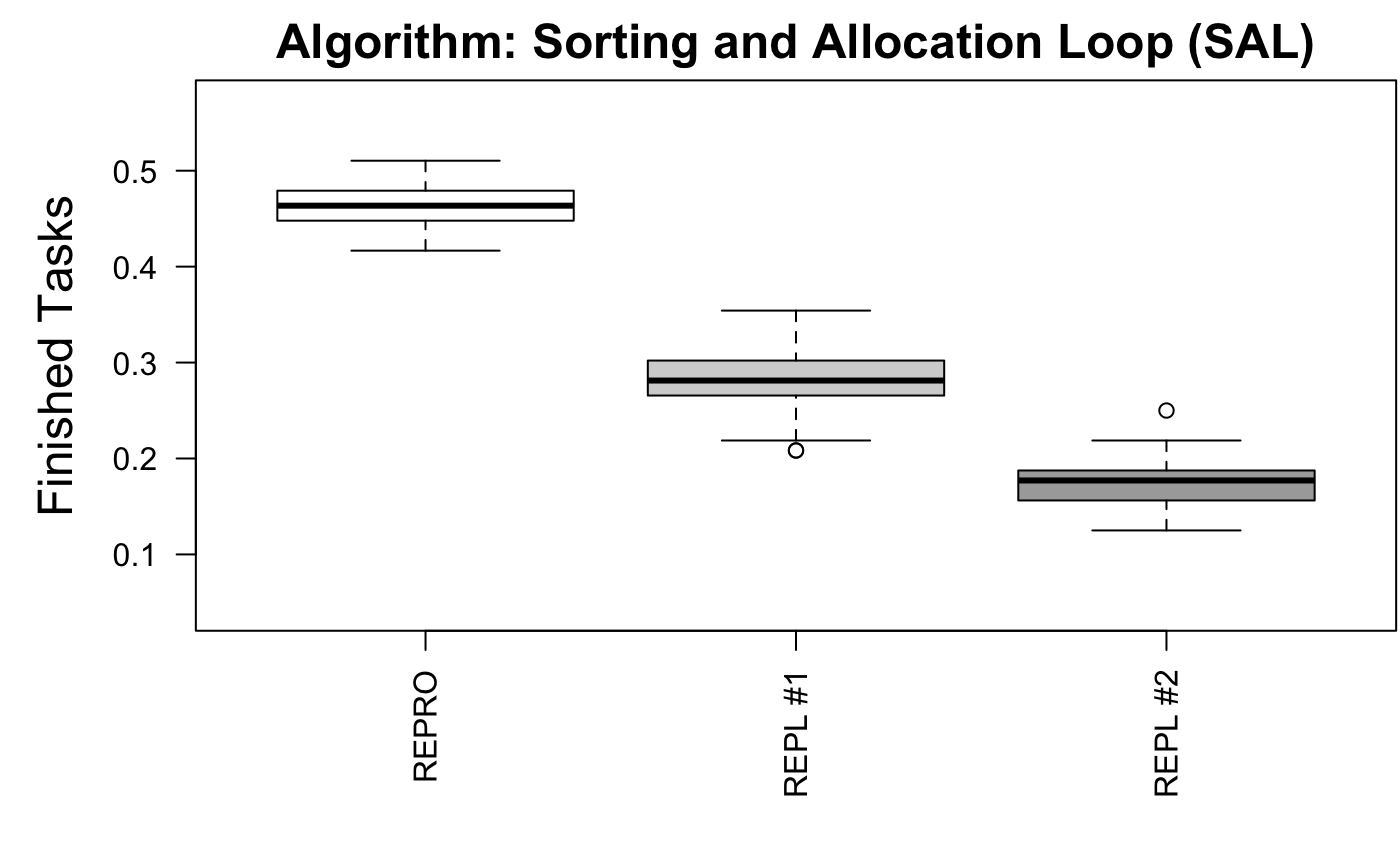
\includegraphics[scale=0.1]{fig/BOX03.png}
}
\caption{Finished tasks to the original algorithm in static scenario (reproduction - REPRO), in the dynamic scenario (first replication - REPL #1) and the extended algorithm in dynamic context (second replication - REPL #2) with the attributes: 96 tasks; 9 UAVs; 300 x 240; 300 ticks and 100 executions}
\label{fig:box01}
\end{figure}

The confirmation of the statistical significance of the difference of such values was obtained by a t-Test, which was employed because the results distribution is close to a normal one, as show in Figure \ref{fig:fig07}. Thus, it is confirmed that the average quality and messages results obtained by the original algorithms and the modified ones are different. The test confirmed the difference with a confidence interval of $0.99$ and $p-val<0.05$. 

\begin{figure}[!htb]
\centering
\subfloat{
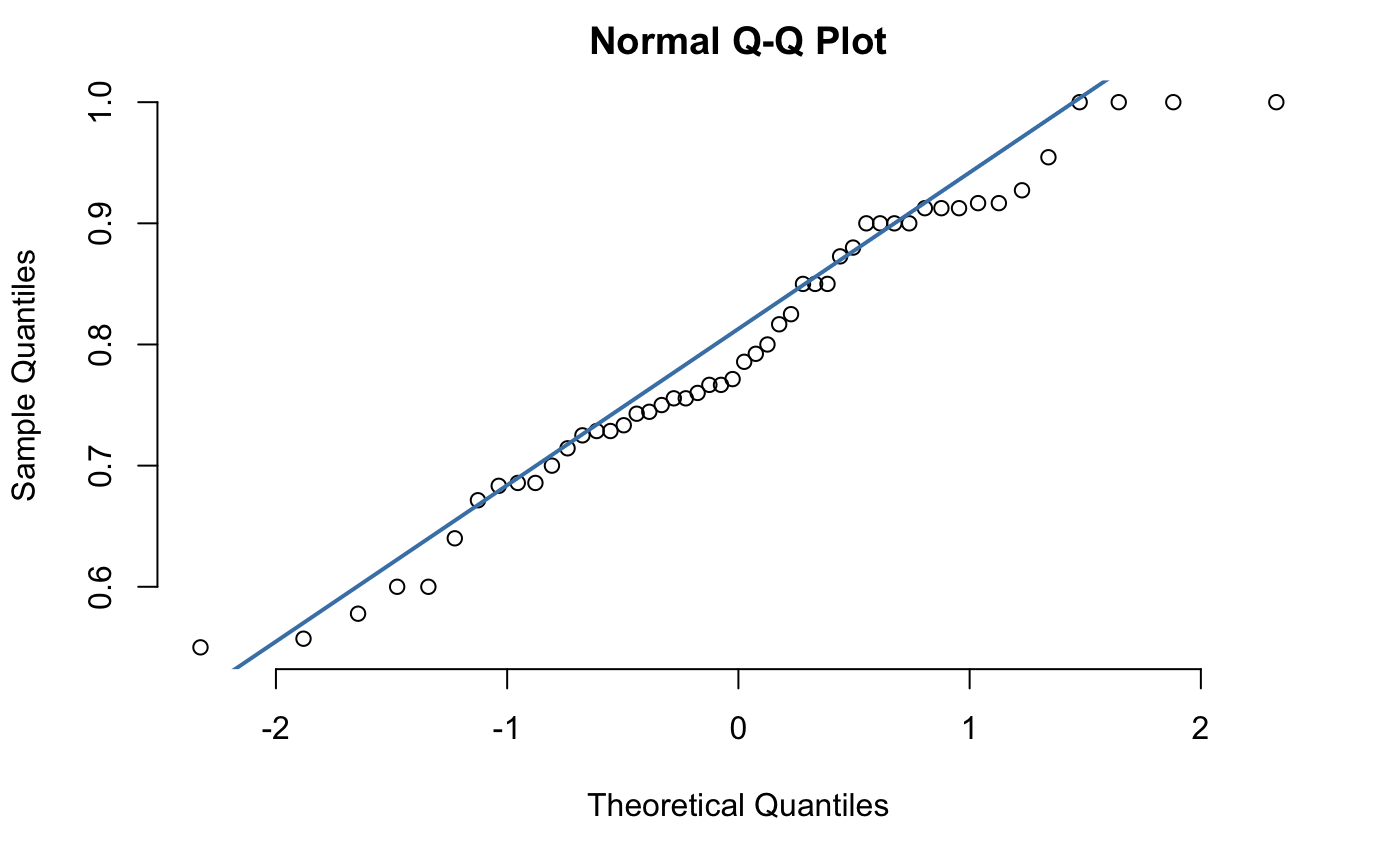
\includegraphics[scale=0.1]{fig/GRAPH09.png}
}
\quad
\subfloat{
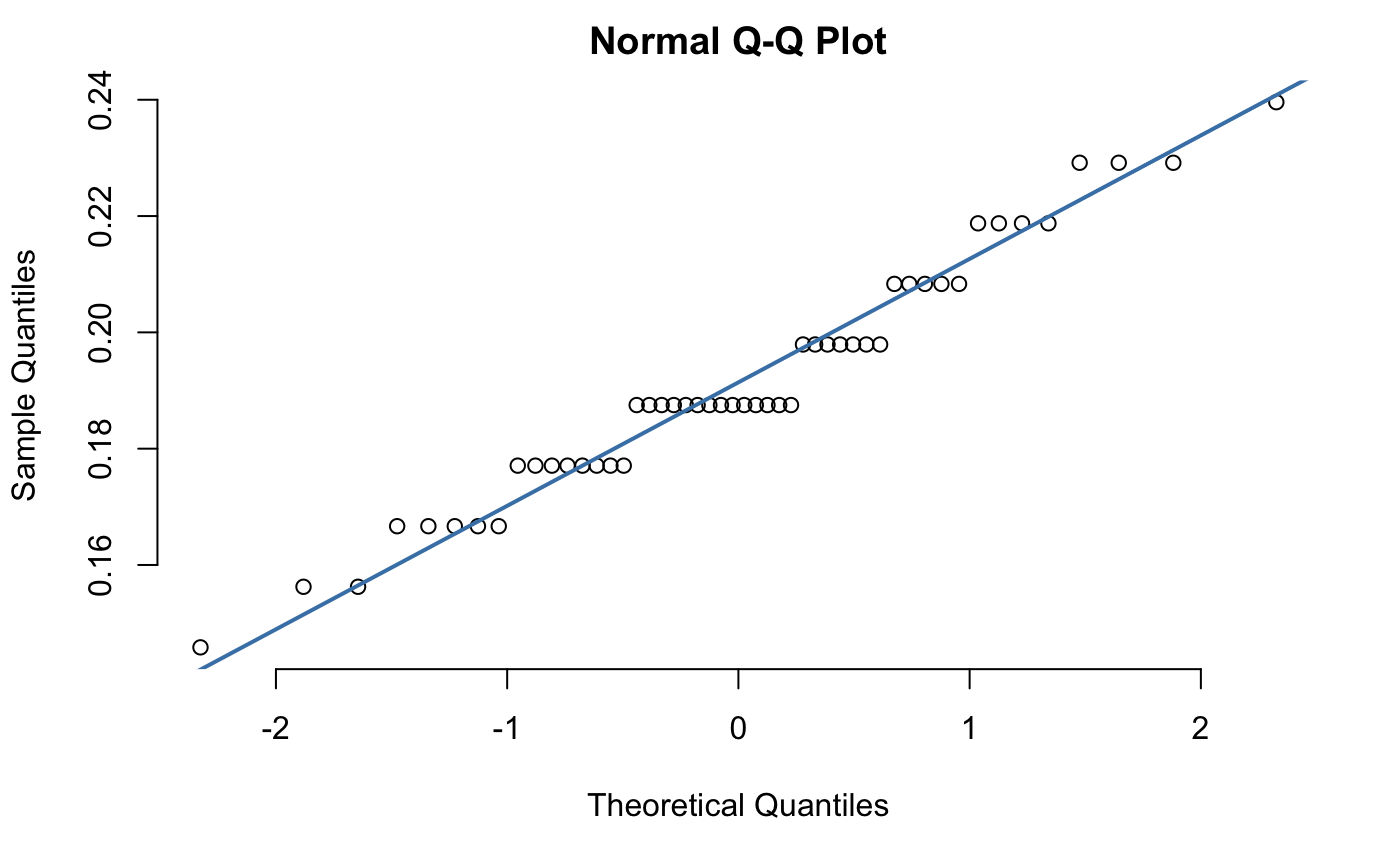
\includegraphics[scale=0.1]{fig/GRAPH10.png}
}
\caption{Distribution of finished tasks (left) and quality (right) results compared with the Normal Graph (Extended SAL algorithm; 96 tasks; 9 UAVs; 300 x 240; 300 ticks; 50 executions)}
\label{fig:fig07}
\end{figure}

For this replication, the $stimulus$ value applied was of $0.6$. It is the same value applied by the original work and the reproduction done in the beginning of the present study (Section \ref{sec:method}). The justification of its use is presented in~\cite{MAS07} and~\cite{ferreira2007swarm}.

As it was done in Section \ref{sec:original}, different values to the \textit{stimulus} attribute were tested. However, when the results obtained with different \textit{stimulus} values were compared, the variation stayed into the standard deviation. To allow a faithful final comparison in this work, the value used by the original work \cite{MAS07} of $0.6$ was also used to this independent variable (Section \ref{sec:discussion}).


\section{Discussion}\label{sec:discussion}
This section aims to identify the main aspects found during the replications done and to analyze all obtained results (see Section \ref{sec:findings}), identifying its implications for practice (see Section \ref{sec:implications}), characterizing the threats to the study validity (see Section \ref{sec:threats}), listing the main existing limitations in this work done and the opportunities to perform further investigations based on this one (see Section \ref{sec:limitations}).

\subsection{Findings}\label{sec:findings}
The replications performed with the original and the extended algorithms, in the dynamic scenario, suggested higher results difference in quality and number of messages sent metrics. These highlighted differences justify choosing these two variables to analyze the algorithms behaviour and the emerging trade-off, in that new dynamic scenario. The messages exchanged represent the token being sent to the next agent in the communication network.

The quality of the sensors related to the tasks guarantees that the agent is the most suitable one to perform it. Figure \ref{fig:fig03} shows a significant quality results decrease with the original algorithms in the dynamic scenario. On the other hand, Figure \ref{fig:fig05} shows that extended algorithms increased this variable results, even with a reduced number of performed tasks, bringing the level to the same original baseline. 

As the first contribution, this work provides evidence that the original algorithms proposed in \cite{MAS07}, and based on Swarm-GAP intelligence, work in dynamic scenarios. However, the results obtained for all variables were not in the same level of what were obtained by the original study in a static context. All dependent variables presented similar values compared with the original study \cite{MAS07}, except the following:

\begin{itemize}
   \item \textbf{Quality}: when the UAVs are disabled (representing a shut down aircraft), the tasks allocated to it are not performed and the quality sum of completed tasks decreased ($\approx 40\%$) as there are fewer agents;
   \item \textbf{Capability}: as the agent capability is calculated using the sensors quality,  and it decreases as explained above, this variable decreases by $\approx 40\%$;
   \item \textbf{Number of finished tasks}: having fewer UAVs to perform the tasks, it is natural that the number of finished tasks decreases. This variation was $\approx 50\%$ in most cases.
   \item \textbf{Elapsed Time}: the time spent to perform the mission was shorter due to the fewer number of UAVs. The remaining UAVs always use the maximum possible available resource to perform the tasks. However, in general such resource exhausted before the total available time. Thereby, the elapsed time reduced in $\approx 15\%$, particularly in LAL and SAL algorithms. The results in those algorithms fall off the standard deviation compared with the original experimental results.
\end{itemize}

Even with the variation above, this solution can be applied in case in which there is no other strategy available to deal with a dynamic scenario. However, there is evidence indicating possibility of algorithms improvement.

In this vein, the second contribution is the improvement proposed to those algorithms to deal better with the proposed dynamic scenario. The extended algorithms presented in Section \ref{sec:changes} was submitted to an independent replication and the results were similar to the original algorithms applied in dynamic scenarios except for following metrics:

\begin{itemize}
   \item \textbf{Quality}: this metric presented a significant result recovery ($\approx +40\%$) showing a level equal to the original study, which was carried out in a static scenario (Section \ref{sec:replication});
   \item \textbf{Number of exchanged messages}: the extended algorithms require more exchanged messages due to the token reset. This characteristic causes an increase of $100\%$ in the number of exchanged messages compared to the original algorithms in the dynamic scenario (Section \ref{sec:replication});
   \item \textbf{Number of finished tasks}: the number of finished tasks reduced up to $50\%$, compared to the original algorithms in the static scenario, due to the required time to resend tokens when something in the dynamic context occurs, i.e., when there is a an UAV removal. With this, there is a fewer number of available UAVs in the experiments.
\end{itemize}

It is possible to notice that, even with a reduced number of finished tasks, the total quality increased due to the tasks reallocation that occurs when a UAV is shut down. This operation always occurs getting the maximum possible quality level based on the available resources, associating the most suitable sensors to the tasks.

Thus, it is possible to increase quality results if the network aspects are not an issue and the communication structure can support the demand required to execute the extended algorithms. Indeed, it was also possible to identify a message traffic 3 times higher than the original one due to the communication need among the agents using the extended algorithms, which provides evidence for the network capability requirement.

In summary, this empirical work provides evidence that there is a trade-off among the quality and the number of exchanged messages when the extended algorithms here proposed are used in dynamic scenarios as described in Section \ref{sec:dynamic_scenario}. The scope of this study is relevant because the dynamic created scenario use assumptions closer to the real world operation scenario, presenting a more realistic (and useful) way to perform tasks allocation.

\subsection{Implications for Practice}\label{sec:implications}
As explained in previous sections, the trade-off that there is among the communication overhead and quality results is an important aspect to be considered when choosing which algorithm to use. The right choice depends on what is the priority. If the allocation needs to be the best according to the sensors available, it is necessary to know that there will be an overhead in communications among the agents. 

In that way, it is necessary to know the network capacity in order to support the messages exchange. Thus, the simulation shows that this aspect is a mandatory requirement to explore the advantages of the modified algorithms. If the communication structure is not good enough or there is no evidence that it supports high volume of messages, it is appropriate reduce the quality result, but to keep a certain level of mission accomplishment.

Based on the replications done, a real scenario described by a set of targets to be photographed can be an example of these algorithms application. Thus, it is necessary to choose if it is more important to have best pictures with more suitable cameras according to the type of targets, or it is necessary to keep the communication structure not overloaded with high quantity of messages (tokens). This example represents a real possible situation where this trade-off needs to be properly analyzed to obtain the best results according to the demand.


\subsection{Threats to Validity}\label{sec:threats}
%Threats to validity
% scenario more dynamic
% other variables change

Basically, the methodology applied in this study was independent replications to collect results to find evidence that the original and extended algorithms are suitable to address the dynamic context. All assessment was done based on these results measured. Thus, for this process, the following threats to validity and corresponding mitigation strategies are presented in the following: 

\begin{itemize}
   \item \textbf{Conclusion validity}: The same code of the original study was used, but during the experiments different results were obtained, although they were in standard deviation compared with those obtained in the previous work, it indicates a variance possibility with changes in the experiment environment. These variations could be increased in case of code changes to implement dynamism. To minimize this threat, a set of tests and analysis were performed using a debug process to minimize undesirable responses due to a bad code manipulation after implementing the dynamism with changes in the number of agents. The results were analyzed to verify correlation and coherent with the new dynamic condition. As the acquired results can varies depending on the hardware configuration, each algorithm was executed a hundred of times to reduce the standard deviation. Furthermore, to comparison means, apparently equals to each other, a t-Test was used to identify these minor differences among the results obtained with the different proposed algorithms, after analyzing their similarity with a normal distribution.
   \item \textbf{Internal validity}: The performance of each algorithm depends on the execution environment. Since the hardware configuration was not the same and the tool version (NetLogo 5.3.1) uses some operating system libraries, there are a slight difference in the results obtained due to these different hardware and software configurations. To minimize this impact, a reproduction of the original study \cite{MAS07} was performed to have a suitable baseline for comparing the replications.
   \item \textbf{Construct validity}: All performed replications used the code obtained with the researcher of the original study, and the documentation lack became an issue in the moment of experiment execution. The modifications done to create the dynamic scenario could generate collateral effects difficult to be identified that could hide some influences and produce non-consistent results. To mitigate this threat, tests and analysis were performed using a debug process to minimize undesirable responses due to a bad code manipulation. Besides that, the same dependent variables were used, as well as units and measurement procedure from the original work, obtaining the results directly from the simulation tool (NetLogo 5.3.1).
   \item \textbf{External validity}: The extended algorithms here proposed were applied in a dynamic scenario where only the number of agents changes. Although the algorithms presented a good performance in this scenario, other elements can change in a real world. The number of tasks, type of tasks, status of the onboard sensors and other context issues that can occur in a real military operation. However, it was possible to approximate the original study, made in a static context, to something closer to the real world. This improvement allows an approach using Swarm-GAP intelligence in a context with a certain level of dynamism.
\end{itemize}



\subsection{Limitations and Future Work}\label{sec:limitations}
The extended algorithms proposed in this work caused more than 100\% of increase in the number of exchanged messages. This result suggests an existence of network requirements to support the necessary communication. Based on this, it is necessary to detail these requirements to guarantee the possibility of plan which algorithm will be chosen according to the available network resources. Some simulations with the proposed algorithms provide evidence about the relations among communication constraints and the quality level desired in the mission accomplishment.

The configuration used by the simulation as a communication structure was a ring network. It would be necessary to assess the impact of using the new proposed algorithms applied on another type of network structure, e.g., in a fully connected network. Maybe another architecture can be more compatible and support a higher demand of message exchanging.

Another opportunity to improvement is to model and to implement a scenario with more dynamic elements. In this work, only the number of agents were changed, but in a real military operation scenario it could have mission/tasks or agents capabilities changing during runtime. With this new context, other impact may be observed and may required variations of the proposed algorithms or even the original Swarm GAP strategy.

These are situations opened as prospective directions for future investigations. Empirical experiments have to be performed to evaluate correlations among the network structure and the algorithm applied to solve the task allocation problem with a scenario plenty of dynamic elements and adopting Swarm-GAP strategy and its variations.


\section{Related Work} \label{sec:related_works}
The works presented by \textit{Alighanbari and How}\cite{alighanbari2005decentralized} and \textit{Schwarzrock et al.}\cite{MAS07} provide the task assignment for a fleet of UAVs, having a decentralized structure with no central command, and running only in static context. The algorithms presented by them were not tested in scenarios were changes can occur during the execution, e.g., the number of agents or tasks changes while the mission is being performed. However, both works mentioned a necessity of reassign tasks in case of any scenario parameter change, leaving an idea to future work. This idea was used in our study to suggest a token reset by the algorithm.

Our work presents a proposal inspired in what was shown by \textit{Schwarzrock et al.}\cite{MAS07} and topics related with tasks allocation and Multi-Agent Systems(MAS) presented by other authors \cite{MAS01, MAS02, MAS03, MAS04, MAS05, MAS06}, extending applied concepts to dynamic context. Although there are centralized solutions to this problem, such as what was presented by \textit{Jose and Pratihar}\cite{jose2016task}, that uses genetic algorithm to assign tasks to a set of robots in a inspection system, this kind of solution is not suitable to the present work because in our scenario there is no guarantee of communication among all elements.

Multiobjective Optimization Problems (MOP) are represented by a vector of decisions satisfying some constraints and aim to optimize a vector of functions that represents an objective. The number of constraints must be less or equals to the number of elements in decision vector, otherwise it is created a problem called as over-constrained. In this scenario, as shown by Coello et al.\cite{MOEA01},  multiobjective evolutionary algorithms (MOEA) appear as a powerful tool to analyze all objectives and their constraints, maximizing global results. This optimization is done with rounds of data analysis trying to converge to the better response. Zitzler et al.\cite{07} compared some approaches to solve MOP and it is possible to identify a common characteristic in the communication protocol that defines a way to redistribute the functions aiming to optimize results. We used this strategy applying more than one communication round in the extended algorithms here proposed.

Ferreira et al. \cite{ferreira2007swarm} provided evidence that the $stimulus$ value of $0.6$ generates best results when applied to calculate the capability of task execution by the agent. However, that analysis was done based on a static scenario. Our work identified a slight difference of $\simeq 3\%$ in results when applied different $stimulus$ in dynamic context. For a fair comparison with the original study \cite{MAS07} and considering the small difference in results, we adopted the value of $0.6$ for this variable.

Many works \cite{ferreira2007swarm,scerri2005allocatingLADCOP, ferreira2010robocup,ikemoto2010adaptive} deal with the allocation task problem. In those studies, the organization and tasks ordering are done by a central command unit. However, this strategy generates a huge amount of messages to transmit the tasks and it can cause a network overhead. To deal with this, the strategy adopted by \textit{Schwarzrock et al.}\cite{MAS07} was the Swarm-GAP, so that it is easier to add agents in the structure or even to treat sensors onboard issues. Our work follows the same strategy based on the requirement of decentralized structure of decision using swarm intelligence.

\section{Conclusion} \label{sec:conclusions}
Since the original work \cite{MAS07} is classified as a reproducible research\cite{exp02} and confirmed by the reproduction displayed in Section \ref{sec:background}, we performed two independent replications, using NetLogo 5.3.1 environment, to collect results and obtain evidences about limitations and improvements opportunities proposed by the present study.

With an approaching closer to real world, we defined a dynamic context in substitution of the original static one used in \cite{MAS07}, and performed a first replication to validate that the original algorithms proposed by \textit{Schwarzrock et al.} are fully functional in this new dynamic scenario. This experiment showed an improvement opportunity due to a decrease in some dependent variables, e.g., capability and quality. 

Proceeding an action research and based on results obtained by the original work, we proposed extended algorithms to better address the new dynamic scenario created. The second replication, assessed these extended algorithms and permitted to identify and discuss emerging trade-offs. The variables quality and exchanged messages were the focus of these analysis due to the variance presented by the extended algorithms in these variables compared with the original ones.

The proposal here presented has, as the main idea, all tasks releasing after the team loose an agent, and the token resetting to permit a new turn of allocation execution steps. Thus, the tasks not completed can be reallocated always looking for the quality maximization based on the relation among the task distance and the sensor suitability to its realization. There are evidences that this new procedure execution requires more communication since the number of exchanged messages increased more than 100\%.

The main discussion is the collateral effect caused to obtain a quality increasing. This effect is an increase in the exchanged messages that suggested some idea of network requirement level to apply the algorithms proposed. However, this measure of network level requirements is left as suggestion of future work. Furthermore, the communication structure used, initially a ring network, can impact in results and different typologies can be tested in the future.


\section*{References}
\bibliographystyle{elsarticle-num}
\bibliography{references}

\end{document}